\documentclass[11pt]{amsart}
\usepackage{geometry}                % See geometry.pdf to learn the layout options. There are lots.
\geometry{letterpaper}                   % ... or a4paper or a5paper or ... 
%\geometry{landscape}                % Activate for for rotated page geometry
%\usepackage[parfill]{parskip}    % Activate to begin paragraphs with an empty line rather than an indent
\usepackage{subfig}
\usepackage{graphicx}
\usepackage{caption}
% \usepackage{subcaption}
\usepackage{amssymb}
\usepackage{epstopdf}
\usepackage{amsmath, amsthm, amssymb}
\usepackage[ansinew]{inputenc}
\usepackage{bbm}
\usepackage{cancel}
\usepackage{mathdots}
\usepackage{natbib}

\usepackage{color}   %May be necessary if you want to color links
\usepackage{hyperref}
\hypersetup{
    colorlinks=true, %set true if you want colored links
    linktoc=all,     %set to all if you want both sections and subsections linked
    linkcolor=blue,  %choose some color if you want links to stand out
}

\DeclareGraphicsRule{.tif}{png}{.png}{`convert #1 `dirname #1`/`basename #1 .tif`.png}
% \setlength\parindent{0pt}

\usepackage{algorithm}
\usepackage[noend]{algpseudocode}

\let\biconditional\leftrightarrow
\newcommand{\indep}{\rotatebox[origin=c]{90}{$\models$}}
\newcommand{\p}{\text{p}}

\DeclareMathOperator*{\argmax}{\arg\!\max}

\makeatletter
\def\BState{\State\hskip-\ALG@thistlm}
\makeatother

\title{Last Chance Stats}
\author{Joseph Boyd}
%\date{}                                           % Activate to display a given date or no date

\begin{document}
\maketitle

\tableofcontents

\pagebreak

\section{Warm Up}

This section presents an assortment of mathematical problems, each embodying an idea that is useful or instructive to the material that follows.

\subsection{Proof of Pythagorean Theorem}

Consider a square with sides of length $c$ rotated inside a larger square, such that the four corners of the smaller square meet a distinct edge of the larger at a point $a$ units along that edge. The sides of the larger square are therefore of length $a + b$ for some $a, b > 0$. The area of the four resulting right-angled triangles that fill the empty space are $\frac{1}{2}ab$ apiece. Thus, we have it that, $$(a + b)^2 = c^2 + 4 \cdot \frac{1}{2}ab,$$ expanding to, $$a^2 + 2ab + b^2 = c^2 + 2ab,$$ and finally, $$a^2 + b^2 = c^2.$$

\subsection{Irrationality of $\sqrt{2}$}

Suppose $\sqrt{2}$ is rational. Then there exist $a, b \in \mathbb{Z}$, with $a > b$ and $gcd(a, b) = 1$\footnote{That is, $\frac{a}{b}$ is an irreducible fraction. This can be obtained by cancelling out the common factors. Every integer has a unique prime factorisation due to the fundamental theorem of arithmetic.} such that, $$\frac{a}{b} = \sqrt{2}.$$

Consequently, $$\frac{a^2}{b^2} = 2.$$ This implies that $a^2$ is even, and therefore that $a$ is even. That is, $$a = 2k,$$ for some $k \in \mathbb{Z}$. So, by substitution, $$\frac{4k^2}{b^2} = 2.$$ Rearranging, $$b^2 = 2k^2.$$ However, this now implies that $b^2$ is even, hence $b$ also, implying a common factor between $a$ and $b$, though by assumption they have no common factors, and clearly we can repeat the argument ad infinitum. This contradiction proves $\sqrt{2}$ is irrational\footnote{This is an example of a proof by contradiction.}.

\subsection{Euclid's Proof of the Infinitude of Primes}

Take any finite set of primes, $p_1, p_2, \dots, p_n$. Then, the number, $q = p_1 \times p_2 \times \cdots \times p_n + 1$, is either prime or not prime. If it is prime, we have generated a new prime not in our set. If it is not, it has a prime factor not in our set, as $q \equiv 1 \ (\text{mod}\ p_i)$ for $i = 1, 2, \dots, n$. Using this method we can always generate a new prime\footnote{This is an example of a constructive proof.}.  It follows that there are infinitely many primes.

\subsection{The Potato Paradox}

A potato that is $99\%$ water weighs 100g. It is dried until it is only $98\%$ water. It now weighs only 50g. How can this be?

The mistake people typically make is to assume there has been a $1\%$ reduction in the volume of water, rather than a change to the water/non-water ratio. In fact, the ratio of water to non-water content has changed from $1:99$ to $2:98$ or $1:49$. Since the non-water content of the potato has not changed, the water must have lost $50\%$ of its volume, and so the potato now weighs half as much!

\subsection{The Monty Hall Problem}

This famous paradox, named after an American game show host, has the following problem statement:

\emph{A game show presents you with the choice of selecting one of three doors. Two of the doors contain a goat (undesirable), whilst the third contains a car. Upon your choice, the game show host, who knows the contents of each of the doors, opens one of the two remaining doors to reveal a goat. He then gives you the option of either sticking with your initial choice, or switching to the one remaining door. Is it advantageous to switch doors?}

The answer is that it \emph{is} advantageous, increasing your winning chances from $1/3$ to $2/3$. The essential realisation is that the host (Monty Hall) has knowledge of the door contents and will always reveal a goat, whether you have chosen the car or not.

The solution can be understood as a decision theory problem. We designate two strategies: changing and not changing doors. In either case, there is a $2/3$ chance of initially having a goat. Because the other goat is eliminated independently by the host, changing wins whenever a goat was initially chosen, that is, with probability $2/3$. Not changing wins only if the car was initially chosen, that is, with probability $1/3$. Therefore changing will double your winning chances!

Another (admittedly more complicated) way to solve the problem is using Bayes' theorem. Here we designate $C_1, C_2$, and $C_3$ as the events the car is behind doors 1, 2, and 3 respectively; $X_1$ the event the player chooses door 1; and $H_3$ the event the host opens door 3. Note the numbering of the doors does not matter. For example, `door 2' simply refers to `the other door'. First, $\text{Pr}(H_3|C_1,X_1) = 1/2$, $\text{Pr}(H_3|C_2,X_1) = 1$, and $\text{Pr}(H_3|C_3,X_1) = 0$, reflecting the knowledge that the host always opens a goat door (never the car). Then,

\begin{align}
\text{Pr}(C_2|X_1,H_3) &= \frac{\text{Pr}(H_3|C_2,X_1)\text{Pr}(C_2|X_1)}{\text{Pr}(H_3|X_1)} \notag \\
&= \frac{\text{Pr}(H_3|C_2,X_1)\text{Pr}(C_2|X_1)}{\text{Pr}(H_3|C_1,X_1)\text{Pr}(C_1|X_1) + \text{Pr}(H_3|C_2,X_1)\text{Pr}(C_2|X_1) + \text{Pr}(H_3|C_3,X_1)\text{Pr}(C_3|X_1)} \notag \\
&= \frac{1 \cdot 1/3}{1/2 \cdot 1/3 + 1 \cdot 1/3 + 0 \cdot 1/3} \notag \\
&= \frac{2}{3}, \notag
\end{align}

so the winning odds for changing doors is $2/3$, hence not changing only $1/3$.

\subsection{Finding Hamlet in the Digits of $\pi$}

It is supposed, though not known for certain, that $\pi$ is a normal number. This means that in the infinitely many decimal digits of $\pi$, every sequence of $n$ digits appears as often as every other length $n$ sequence. So, 123 occurs as often as 321 or 666, but more often than 123456789, because it is a shorter sequence. In this way, the behaviour of the digits of $\pi$ is indistinguishable to what would arise from a uniform random distribution. Of course, the digits of $\pi$ are not random, as many formulas exist for generating them. The same rules of normalness apply if $\pi$ is converted to a different base, for example, binary code--the number system of computer arithmetic. The number $\pi$ in binary is,

\begin{align}
\pi &= 3.14... \notag \\
&= 1\cdot2^1 + 1\cdot2^0 + 0\cdot2^{-1} + 0\cdot2^{-2} + 1\cdot2^{-3} + 0\cdot2^{-4} + 0\cdot2^{-5} + 1\cdot2^{-6} + \cdots \notag \\
&= 11.001001... \notag
\end{align}

Note that to express $\pi$ in binary rather than decimal notation requires more digits, because it takes $\log_2(10) \approx 3.3$ binary digits (bits) to express each power of ten. Nevertheless, the same properties about the normalness of $\pi$ hold in its binary form--$000$ is just as likely as $111$, and so on.

Now, to find Hamlet, we would need to start with a common base. Hamlet is written in Latin characters. One way to convert Latin characters to numbers is to use a character encoding standard, such as ASCII (American Standard Code for Information Interchange). People use ASCII indirectly every day--it is how our data comes to be represented by computers and communication systems. ASCII gives a representation of each character in 8 binary digits. For example, in ASCII,

$$\text{``pie''} = 01110000 \ 01101001 \ 01100101.$$

So, Hamlet, like any text, has an ASCII, and therefore binary representation. Without specifying exactly what it is we can determine its length. There are 186,391 characters in the 31,842 word Hamlet, including spaces and indentation. At 8 bits per character, this is 1,491,128 bits.

To develop a formula, we first consider a simpler problem: what is the expected number of digits we should pass over in a random binary sequence before we encounter a specific binary sub-sequence, say, 11? If we consider a binary tree covering all the possibilities, and let the expected length to find 11 be denoted by $\mathbb{E}_{11}$, then we may first see 0 with probability $\frac{1}{2}$, in which case we are back to where we started. That is, the first digit is a failure, because it is not the one we are looking for. The expected length from there is therefore $1 + \mathbb{E}_{11}$. We might alternatively see 1 in the first digit--a match--also with probability $\frac{1}{2}$. In this case, the next digit is 0 with probability $\frac{1}{2}$, which would mean a failure on the second digit, and again, we return to the starting point, with expected length now $2 + \mathbb{E}_{11}$. Otherwise, we could get a 1 in the second digit, and we have found the match straight away. In this case, the expected length is simply 2. Therefore we may write,

$$\mathbb{E}_{11} = \frac{1}{2}\times(1 + \mathbb{E}_{11}) + \frac{1}{4}\times (2 + \mathbb{E}_{11}) + \frac{1}{4}\times 2,$$

which we may solve to find $\mathbb{E}_{11} = 6$. That is, we expect to pass over $6$ binary digits (on average) before we see the particular sequence, 11. We see that in general, it is possible to fail on each of the $n$ digits in the sequence. Thus, we have the following expression for the general $n$-bit sequence,

$$\frac{1}{2^n}\mathbb{E}_{\{0, 1\}^n} = 1\times\frac{1}{2^1} + 2\times\frac{1}{2^2} + 3\times\frac{1}{2^3} + \cdots + 2n\times\frac{1}{2^{n}}.$$

If we denote this sum $S$ then clearly,

\begin{align}
S - \frac{1}{2}S &= 1\times\frac{1}{2^1} + 1\times\frac{1}{2^2} + 1\times\frac{1}{2^3} + \cdots + 1\times\frac{1}{2^{n}} = 1 - \frac{1}{2^{n}} \notag \\
&\implies S = 2 - \frac{1}{2^{n-1}}, \notag
\end{align}

hence, $\mathbb{E}_{\{0, 1\}^n} = 2^{n+1} - 2$. Applying this formula, we can expect to find Hamlet somewhere within the first $2^{1,491,129} - 2 \approx 3.6\times10^{448,874}$ digits of $\pi$.

\section{Differential Calculus}

This section presents the fundamental results of differential calculus: first the formal definition of a limit, then that of a derivative. In particular, we note the relationship between the binomial theorem and the differentiation of polynomials. The section culminates with a proof of the mean value theorem.

\subsection{Binomial Theorem}

The binomial theorem expresses a formula for expanding powers of a binomial\footnote{A binomial is the sum of two \emph{monomials}, that is, a polynomial with a single term.}. For example, $(x + y)^3 = x^3 + 3x^2y + 3xy^2 + y^3$. In general, the binomial expansion is,

$$(x + y)^n = \sum_{k = 0}^{n}{{n}\choose{k}}x^ky^{n-k},$$

where, $${{n}\choose{k}} = \frac{n!}{k!(n-k)!},$$ is known as the binomial coefficient. Note the binomial coefficient is symmetric, that is, ${{n}\choose{k}} = {{n}\choose{n-k}}$. This symmetry may be seen in Pascal's triangle,

\begin{center}
\begin{tabular}{ccccccccccccc}
&&&&&&1&&&&&& \\
&&&&&1&&1&&&&& \\
&&&&1&&2&&1&&&& \\
&&&1&&3&&3&&1&&& \\
&&1&&4&&6&&4&&1&& \\
&1&&5&&10&&10&&5&&1& \\
1&&6&&15&&20&&15&&6&&1 \\
\end{tabular}
\end{center}

where each number is the binomial coefficient with $n$ the row number and $k$ the column. Pascal's triangle is named after French mathematician Blaise Pascal (1623-1662). Note that each number is the sum of the two numbers diagonally above. In terms of binomial expansion, this is equivalent to collecting like terms after expanding. To illustrate, consider the coefficients for the quadratic expansion, $x^2 + 2xy + y^2$,

\begin{center}
\begin{tabular}{ccccc}
1&&2&&1\\
\end{tabular}
\end{center}

Multiplying again by the binomial, $(x + y)$, gives the coefficients,

\begin{center}
\begin{tabular}{cccccccccccccccc}
1&&1&&2&&2&&1&&1 \\
\end{tabular}
\end{center}

which corresponds to $x^3 + x^2y + 2x^2y + 2xy^2 + xy^2 + y^3$, and clearly each of the interior pairs are like terms, so these are summed to arrive at,

\begin{center}
\begin{tabular}{cccccccccc}
1&&3&&3&&1 \\
\end{tabular}
\end{center}

In general, this relation is reflected in Pascal's rule,

$${{n}\choose{k}} = {{n-1}\choose{k-1}} + {{n-1}\choose{k}},$$
		
for $1 \leq k \leq n$. Isaac Newton (1642-1727) extended the notion of binomial expansion to real powers in 1665. This was an important stepping-stone towards the definition of a derivative, as we will see.

\subsection{($\epsilon$-$\delta$) Definition of a Limit}

The standard formal ($\epsilon$-$\delta$) definition of a limit is due to German mathematician, Karl Weierstrass (1815-1897). We say that, $$\lim_{x \to a} f(x) = L,$$

if for any value, $\epsilon > 0$, specifically where $\epsilon$ is arbitrarily small, we can find a value $\delta > 0$ such that,

$$0 < |x - a| < \delta \implies |f(x) - L| < \epsilon.$$

This somewhat off-putting notation captures the notion of a function approaching a limiting value continuously. It states that however close (within an infinitesimal $\epsilon$ units) we wish to get to the limiting value, $L$, we can always find a correspondingly tiny interval of radius $\delta$ around the limiting point $a$ such that the function is closer. Note that this accounts also for the case where $f(x)$ is undefined at $x = a$.

An example is always useful for such subtle ideas. Therefore, let $f(x) = 2x^2 + 2$. Then clearly, $\lim_{x \to 0} f(x) = 2$. To satisfy the inequality, $|2x^2 + 2 - 4| < \epsilon$, we can select $\delta = \sqrt{\epsilon/2 + 1}$. Clearly this is always possible, no matter how small we take $\epsilon$ to be, and so the limit exists.

A function is said to be \emph{continuous} at a point $a$ if the limit $L$ exists, and $f(a) = L$, which is not always the case. Suppose $g(x) = 1$ for $x <0$ and $g(x) = 2$ for $x \geq 0$. Such a function makes an instantaneous jump at $x = 0$ to a value distinct from the limit to which it was approaching, and is therefore \emph{discontinuous} and does not satisfy the $\epsilon$-$\delta$ condition. Alternatively, the limit may exist, but the function may not be defined at the limiting point, thus also a discontinuity. A function is continuous if it is continuous at all points in its domain. A function that is \emph{differentiable} at a point, $a$, implies continuity at $a$, but not vice-versa. For example, the absolute value function, $f(x) = \text{abs}(x)$ is continuous but not differentiable. Differentiability of a function at a point roughly means it is possible to measure the \emph{trajectory} of the function at that point, so that it is possible to draw a tangent line at that point.

\subsection{Differentiating From First Principles}

The gradient of a linear function, $y = f(x)$, over an interval, $[x, \Delta x]$, is defined as $\Delta y / \Delta x$, that is, `rise over run'. The derivative of a function is simply the gradient taken at a point. Formally, we define a derivative as,

$$\frac{\mathop{d}}{\mathop{dx}} f(x) = \lim_{\Delta x \to 0} \frac{f(x  + \Delta x) - f(x)}{\Delta x},$$

and it is clear this is just `rise over run', albeit taken on an infinitesimal interval. It represents the gradient of a line tangent to the curve at $x$. To see how we can differentiate a polynomial, consider the general $n$th degree polynomial\footnote{Note that the powers of a polynomial are non-negative integers by definition.}, $f(x) = a_nx^n + a_{n-1}x^{n-1} + \cdots + a_1x + a_0$. Then, from the definition,

\begin{align}
\frac{\mathop{d}}{\mathop{dx}} f(x) &= \lim_{\Delta x \to 0} a_n\frac{(x + \Delta x)^n - x^n}{\Delta x} + \cdots + a_1\frac{(x + \Delta x) - x}{\Delta x} + a_0\frac{1 - 1}{\Delta x}\notag \\
&= \lim_{\Delta x \to 0} a_n\frac{{{n}\choose{0}}x^n + {{n}\choose{1}}x^{n-1}\Delta x + \cdots + {{n}\choose{n}}(\Delta x)^n - x^n}{\Delta x} + \cdots + a_1\frac{\Delta x}{\Delta x} + a_0\frac{0}{\Delta x} \notag \\
&= na_nx^{n-1} + (n-1)a_{n-1}x^{n-2} + \cdots + a_1, \notag
\end{align}

and it is clear that only the second term of each expansion survives cancelation, or annihilation by the infinitesimal $\Delta x$. From this we can infer that $\frac{\mathop{d}}{\mathop{dx}} a_kx^k = ka_kx^{k-1}$, the rule that every student of calculus is familiar with, though usually does not realise it to be a consequence of the binomial theorem! It is only when one tries to `plug and play' from first principles that these connections become apparent. As noted before, Newton extended the definition of the binomial theorem to real-valued powers.

\subsection{Chain Rule}

The chain rule for differentiation describes how to differentiate function compositions, $f \cdot u \triangleq f(u(x))$. Assuming $u(x)$ is differentiable at $a$, and $f(u)$ is differentiable at $u(a)$, the derivative,

\begin{align}
(f \cdot u)'(a) &= \lim_{x \to a}\frac{f(u(x)) - f(u(a))}{x - a} \notag \\
&= \lim_{x \to a}\frac{f(u(x)) - f(u(a))}{u(x) - u(a)} \cdot \frac{u(x) - u(a)}{x - a} \notag \\
&= f'(u(a))u'(a). \notag
\end{align}

An extension to this expression is needed for a rigorous proof, as a function may oscillate as it tends towards a limit, and $u(x)$ may equal $u(a)$ infinitely many times, resulting in a inexhaustible number of undefined points as $x \to a$, but we will leave it as a sketch.

In general, the chain rule may be applied repeatedly for any number of nested functions,

$$\frac{\mathop{d}}{\mathop{dx}} f_n(f_{n-1}(\cdots (f_1(x)))) = \frac{\mathop{df_n}}{\mathop{df_{n-1}}}\cdot \frac{\mathop{df_{n-1}}}{\mathop{df_{n-2}}} \cdot \cdots \cdot \frac{\mathop{df_2}}{\mathop{df_1}}\cdot \frac{\mathop{df_1}}{\mathop{dx}}.$$

The corresponding technique for anti-differentiation is \emph{integration by substitution}.

\subsection{Product Rule}

The product rule for differentiation allows us to differentiate products of functions of $x$. Suppose $f(x) = u(x)v(x)$. Then, from first principles,

\begin{align}
f'(x) &= \lim_{\Delta x \to 0} \frac{f(x + \Delta x) - f(x)}{\Delta x} \notag \\
&= \lim_{\Delta x \to 0} \frac{u(x + \Delta x)v(x + \Delta x) - u(x)v(x)}{\Delta x} \notag \\
&= \lim_{\Delta x \to 0} \frac{u(x + \Delta x)v(x + \Delta x) - u(x)v(x + \Delta x) + u(x)v(x + \Delta x) - u(x)v(x)}{\Delta x} \notag \\
&= \lim_{\Delta x \to 0} \frac{u(x + \Delta x) - u(x)}{\Delta x}\cdot v(x + \Delta x) + \frac{v(x + \Delta x) - v(x)}{\Delta x}\cdot u(x)\notag \\
&= u'(x)v(x) + v'(x)u(x). \notag
\end{align}

The quotient rule can be derived by applying both the product rule and the chain rule. For $f(x) = u(x) / v(x)$, write, $f(x) = u(x)v(x)^{-1}$. Then, 

\begin{align}
\frac{\mathop{d}}{\mathop{dx}}f(x) &= u'(x)v(x)^{-1} - u(x)v'(x)v(x)^{-2} \notag \\
&= \frac{u'(x)v(x) - u(x)v'(x)}{v(x)^2}. \notag
\end{align}

The corresponding technique for anti-differentiation is \emph{integration by parts}.

\subsection{Rolle's Theorem}

Rolle's theorem by Michel Rolle (1652-1719) asserts that for a differentiable function, $f(x)$, if $f(a) = f(b)$ for some $a$ and $b$, then there must be a stationary point on the interval $[a, b]$, unless $f = c$ for some constant, $c$. Plainly speaking, it says that if a curve returns to its starting point at the end of an interval, there must be at least one turning point somewhere in that interval. To prove this, first consider that there must be at least one extreme point $c$ on the interval $[a, b]$, be it maximum or minimum. For brevity, we assume that $c$ is a maximum. So, for all points after the interior point, $c$, $c + h$, such that $h > 0$, the function is upper-bound by $f(c)$. That is,

$$\frac{f(c + h) - f(c)}{h} \leq 0.$$

Taking the limit gives,

$$f'(c) = \lim_{h \to 0^+} \frac{f(c + h) - f(c)}{h} \leq 0.$$

Likewise, for $h < 0$ we have,

$$f'(c) = \lim_{h \to 0^-} \frac{f(c + h) - f(c)}{h} \geq 0,$$

from which it follows that the derivative of the function, $f'(x)$, is 0 at $c$.

\subsection{Mean Value Theorem}

The mean value theorem states that for a differentiable function defined on an interval $[a, b]$, at least one point on the curve must have gradient equal to that of the chord connecting the endpoints, $(a, f(a))$ and $(b, f(b))$. It is an intuitive result, as any curve which succeeds in climbing (or descending) from $f(a)$ to $f(b)$, must match the rise over run of that slope at least at one point, otherwise it will not complete the ascent.

First, define $g(x) = f(x) - rx$. This must be differentiable on $[a, b]$ since $f(x)$ is by construction. We choose $r$ such that $g(x)$ satisfies Rolle's theorem, that is, $g(a) = g(b)$, hence $f(a) - ra = f(b) - rb$, and $r = (f(a) - f(b))/(a - b)$, that is, the slope of the chord connecting the endpoints. Because of Rolle's theorem, for some $c \in [a, b], g'(c) = 0,$ hence $f'(c) = r$, and the proof is complete.

\section{Linear Algebra}

A set of $M$ equations in $N$ variables can be referred to as a \emph{system of linear equations}. Each variable may feature in one or more of the $M$ equations. We are typically interested in finding a \emph{simultaneous solution}, that is, values for each of the variables satisfying all the equations at the same time. If $M < N$ (more variables than equations), the system is \emph{underdetermined}. In this case, there will not be enough information to identify a unique solution, and the solution will be expressed in terms of at least one of the variables, giving an infinite family of solutions. If any equations are mutually contradictory\footnote{For example, the equations $x + y + z = 1$ and $x + y + z = 2$ have no simultaneous solution.}, however, the system will have no solution. If $M > N$, the system is \emph{overdetermined}. Unless the excess equations are in fact linear combinations of others, the solution will necessarily have mutually contradictory equations\footnote{If the left-hand sides of some group of $N$ of the $M$ equations are linearly independent, they form a basis in $\mathbb{R}^N$. Therefore, the left-hand side of any excess equation is some linear combination of this group of $N$. The right-hand side of the excess equation must be equal to the corresponding linear combination of the $N$ right-hand sides, or else it is in contradiction, and the overall system has no solution.}. A system of linear equations may alternatively be written as a matrix equation,

$$\mathbf{A}\mathbf{x} = \mathbf{b},$$

where $\mathbf{A}$ is the matrix of coefficients, $\mathbf{x}$ is vector form of the simultaneous solution, and $\mathbf{b}$ is the vector of constants. The solution, $\mathbf{x}$, may therefore be found by inverting $\mathbf{A}$. A square matrix $\mathbf{A} \in \mathbb{R}^{N\times N}$ is invertible or non-singular if there is a matrix $\mathbf{A}^{-1} \in \mathbb{R}^{N\times N}$ such that $\mathbf{A}\mathbf{A}^{-1} = \mathbf{A}^{-1}\mathbf{A} = \mathbf{I}$. Non-square matrices can have at most distinct left or right inverses. There are many matrix properties necessary and sufficient for invertibility. In particular, the rows and columns of $\mathbf{A}$ are linearly independent and span\footnote{The span of a set of vectors is intuitively its expressiveness as a basis. $N$ linearly independent vectors form a basis for the vector space $\mathbb{R}^{N}$. On the other hand, if there are linear dependencies in the system, the span will be of lower dimension.} the vector space $\mathbb{R}^{N}$. This is equivalent to having full rank, which is in turn equivalent to having zero nullity\footnote{The rank of a matrix, $\mathbf{A}$ is the dimensionality of the vector space spanned with its columns as a basis. This is always equivalent to the span of its rows (row rank of $\mathbf{A}$). The nullity of a matrix is the dimensionality of its null space, that is, the set of all vectors solving $\mathbf{A}\mathbf{x} = \mathbf{0}$.}. These properties are connected in the rank-nullity theorem\footnote{The rank-nullity theorem states that for $N \times N$ matrix, $\mathbf{A}$, its rank and nullity sum to its number of columns, formally, $\text{rank}(\mathbf{A}) + \text{null}(\mathbf{A}) = N$}, and further in the fundamental theorem of linear algebra. If the values of a matrix are randomly sampled from a uniform distribution, the matrix has an infinitesimal chance of having linearly dependent columns, and hence of being singular. For this reason, singular matrices are less a practical concern in least squares regression than is \emph{multi-collinearity}, that is, highly correlated columns that cause ill-conditioning, risking numerical errors.

\subsection{Analytic Form of Inverse}

Another necessary and sufficient property of a non-singular matrix is a non-zero determinant. The determinant has an analytic form recursive in the \emph{minors} of the matrix, that is, each of the $N$ sub-matrices formed by removing a given row and each of the $N$ columns in turn. Thus, for $\mathbf{A} \in \mathbb{R}^{2 \times 2} \text{det}(\mathbf{A}) =
\begin{vmatrix}
a&b\\
c&d
\end{vmatrix} =
ad - bc
$. For $\mathbf{A} \in \mathbb{R}^{3 \times 3}$,

$$
\text{det}(\mathbf{A}) =
\begin{vmatrix}
a&b&c\\
d&e&f\\
g&h&i
\end{vmatrix} =
a\begin{vmatrix}
e&f\\
h&i
\end{vmatrix} -
b\begin{vmatrix}
d&f\\
g&i
\end{vmatrix} +
c\begin{vmatrix}
d&e\\
g&h
\end{vmatrix},
$$

and for $\mathbf{A} \in \mathbb{R}^{4 \times 4}$,

$$
\text{det}(\mathbf{A}) =
\begin{vmatrix}
a&b&c&d\\
e&f&g&h\\
i&j&k&l\\
m&n&o&p
\end{vmatrix} =
a\begin{vmatrix}
f&g&h\\
j&k&l\\
n&o&p
\end{vmatrix} -
b\begin{vmatrix}
e&g&h\\
i&k&l\\
m&o&p
\end{vmatrix} +
c\begin{vmatrix}
e&g&h\\
i&k&l\\
m&o&p
\end{vmatrix} -
d\begin{vmatrix}
e&g&h\\
i&k&l\\
m&o&p
\end{vmatrix}.
$$

A naive approach to computing a determinant would involve $\mathcal{O}(N!)$ operations. However, efficient algorithms exist, and if required, a determinant is computed as a byproduct of inversion. The determinant is not usually needed in practice, however. The analytic form of the inverse of matrix $\mathbf{A} \in \mathbb{R}^{N \times N}$ is,

$$\mathbf{A}^{-1} = \frac{1}{\text{det}(\mathbf{A})}\mathbf{C}^{T},$$

where $\mathbf{C} \in \mathbb{R}^{N \times N}$ is the \emph{cofactor} matrix of $\mathbf{A}$, whose elements are each of the $N^2$ minors of $\mathbf{A}$, that is, the determinants of each of the $(N - 1) \times (N - 1)$ sub-matrices of $\mathbf{A}$, and with alternating signs. The transpose of the cofactor matrix is denoted the \emph{adjugate} matrix. This form rarely has use outside of theory, as its computation is intractable like the analytic determinant.

\subsection{Positive-definite Matrices}

Singular matrices have many interesting properties. One such property is that for non-singular $\mathbf{A}, \mathbf{A}\mathbf{x} = \mathbf{0} \implies \mathbf{x} = \mathbf{0}$. Otherwise put, the null space of $\mathbf{A}$, $\text{Null}(\mathbf{A})$ is zero-dimensional (and hence, $\mathbf{A}$ has full rank, by the fundamental theorem of linear algebra). Clearly, if there exist two distinct solutions, $\mathbf{x}$ and $\mathbf{y}$ for invertible $\mathbf{A}$, we have it that $\mathbf{A}(\mathbf{x} - \mathbf{y}) = \mathbf{0} \implies \mathbf{A}^{-1}\mathbf{A}(\mathbf{x} - \mathbf{y}) = \mathbf{0} \implies \mathbf{x} = \mathbf{y}$, a contradiction. A matrix $\mathbf{A}$ is positive-definite if $\mathbf{x}^T\mathbf{A}\mathbf{x} > 0, \forall \mathbf{x} \in \mathbb{R}^N$. Note that any eigenvalue $\lambda$ of $\mathbf{A}$ gives,

\begin{align}
\mathbf{A}\mathbf{x} &= \lambda\mathbf{x} \notag \\
\implies \mathbf{x}^T\mathbf{A}\mathbf{x} &= \lambda\mathbf{x}^T\mathbf{x} > 0, \notag
\end{align}

thus implying $\lambda > 0$ for all $\lambda$ eigenvalues of positive-definite $\mathbf{A}$. Now, clearly, for positive-definite $\mathbf{A}$, $\mathbf{A}\mathbf{x} = \mathbf{0} = 0 \cdot \mathbf{x} \implies \mathbf{x} = \mathbf{0}$ since we know the eigenvalues of $\mathbf{A}$ are all positive. $\mathbf{A}$ is therefore non-singular. Positive-definite matrices appear in machine learning, for example the \emph{Gram} matrix, and the \emph{Hessian} matrix used in Newton's method for optimisation.

\subsection{Gaussian Elimination}

Gaussian elimination is an ancient technique for solving systems of linear equations, but has in modern times been erroneously attributed to Gauss, who merely contributed to its notation. The technique consists of performing a series of \emph{elementary row operations} to transform the system into a form where its solution or solutions may be extracted directly. The row operations are: swapping two rows; scaling a row by a constant factor, and; adding one row to another. With a finite sequence of these operations, a system may be reduced to \emph{row echelon form}, where the matrix has an upper-triangular form, allowing solutions to be found by back-substituting each variable. When the system is further reduced to \emph{reduced echelon form}, the technique is known as Gauss-Jordan elimination. It may be seen easily that these row operations correspond with multiplying the matrix by slight modifications of the identity matrix, and that the inverse matrix is just product of these. The technique has a number of useful applications, in particular computing a matrix inverse. This can be found by applying the technique to the system,

$$\mathbf{A}\mathbf{X} = \mathbf{I},$$

and reducing $\mathbf{A}$ to $\mathbf{I}$ transforms $\mathbf{I}$ to $\mathbf{A}$ in a product of elementary row operations matrices. Gaussian elimination can also be used to determine the rank of a matrix, as well as to efficiently compute a matrix determinant.

\subsection{Matrix Decompositions}

More efficient algorithms for solving systems of linear equations and inverting matrices come in the form of matrix decompositions. The most widely used, LU decomposition, consists of factorising the matrix into lower and upper triangular matrices. Inverting these triangular matrices may be done very efficiently. QR decomposition is another decomposition where $\mathbf{Q}$ is orthogonal and $\mathbf{R}$ is upper-triangular.

\subsubsection{The Gram-Schmidt Process}

Given a basis set of vectors, $V = \{\mathbf{v}_1, \mathbf{v}_2, \dots, \mathbf{v}_k\}$, we can construct an orthonormal basis with the following approach, first defining

$$\text{proj}_{\mathbf{u}}(\mathbf{v}) = \frac{\mathbf{u}\cdot\mathbf{v}}{|\mathbf{u}|}\mathbf{u},$$

that is, the vector of the orthogonal projection of the vector $\mathbf{v}$ onto the line of $\mathbf{u}$ (its length given by the inner product). Then,

\begin{align}
\begin{array}{lr}
\mathbf{u}_1 = \mathbf{v}_1 & \mathbf{e}_1 = \frac{\mathbf{u}_1}{|\mathbf{u}_1|} \notag \\
\mathbf{u}_2 = \mathbf{v}_2 - \text{proj}_{\mathbf{u}_1}(\mathbf{v}_2) & \mathbf{e}_2 = \frac{\mathbf{u}_2}{|\mathbf{u}_2|}  \notag \\
\mathbf{u}_3 = \mathbf{v}_3 - \text{proj}_{\mathbf{u}_1}(\mathbf{v}_3) - \text{proj}_{\mathbf{u}_2}(\mathbf{v}_3) & \mathbf{e}_3 = \frac{\mathbf{u}_3}{|\mathbf{u}_3|}  \notag \\
\multicolumn{1}{c}{\vdots} & \multicolumn{1}{c}{\vdots} \notag
\end{array}
\end{align}

It can be shown by substitution and mathematical induction that set $E = \{\mathbf{e}_1, \mathbf{e}_2, \dots, \mathbf{e}_k\}$ is orthonormal. It is easy to see, however, that $\mathbf{u}_1$ and $\mathbf{u}_2$ are orthogonal by definition of the projection. Likewise, $(\mathbf{v}_3 - \text{proj}_{\mathbf{u}_1}(\mathbf{v}_3))$ is orthogonal to $\mathbf{u}_1$, and since $\text{proj}_{\mathbf{u}_2}(\mathbf{v}_3)$ is now also orthogonal to $\mathbf{u}_1$, $\mathbf{u}_3$ is orthogonal to $\mathbf{u}_1$. We can then swap the order to show $\mathbf{u}_3$ is also orthogonal to $\mathbf{u}_2$. With this reasoning, the tedium of substitution may be avoided.

\subsubsection{QR Decomposition}

Given a full-rank matrix, $A = [\mathbf{a}_1, \mathbf{a}_2, \dots, \mathbf{a}_n]$, we can factorise it by first applying the Gram-Schmidt process on its columns. The columns may then be expressed as linear combinations of the resulting orthonormal basis,

\begin{align}
\begin{array}{ll}
\mathbf{a}_1 &= (\mathbf{e}_1 \cdot \mathbf{a}_1) \mathbf{e}_1 \notag \\
\mathbf{a}_2 &= (\mathbf{e}_1 \cdot \mathbf{a}_2) \mathbf{e}_1 + (\mathbf{e}_2 \cdot \mathbf{a}_2) \mathbf{e}_2 \notag \\
\mathbf{a}_3 &= (\mathbf{e}_1 \cdot \mathbf{a}_3) \mathbf{e}_1 + (\mathbf{e}_2 \cdot \mathbf{a}_3) \mathbf{e}_2 + (\mathbf{e}_3 \cdot \mathbf{a}_3) \mathbf{e}_3 \notag \\
\multicolumn{1}{c}{\vdots} & \multicolumn{1}{c}{\vdots} \notag
\end{array}
\end{align}

Thus, we may write the factorisation $A = QR$, where $Q = [\mathbf{e}_1, \mathbf{e}_2, \dots \mathbf{e}_k]$ and

$$R = 
\begin{pmatrix}
\mathbf{e}_1 \cdot \mathbf{a}_1&\mathbf{e}_1 \cdot \mathbf{a}_2&\mathbf{e}_1 \cdot \mathbf{a}_3&\cdots\\
0&\mathbf{e}_2 \cdot \mathbf{a}_2&\mathbf{e}_2 \cdot \mathbf{a}_3&\cdots\\
0&0&\mathbf{e}_3 \cdot \mathbf{a}_3&\cdots\\
\vdots&\vdots&\vdots&\ddots
\end{pmatrix}.
$$

Thus, in order to solve $\mathbf{A}\mathbf{x} = \mathbf{b}$ for full rank $\mathbf{A}$, we write $\mathbf{Q}\mathbf{R}\mathbf{x} = \mathbf{b} \implies \mathbf{R}\mathbf{x} = \mathbf{Q}^T\mathbf{b}$ (since orthonormality implies $\mathbf{Q}^T\mathbf{Q} = \mathbf{I}$), which is directly solvable by back-substitution as $\mathbf{R}$ is upper-triangular. This technique can be used to solve the least-squares problem in closed-form, where the Gram matrix is positive semi-definite.

\subsubsection{Cholesky Decomposition}

In the special case of a Hermitian, positive-definite matrix, we can perform a Cholesky\footnote{Andr\'e-Louis Cholesky was a French mathematician (1875-1918).} decomposition faster than the previous methods. Note that a Hermitian matrix, named after French mathematician, Charles Hermite (1822-1901), is a matrix of complex numbers equal to its transpose in its real parts, and complex conjugate in imaginary parts. If a Hermitian matrix is purely real-valued, it is simply equal to its transpose. If a matrix $\mathbf{A}$ is Hermitian positive-definite, its Cholesky decomposition is,

$$\mathbf{A} = \mathbf{L}\mathbf{L}^*,$$

where $\mathbf{L}$ is a lower triangular matrix and $\mathbf{L}^*$ is its conjugate transpose. Deriving equations for the elements of $\mathbf{L}$ is a simple exercise of multiplying a lower-triangular matrix of unknowns with its transpose, equating it with $\mathbf{A}$ and solving the resulting equations by substitution. Solving a linear system can then be derived in the usual way using back-substitution. Symmetric positive-definite matrices arise in machine learning models, thus Cholesky decomposition and the related, iterative \emph{conjugate gradient method} are of interest.

\subsubsection{The Conjugate Gradient Method}

Two vectors, $\mathbf{p}_i$ and $\mathbf{p}_j$ are said to be conjugate with respect to a matrix $\mathbf{A}$ if $\mathbf{p}_i\mathbf{A}\mathbf{p}_j = 0$. A set of $N$ mutually conjugate vectors forms a basis for $\mathbb{R}^N$. For a given equation, $\mathbf{A}\mathbf{x} = \mathbf{b}$, we can write the solution in terms of the conjugate set,

$$\mathbf{x}^* = \sum_{n=1}^N \alpha_n \mathbf{p}_n,$$

for a set of constants $\alpha_n$. Thus, for a given $\mathbf{p}_k$, $\mathbf{p}_k^T\mathbf{A}\mathbf{x}^* = \sum_{n=1}^N \alpha_n\mathbf{p}_k^T\mathbf{A}\mathbf{p}_n = \mathbf{p}_k^T\alpha_k\mathbf{p}_k$, giving the rule, $\alpha_k = \frac{\mathbf{p}_k^T\mathbf{b}}{\mathbf{p}_k^T\mathbf{p}_k}$. It is possible to construct a conjugate set on the fly, following a pattern similar to that in Gram-Schmidt orthonormalisation, in the framework of an iterative algorithm. For a large system, this can be used to find an approximate solution consisting of only the first few conjugate vectors. In machine learning, this method is potentially an alternative to gradient descent.

\section{Vector Calculus}

Vector calculus is an important tool for understanding multivariate probability distributions.

\subsection{Preliminary Results}

\subsubsection{Sums and Matrices}

It is useful to note how certain matrix expressions may be written as sums. There are many occasions in machine learning where linear models are written interchangeably using summation notation and with vectors. Consider the simplest case--the dot or inner product\footnote{Not to be confused with the outer product, which is simply $\mathbf{a}\mathbf{b}^T$, nor with the cross product, which is used to find a vector normal to the plane spanned by two initial vectors.},

$$\mathbf{a}\cdot\mathbf{b} = \mathbf{a}^T\mathbf{b} = a_1b_1 + a_2b_2 + \cdots + a_nb_n = \sum_i a_ib_i.$$

Geometrically, a dot product relates to how one vector projects onto another. From the cosine formula, $(\mathbf{a}\cdot\mathbf{b})/|\mathbf{b}| = |\mathbf{a}|\cdot\cos\theta$, and $|\mathbf{a}|\cdot\cos\theta$ is the length along the vector $\mathbf{b}$ at which point the perpendicular projection of $\mathbf{a}$ intersects. In machine learning, linear classifiers are log-linear with respect to their parameters, using a dot product to represent log-likelihood. Therefore, a model prediction amounts to projecting a data point onto a line (or hyperplane) defined by the parameters. This line runs perpendicular to a decision boundary, which determines the classification of the point. Now consider a matrix-vector multiplication,

$$\mathbf{A}\mathbf{b} = \big[A_{:, 1}, A_{:, 2}, \dots, A_{:, N}\big]
\begin{bmatrix}
b_1 \\
b_2 \\
\vdots \\
b_n \\
\end{bmatrix}
= b_1A_{:, 1} + b_2A_{:, 2} + \dots + b_NA_{:, N} = \sum_{i} b_iA_{:, i},$$

which represents a projection onto the hyperplane defined by the span of $\mathbf{A}$. Note that if instead we sum over rows rather than columns of $\mathbf{A}$, we have,

$$\sum_{i} b_i\mathbf{a}_i = \mathbf{A}^T\mathbf{b}.$$

Now consider a matrix product,

$$\mathbf{A}\mathbf{B} = \big[A_{:, 1}, A_{:, 2}, \dots, A_{:, N}\big]
\begin{bmatrix}
\mathbf{b}_1^T \\
\mathbf{b}_2^T \\
\vdots \\
\mathbf{b}_n^T \\
\end{bmatrix}
= \sum_{i} A_{:, i}\mathbf{b}_i^T.
$$

Again working backwards, should we have rows rather than columns, we have the rule,

$$\sum_{i} \mathbf{a}_i\mathbf{b}_i^T = \mathbf{A}^T\mathbf{B}.$$

\subsubsection{Transposition Chain Rule}

For matrices \textbf{A} and \textbf{B}, the elements of their product, \textbf{AB}, are formed by multiplying each row of \textbf{A} with each column of \textbf{B}. Thus, $(\textbf{AB})_{ij} = A(i, :) \cdot B(:, j)$, that is, the dot product of row $i$ of matrix \textbf{A} with column $j$ of matrix \textbf{B}. Clearly, $A^T(i, :) \cdot B(:, j)= B^T(j, :) \cdot A(:,i)$, from which the rule,

$$(\mathbf{AB})^T = \mathbf{B}^T\mathbf{A}^T.$$

It is further clear that due to associativity, $(\mathbf{ABC})^T = (\mathbf{A(BC)})^T = (\mathbf{BC})^T\mathbf{A}^T$ = $\mathbf{C}^T\mathbf{B}^T\mathbf{A}^T$. From this, the chain rule,

$$(\mathbf{A}_1\mathbf{A}_2\cdots \mathbf{A}_n)^T = \mathbf{A}_n^T\mathbf{A}_{n-1}^T\cdots\mathbf{A}_1^T.$$

\subsubsection{Inversion Chain Rule}

Given invertible square matrices \textbf{A} and \textbf{B}, it is clear that if we form the expression, $\mathbf{AB}\mathbf{B}^{-1}\mathbf{A}^{-1} = \mathbf{A}\mathbf{I}\mathbf{A}^{-1} = \mathbf{I}$, then $\mathbf{B}^{-1}\mathbf{A}^{-1}$ is the right inverse of $\mathbf{AB}$. It is further clear that this is also the left inverse. We have therefore,

$$(\mathbf{AB})^{-1} = \mathbf{B}^{-1}\mathbf{A}^{-1}.$$

Just as with transposition, we see that due to associativity $(\mathbf{ABC})^{-1} = (\mathbf{A(BC)})^{-1} = (\mathbf{BC})^{-1}\mathbf{A}^{-1}$ = $\mathbf{C}^{-1}\mathbf{B}^{-1}\mathbf{A}^{-1}$, and in general,

$$(\mathbf{A}_1\mathbf{A}_2\cdots \mathbf{A}_n)^{-1} = \mathbf{A}_n^{-1}\mathbf{A}_{n-1}^{-1}\cdots\mathbf{A}_1^{-1}.$$

\subsubsection{Trace Cyclic Permutation Property}

The trace of a matrix product is $\text{tr}(\mathbf{A}\mathbf{B}) = \sum_{j=1}^N\sum_{i = 1}^N a_{ij}b_{ji}$, that is, the sum of the diagonal elements of the product. First consider the product,

\begin{align}
\text{tr}(\mathbf{A}\mathbf{B}\mathbf{C}) &= \text{tr}\Bigg(\begin{bmatrix}
\sum_{j=1}^N c_{j1}\sum_{i=1}^Na_{1i}b_{ij} & \cdots & & \cdots \\
\cdots & \sum_{j=1}^N c_{j2}\sum_{i=1}^Na_{2i}b_{ij} & & \cdots \\
 &  & \ddots & \\
\cdots & \cdots &&  \sum_{j=1}^N c_{jN}\sum_{i=1}^Na_{Ni}b_{ij} \\
\end{bmatrix}\Bigg) \notag \\
&= \sum_{k=1}^N\sum_{j=1}^N\sum_{i=1}^Na_{ki}b_{ij}c_{jk}. \notag
\end{align}

Now consider the trace of the permutation of this matrix product,

\begin{align}
\text{tr}(\mathbf{C}\mathbf{A}\mathbf{B}) &= \sum_{k=1}^N\sum_{j=1}^N\sum_{i=1}^Na_{ji}b_{ik}c_{kj} \notag \\
&= \text{tr}(\mathbf{A}\mathbf{B}\mathbf{C}), \notag
\end{align}

where $j$ and $k$ are swapped. This result is called the trace cyclic permutation property, as it shows that $\text{tr}(\mathbf{A}\mathbf{B}\mathbf{C}) = \text{tr}(\text{ROR}(\mathbf{A}\mathbf{B}\mathbf{C}))$. A related result is known as the \emph{trace trick}. Note that $\mathbf{x}^T\mathbf{A}\mathbf{x} = \text{tr}(\mathbf{x}^T\mathbf{A}\mathbf{x})$, since the result of the product is a $1 \times 1$ matrix (i.e. a scalar). By the permutation property we have, $\mathbf{x}^T\mathbf{A}\mathbf{x} = \text{tr}(\mathbf{x}\mathbf{x}^T\mathbf{A}) = \text{tr}(\mathbf{A}\mathbf{x}\mathbf{x}^T)$.

\subsection{Vector Calculus}

The foremost definition in vector calculus is the vector derivative or gradient. In general, the gradient of a multi-variate function is the vector of partial derivatives, that is,

$$\nabla\mathbf{f} \triangleq \frac{\partial f}{\partial(x_1, \dots, x_n)} = \bigg[\frac{\partial f}{\partial x_{1}}, \frac{\partial f}{\partial x_{2}}, \dots, \frac{\partial f}{\partial x_{n}}\bigg].$$

The gradient at a point of a multivariate function is the vector lying normal to the \emph{level curve}, the contour on the hyper surface for which the function is constant. From our definition of the gradient, it is easy to derive some of the fundamental formulas of vector calculus. For function $f : \mathbb{R}^{n} \to \mathbb{R}^{m}$, that is, a vector-valued function in $n$ variables, its derivative, known as the Jacobian $\mathbf{J}$, is,

$$\mathbf{J} \triangleq \frac{\partial (f_1, \dots, f_m)}{\partial(x_1, \dots, x_n)} = \begin{bmatrix}
\frac{\partial f_1}{\partial x_{1}}&\frac{\partial f_1}{\partial x_{2}}&\cdots&\frac{\partial f_1}{\partial x_{n}}\\
\frac{\partial f_2}{\partial x_{1}}&\frac{\partial f_2}{\partial x_{2}}&\cdots&\frac{\partial f_2}{\partial x_{n}}\\
\vdots & \vdots & \ddots & \vdots \\
\frac{\partial f_m}{\partial x_{1}}&\frac{\partial f_m}{\partial x_{2}}&\cdots&\frac{\partial f_m}{\partial x_{n}}\\
\end{bmatrix},$$

that is, the matrix of partial derivatives corresponding to each of the input and output pairs. In the case that $f$ is scalar-valued, the Jacobian becomes the row vector given above. The Jacobian features as the first-order term in the Taylor expansion of a multivariate function. For a \emph{scalar}-valued function, $f$, the Hessian matrix is the matrix of all second order partial derivatives, written,

$$\mathbf{H} \triangleq \nabla^2\mathbf{f} = \mathbf{J}(\nabla\mathbf{f}(\mathbf{x})) = \begin{bmatrix}
\frac{\partial^2 f}{\partial x_{1}^2}&\frac{\partial^2 f}{\partial x_{1}\partial x_{2}}&\cdots&\frac{\partial^2 f}{\partial x_{1}\partial x_{n}}\\
\frac{\partial^2 f}{\partial x_{2}\partial x_{1}}&\frac{\partial^2 f}{\partial x_{2}^2}&\cdots&\frac{\partial^2 f}{\partial x_{2}\partial x_{n}} \\
\vdots & \vdots & \ddots & \vdots \\
\frac{\partial^2 f}{\partial x_{n}\partial x_{1}}&\frac{\partial^2 f}{\partial x_{n}\partial x_{2}}&\cdots&\frac{\partial^2 f}{\partial x_{n}^2}\\
\end{bmatrix}.$$

Note that unlike the Jacobian, the Hessian is not defined for vector-valued functions.

\subsubsection{Differentiating a Dot Product}

Following our rule from above, we have,

\begin{align}
\frac{\partial(\mathbf{b}^T\mathbf{a})}{\partial\mathbf{a}} =
\begin{bmatrix}
\frac{\partial}{\partial a_1} \mathbf{b}^T\mathbf{a} \\
\frac{\partial}{\partial a_2} \mathbf{b}^T\mathbf{a} \\
\vdots \\
\frac{\partial}{\partial a_n} \mathbf{b}^T\mathbf{a} \\
\end{bmatrix}
= 
\begin{bmatrix}
b_1 \\
b_2 \\
\vdots \\
b_n \\
\end{bmatrix}
= \mathbf{b} \notag.
\end{align}

Of course, if we replace $\mathbf{b}$ with $\mathbf{a}$, we are differentiating the squared $l_2$ norm\footnote{The $l_2$ norm of a vector, $\mathbf{a}$, is $|\mathbf{a}|_2 = \sqrt{\sum_i a_i^2}$. The $l_1$ norm is $|\mathbf{a}|_1 = \sum_i |a_i|$.} of $\mathbf{a}$ $\frac{\partial(\mathbf{a}^T\mathbf{a})}{\partial\mathbf{a}} = 2\mathbf{a}$.

\subsubsection{Differentiating a Vector Quadratic}

Beginning with a single element we have, $\partial(\mathbf{a}^T\mathbf{A}\mathbf{a})/\partial a_1 = 2A_{i, i}a_i + \sum_{j \neq i} A_{ij}a_j + \sum_{j \neq i} A_{ji}a_j = \mathbf{a}^TA(i, :) + \mathbf{a}^TA(:, i)$. Thus,

\begin{align}
\frac{\partial(\mathbf{a}^T\mathbf{A}\mathbf{a})}{\partial\mathbf{a}} =
\begin{bmatrix}
\frac{\partial}{\partial a_1} \mathbf{a}^T\mathbf{A}\mathbf{a} \\
\frac{\partial}{\partial a_2} \mathbf{a}^T\mathbf{A}\mathbf{a} \\
\vdots \\
\frac{\partial}{\partial a_n} \mathbf{a}^T\mathbf{A}\mathbf{a} \\
\end{bmatrix}
=
\begin{bmatrix}
\mathbf{a}^TA(1, :) + \mathbf{a}^TA(:, 1) \\
\mathbf{a}^TA(2, :) + \mathbf{a}^TA(:, 2) \\
\vdots \\
\mathbf{a}^TA(n, :) + \mathbf{a}^TA(:, n) \\
\end{bmatrix}
&= \mathbf{a}^T\mathbf{A}^T + \mathbf{a}^T\mathbf{A} \notag \\
&= (\mathbf{A} + \mathbf{A}^T)\mathbf{a} \notag
\end{align}

\subsubsection{Trace Formula}

Considering firstly the partial derivative of a single element, it is clear that,

$$\frac{\partial}{\partial A_{ij}}\big(\text{tr}(\mathbf{B}\mathbf{A})\big) = \frac{\partial}{\partial A_{ij}}\big(\mathbf{B}(1, :)\mathbf{A}(:, 1) + \mathbf{B}(2, :)\mathbf{A}(:, 2) + \cdots + \mathbf{B}(n, :)\mathbf{A}(:, n)\big) = B_{ji}.$$ Thus, it is clear that in general, 

$$\frac{\partial}{\partial A} (\text{tr}(\mathbf{BA})) = \mathbf{B}^T.$$

\subsubsection{Log Formula}

Considering firstly the partial derivative of a single element, it is clear that,

$$\frac{\partial}{\partial A_{ij}}\log|\mathbf{A}| = \frac{1}{|\mathbf{A}|}C_{ij},$$

where $C_{ij}$ is row $i$, column $j$, of the cofactor matrix, $\mathbf{C}$, the matrix whose elements are each of the sub-determinants used to calculate the determinant of $\mathbf{A}$. Noting the general inverse formula, $\mathbf{A}^{-1} = \frac{1}{|\mathbf{A}|}\mathbf{C}^T$, we have,

$$\frac{\partial}{\partial \mathbf{A}}\log|\mathbf{A}| = \frac{1}{|\mathbf{A}|}\mathbf{C} = (\mathbf{A}^T)^{-1}.$$

\section{Series}

This section introduces series and infinite sums. Notably, it presents Taylor series, a technique with many uses in the material to come. The section culminates in deriving an infinite sum for $\pi$.

\subsection{Geometric Series}

A geometric series\footnote{A series is the sum of a sequence of terms.} is a series, $s$, of the form, $$s = a + ar + ar^2 + ar^3 + \cdots + ar^{n-1} = \sum_{k=0}^{n-1}ar^k,$$ for some choice of a, r, and n. Multiplying this sum by the factor $r$ and adding $a$ gives, $$rs + a = a + ar + arr + ar^2r + \cdots + ar^{n-1}r = s + ar^n.$$ Therefore, $$s = a\frac{1 - r^n}{1 - r},$$ $r \neq 1$. Thus we have a closed-form expression\footnote{A closed-form expression is one that may be evaluated in a finite number of operations.} for the value of a geometric series, which will converge provided $|r| < 1$.

\subsection{Taylor Series}

A Taylor series, named after English mathematician Brook Taylor (1685-1731), is a technique for writing an infinitely differentiable function\footnote{A function is infinitely differentiable at a point if all its derivatives exist at that point.}, $f(x)$, as an infinite order polynomial,

\begin{align}
f(x) &= \sum_{i = 0}^{\infty} \frac{f^{(n)}(a)}{n!}(x - a)^n \notag \\
&= f(a) + \frac{f'(a)}{1!}(x - a) + \frac{f''(a)}{2!}(x - a)^2 + \frac{f'''(a)}{3!}(x - a)^3 + \cdots \notag,
\end{align}

for some choice of $a$. A Taylor series is an example of a power series. When $a = 0$, we have what is called a Maclaurin series, named after Scottish mathematician Colin Maclaurin (1698 - 1746). The first $n$ terms of the series may then be used to compute an approximation to the function at a point. For example, a calculator (which is only capable of addition and multiplication) will use a Taylor series approximation for its trigonometric functions. As we will see, Taylor series allow us to manipulate functions that have no closed form, and are in fact the most important technique to our analysis.

\subsubsection{Taylor's Theorem}

Taylor series follow from Taylor's theorem, which quantifies the remainder term for a $k$th order Taylor polynomial of a function. The theorem states that given a function $f : \mathbb{R} \to \mathbb{R}$ is $k$ times differentiable at point $a \in \mathbb{R}$, then there exists a function $h_k : \mathbb{R} \to \mathbb{R}$ such that,

$$f(x) = f(a) + \frac{f'(a)}{1!}(x - a) + \frac{f''(a)}{2!}(x - a)^2 + \cdots  + \frac{f(k)(a)}{k!}(x - a)^k + h_k(x)(x - a)^k,$$

where $$\lim_{a \to 0}h_k(a) = 0.$$

To show this, define $h_k(x) = \frac{f(x) - P(x)}{(x - a)^k}$ for $x \neq a$ and $h_k(x) = 0$ for $x = 0$, where $P(x)$ is the order $k$ Taylor polynomial for $f(x)$ centred on $a$. First note that $f^{(j)}(a) = P^{(j)}(a)$ for $j = 1, \dots k$. Applying L'H\^{o}pital's rule\footnote{L'H\^{o}pital's rule, named after French mathematician Guillaume de L'H\^{o}pital (1661-1704), is that $\lim_{x\to a} f(x)/g(x) = \lim_{x\to a} f'(x)/g'(x)$. The rule is useful for evaluating functions with \emph{indeterminate forms}, that is, involving divisions by 0 or infinities. A typical use case is in evaluating the sinc function at 0. The rule might also illustrate the fact that higher order functions ultimately overwhelm lower order functions as $x \to \infty$, regardless of their coefficients, a key point in complexity analysis.} repeatedly,

\begin{align}
\lim_{x \to a} \frac{f(x) - P(x)}{(x - a)^k} &= \lim_{x \to a} \frac{\frac{d^k}{dx^k}(f(x) - P(x))}{\frac{d^k}{dx^k}(x - a)^k} \notag \\
&= \frac{1}{k!}\lim_{x \to a} \frac{f^{(k-1)}(x) - P^{(k-1)}(x)}{x - a} \notag \\
&= \frac{1}{k!}\lim_{x \to a} \frac{f^{(k-1)}(x) - f^{(k-1)}(a)}{x - a} - \frac{P^{(k-1)}(x) - P^{(k-1)}(a)}{x - a} \notag \\
&= \frac{1}{k!}(f^{(k)}(a) - P^{(k)}(a)) \label{eq:taylor} \\
&= 0, \notag
\end{align}

where (\ref{eq:taylor}) comes from the definition of a derivative. Thus, we have shown the error term converges to 0 as $x \to a$.

\subsubsection{Convergence}

Holomorphic functions are a key interest in complex analysis, the study of functions of complex variables. Holomorphic functions are functions that are complex differentiable at every point on their domain. A consequence of complex differentiability is that the function is both infinitely differentiable and equal to its own Taylor series on that domain. A major result from complex analysis is that all homomorphic functions are analytic. A function is analytic if and only if its Taylor series converges to the function in some neighbourhood of points around $x_0$ for every $x_0$ in the function's domain. That is, there is always a locally convergent power series for the function, and so a local approximation can always be made around any point on the domain. The radius of convergence of a power series,

$$f(z) = \sum_{n=0}^{\infty}c_n(z - a)^n$$

defined around a point $a$ is $r$, defined to be,

$$r = \sup\Bigg\{|z - a| \ \Bigg| \ \sum_{n=0}^{\infty}c_n(z - a)^n \ \text{converges} \Bigg\},$$

beyond which the series diverges. An elementary function is a function in one variable expressible in terms of a finite number of arithmetic operators, exponentials, logarithms and roots. This includes trigonometric and hyperbolic functions, as these are expressible as complex exponential functions. Elementary functions are analytic at all but a finite number of points (singularities). Functions that are analytic everywhere (on all complex points) are said to be \emph{entire} functions, and have no singularities. These include polynomials (whose Taylor expansions are of course equal to themselves), trigonometric, hyperbolic, and exponential functions, and many others. Such functions have an infinite radius of convergence.

\subsubsection{Taylor Expansions of Sine and Cosine}

In the analysis to come, we will use the Taylor series for $\sin x$,

\begin{align}
\sin x &= \sin 0 + \frac{\cos 0}{1!}(x - 0) - \frac{\sin 0}{2!}(x - 0)^2 - \frac{\cos 0}{3!}(x - 0)^3 + \cdots \notag \\
&= x - \frac{x^3}{3!} + \frac{x^5}{5!} - \cdots \notag \\
&= \sum_{n=0}^{\infty}\frac{(-1)^n}{(2n + 1)!}x^{2n+1}, \notag
\end{align}

as well as for $\cos x$,

$$
\cos(x) = 1 - \frac{x^2}{2!} + \frac{x^4}{4!} - \cdots = \sum_{n=0}^{\infty}\frac{(-1)^n}{(2n)!}x^{2n}.
$$

These are entire functions, hence the Taylor series converge for all real numbers.

\subsubsection{Bernoulli Numbers}

The Bernoulli numbers are an infinite sequence of numbers that appear sufficiently often in number theory to merit a name (as do $\pi$ and $e$). They originate as the coefficients of the Bernoulli polynomials, but make various other appearances in number theory. They were first discovered in Europe\footnote{The Bernoulli numbers were independently discovered by the great Japanese mathematician Seki Takakazu around the same time. It is unknown which discovery came first.} by Swiss mathematician, Jakob Bernoulli (1655-1705), a member of the eminent Bernoulli family that produced several noted mathematicians. The first few Bernoulli numbers are,

$$B_0 = 1, B_1 = \pm \frac{1}{2}, B_2 = \frac{1}{6}, B_3 = 0, B_4 = -\frac{1}{30}, B_5 = 0, B_6 = \frac{1}{42}, B_7 = 0, B_8 = -\frac{1}{30}.$$

Curiously, the second Bernoulli number, $B_1$, may be plus or minus $\frac{1}{2}$. Therefore, there are strictly speaking \emph{two} sequences, the \emph{first} Bernoulli numbers (with $B_1 = -\frac{1}{2}$) and the \emph{second} Bernoulli numbers (with $B_1 = \frac{1}{2}$). The numbers may be defined by a recurrence relation. For example, the second Bernoulli numbers are related by,

$$B_n = 1 - \sum_{k=0}^{n-1}{{{n}\choose{k}}}\frac{B_k}{n - k + 1}, B_0 = 1.$$

The Bernoulli numbers appear within some Taylor expansions, such as that of the hyperbolic tangent function, $\tanh x$,

$$\tanh x = x - \frac{1}{3}x^3 + \frac{2}{15}x^5 - \frac{17}{315}x^7 + \cdots = \sum_{n=1}^{\infty}\frac{B_{2n}4^n(4^n-1)}{(2n)!}x^{2n-1}.$$

The Bernoulli numbers also appear in the Euler-Maclaurin formula, which specifies the error incurred by approximating integrals with sums, such as in the trapezoidal rule.

\subsection{$\pi$ as an Infinite Series}

\subsubsection{Pythagorean Trigonometric Identity}

From the Pythagorean theorem, we may derive an important trigonometric identity. Given a right-angle triangle, we denote the sides $a, b, c$ such that $\cos{x} = \frac{a}{c}$ and $\sin{x} = \frac{b}{c}$. Note that this implies that, $$\tan{x} = \frac{a}{b} = \frac{\sin{x}}{\cos{x}}.$$ Now, dividing the Pythagorean equation by $c^2$ gives,

$$\frac{a^2}{c^2} + \frac{b^2}{c^2} = \frac{c^2}{c^2},$$

hence,

$$\cos^2x + \sin^2x = 1.$$

From this it may be seen that the coordinates $(\cos x, \sin x)$ sketch a unit circle on the real plane.

\subsubsection{Differentiating Inverse Trigonometric Functions}

The function, $\arctan x$ (otherwise written $\tan^{-1}x$) is an inverse trigonometric function, the inverse of the function $\tan{x}$. If we let $y = \arctan{x}$, then we have $\tan{y} = x$. Differentiating both sides gives,

$$\frac{d}{dx} \tan{y} = 1.$$

Now,

$$\frac{d}{dx} \tan{y} = \frac{dy}{dx}\frac{d}{dy}\tan{y} = \frac{dy}{dx} \frac{1}{\cos^2{y}},$$

so,

$$\frac{dy}{dx} = \cos^2(\arctan{x}).$$

Rearranging the Pythagorean trigonometric identity, we have $\cos^2 x = 1 - \sin^2x$, and squaring and rearranging our other identity, $\sin^2{x} = \cos^2{x}\tan^2{x}$. By substitution we obtain, $\cos^2x = \frac{1}{1 + \tan^2x}$. Thus, we have,

\begin{align}
\frac{d}{dx}\arctan{x} &= \frac{1}{1 + \tan^2(\arctan{x})} \notag \\
&= \frac{1}{1 + x^2} \notag
\end{align}

\subsubsection{An Infinite Series For $\pi$}

From the previous result, we have $$\arctan{x} = \int \frac{1}{1 + x^2} dx.$$ Replacing the integrand with its Maclaurin series gives,

\begin{align}
\arctan{x} &= \int \sum_{n=0}^{\infty} (-1)^nx^{2n} dx \notag \\
&= \sum_{n=0}^{\infty} \frac{(-1)^n}{2n + 1}x^{2n+1}. \notag
\end{align}

Now, we know that an isosceles right triangle has opposite and adjacent sides of equal length. Hence, $\arctan({1}) = \pi/4$. Evaluating our infinite series at $x = 1$ gives,

$$\pi/4 = 1 - \frac{1}{3} + \frac{1}{5} - \frac{1}{7} + \dots$$

Though pretty, this series is extremely slow to converge. Other series representations for $\pi$ exist, deriving from other trigonometric identities.

\section{Infinite Products}

Infinite products are defined for a sequence of numbers, $a_1, a_2, a_3, \dots$, as,

$$\prod_{n=1}^{\infty}a_n = a_1a_2a_3\dots$$

Just like infinite sums they may converge or diverge. The product converges if the limit of the partial product (the first $n$ factors) exists as $n \to \infty$. In this section we present some of the more stupendous mathematical results involving infinite products.

\subsection{Vi\`ete's Formula}

The first recorded infinite product was formulated by French mathematician Fran\c cois Vi\`ete (1540-1603), and gives an expression for $\pi$. The expression derives from an old method for approximating the area of a circle: suppose we have a circle with radius 1. Its area is $\pi$ units. Suppose then that we inscribe a square within this circle. The area of the square (4-sided polygon) is $(\sqrt{2})^2 = 2$. This gives a first, rough approximation to the area of the circle. If we then inscribe a hexagon (8-sided polygon) in the circle, it is clear we get a better approximation. A hexadecahedron (16-sided polygon) would give a better approximation again, and so on. As the number of sides goes to infinity, the inscribed shapes `telescope' to the shape of the circle.

We can therefore derive an expression for the area of the circle, $\pi$, by taking the area of the square and scaling it by the ratio of the area of the octagon to the area of the square, and scaling this result by the ratio of hexadecahedron to octagon, icosidodecahedron to hexadecahedron, and so on. We choose shapes whose number of sides are powers of two because there is a useful relation between these, as we shall see. For brevity, we will denote the area of the $2^n$-sided polygon as $A_n$. Thus, $A_2$ is the area of the square, $A_3$ the octagon, and so on. Our technique for calculating the area of the circle is therefore described by,

$$
\pi = 2 \cdot \frac{A_3}{A_2} \cdot \frac{A_4}{A_3} \cdot \frac{A_5}{A_4} \cdot \cdots
$$

We will rearrange this as,

$$
\frac{2}{\pi} = \frac{A_2}{A_3} \cdot \frac{A_3}{A_4} \cdot \frac{A_4}{A_5} \cdot \cdots
$$

Now, it can be seen that a $2^n$-sided polygon is an arrangement of $2^n$ equal isosceles triangles, with arm length $1$ and angle $2\pi/2^n$. Applying the formula for the area of an isosceles triangle gives, $A_n = 2^{n}\cdot\frac{1}{2}\sin(\pi / 2^{n-1})$. Thus, we have,

$$
\frac{2}{\pi} = \frac{1}{2\sin(\pi/4)} \cdot \frac{\sin(\pi/4)}{2\sin(\pi/8)} \cdot \frac{\sin(\pi/8)}{2\sin(\pi/16)} \cdot \cdots
$$

Applying the trigonometric identity, $\sin{2x} = 2\sin x\cos x$, our expression simplifies to,

$$
\frac{2}{\pi} = \frac{\sqrt{2}}{2} \cdot \cos(\pi/8) \cdot \cos(\pi/16) \cdot \cos(\pi/32) \cdot \cdots
$$

A useful trigonometric identity can be derived from the angle sum identity, $\cos(\alpha + \beta) = \cos\alpha\cos\beta - \sin\alpha\sin\beta$. Namely that $\cos x = \cos^2(x/2) - \sin^2(x/2)$. Applying the pythagorean identity, $\cos x = 2\cos^2(x/2) - 1$. Finally, rearranging gives,

$$\cos \Big(\frac{x}{2}\Big) = \pm\sqrt{\frac{1 + \cos x}{2}}.$$

Exploiting this identity gives us a recurrence relationship from $\cos x$ to $\cos(x/2)$, finally yielding the startling,

$$
\frac{2}{\pi} = \frac{\sqrt{2}}{2} \cdot \frac{\sqrt{2 + \sqrt{2}}}{2} \cdot \frac{\sqrt{2 + \sqrt{2 + \sqrt{2}}}}{2} \cdot \cdots
$$

\subsection{The Basel Problem}
In 1734, Leonhard Euler\footnote{Euler (1707-1783) was a Swiss mathematician, considered one of the greatest of all time.}, found the elegant solution to the sum,

$$\sum_{n=0}^{\infty}\frac{1}{n^2} = 1 + \frac{1}{4} + \frac{1}{9} + \cdots,$$

a problem posed 90 years earlier by Italian mathematician, Pietro Mengoli (1626-1686). Its solution had previously defied the attempts of the eminent Bernoulli dynasty of mathematicians. The problem is named after Euler's hometown, and first place of employment in Switzerland. The solution involves infinite products, and a mathematical leap of faith, that was only later confirmed rigorously. Incidentally, this sum is the value of $\zeta(2)$, where $\zeta(s)$ is the then undiscovered Riemann zeta function\footnote{The Riemann zeta function, defined over the complex numbers, formulated by Bernhard Riemann (1826-1866) has proven to be of great mathematical interest. The Riemann hypothesis, which conjectures the placement of zeta function roots has great implications for number theory, particularly the distribution of prime numbers. The hypothesis is the subject of one of the seven Clay Institute Millennium problems.}. Euler's solution starts by considering the sinc function,

\begin{align}
\frac{\sin x}{x} &= \frac{ x - \frac{x^3}{3!} + \frac{x^5}{5!} - \cdots}{x}  \notag \\
&=  1 - \frac{x^2}{3!} + \frac{x^4}{5!} - \cdots \label{eq:sinx}
\end{align}

Having written the infinite series expansion of this function, it is obvious that the limit, $\lim_{x\to 0} \sin x / x = 1$\footnote{As noted previously, this can also be found using L'H\^{o}pital's rule.}. Euler then found an infinite \emph{product} expansion for the same function,

\begin{align}
\frac{\sin x}{x} &= \prod_{k=1}^{\infty}1 - \frac{x^2}{k^2\pi^2}, \notag \\
&= \Big(1 - \frac{x}{\pi}\Big)\Big(1 + \frac{x}{\pi}\Big)\Big(1 - \frac{x}{2\pi}\Big)\Big(1 + \frac{x}{2\pi}\Big)\Big(1 - \frac{x}{3\pi}\Big)\Big(1 + \frac{x}{3\pi}\Big)\cdots \notag
\end{align}

reasoning that the infinitely many roots ($\pm\pi, \pm2\pi, \pm3\pi, \dots $) of the left- and right-hand functions were the same, hence the functions themselves. This was not an entirely rigorous piece of reasoning, but it was later confirmed to be correct\footnote{See the Weierstrass factorisation theorem.}. Multiplying this product out shows that the coefficient for $x^2$ is,

$$
-\frac{1}{\pi^2}\Big(1 + \frac{1}{4} + \frac{1}{9} + \cdots \Big)= -\frac{1}{\pi^2}\sum_{n=0}^{\infty}\frac{1}{n^2}.
$$

But we know from (\ref{eq:sinx}) that the coefficient for $x^2$ is $-\frac{1}{3!}$, hence, equating the two gives the solution to the Basel problem,

$$
\sum_{n=1}^{\infty}\frac{1}{n^2} = \frac{\pi^2}{6}.
$$

\subsection{Wallis' Product}

Wallis's product is an infinite product expression for $\pi$ discovered by the English mathematician John Wallis (1616-1703). It can be derived starting from the same expression from the Basel problem,

$$
\frac{\sin x}{x} = \prod_{k=1}^{\infty}1 - \frac{x^2}{k^2\pi^2}.
$$

If we let $x = \pi/2$ we have,

\begin{align}
\frac{2}{\pi} &= \prod_{k=1}^{\infty}1 - \frac{1}{4k^2} \notag \\
\implies \frac{\pi}{2} &= \prod_{k=1}^{\infty} \frac{4k^2}{4k^2 - 1} \notag \\
&= \prod_{k=1}^{\infty} \frac{2k}{2k - 1} \cdot \frac{2k}{2k + 1} \notag \\
&= \frac{2}{1} \cdot \frac{2}{3} \cdot \frac{4}{3} \cdot \frac{4}{5} \cdot \frac{6}{5} \cdot \frac{6}{7} \cdots \notag
\end{align}

If we consider the partial product, we derive a related expression,

\begin{align}
p_k &= \prod_{n=1}^{k} \frac{2n}{2n - 1} \cdot \frac{2n}{2n + 1} \notag \\
&= \frac{1}{2k + 1} \prod_{n=1}^{k}\frac{(2n)^4}{[2n(2n - 1)]^2} \notag \\
&= \frac{1}{2k + 1} \cdot \frac{2^{4k}(k!)^4}{[(2k)!]^2} \to \frac{\pi}{2}, \notag
\end{align}

as $k \to \infty$.

\subsection{The Method of Eratosthenes}

The method of Eratosthenes is a prime number sieve algorithm discovered by Eratosthenes of Cyrene (c. 276 BC - 195/194 BC). It is central to the derivation of the Euler product formula. It is a method for identifying all primes up to some natural number, $N$. For example, let $N = 15$, so that we have the list of candidate primes,

$$2, 3, 4, 5, 6, 7, 8, 9, 10, 11, 12, 13, 14, 15$$

2 must be prime as there are no smaller numbers in the list to divide it. We can then eliminate all multiples of 2, as they are composite by definition,

$$2, 3, \cancel{4}, 5, \cancel{6}, 7, \cancel{8}, 9, \cancel{10}, 11, \cancel{12}, 13, \cancel{14}, 15$$

3 was not eliminated by this step, and as the new smallest candidate, it must be prime. Likewise, we may eliminate all multiples of 3,

$$2, 3, \cancel{4}, 5, \cancel{6}, 7, \cancel{8}, \cancel{9}, \cancel{10}, 11, \cancel{12}, 13, \cancel{14}, \cancel{15}$$

Continuing in this way (though by now all non-primes have been eliminated), we find 2, 3, 5, 7, 11, and 13 are the primes up to 15.

\subsection{The Euler Product Formula}

The Riemann zeta function analytically continues the infinite sum,

\begin{align}\zeta(s) = \sum_{i=1}^{\infty}\frac{1}{n^s} = 1 + \frac{1}{2^s} + \frac{1}{3^s} + \frac{1}{4^s} + \frac{1}{5^s} + \cdots,\label{eq:zeta}
\end{align}

for complex numbers, $s$, with $\text{Re}(s) > 1$. The case of $s = 2$ is the form of the Basel problem. Consider,

\begin{align}\frac{1}{2^s}\zeta(s) = \frac{1}{2^s} + \frac{1}{4^s} + \frac{1}{6^s} + \frac{1}{8^s} + \frac{1}{10^s} + \cdots \label{eq:halfzeta}
\end{align}

Subtracting (\ref{eq:halfzeta}) from (\ref{eq:zeta}) removes all multiples of 2 leaving,

\begin{align}\Big(1 - \frac{1}{2^s}\Big)\zeta(s) = 1 + \frac{1}{3^s} + \frac{1}{5^s} + \frac{1}{7^s} + \frac{1}{9^s} + \cdots \label{eq:thirdzeta}
\end{align}

Multiplying (\ref{eq:thirdzeta}) by $1/3^s$ and subtracting it from itself gives,

$$\Big(1 - \frac{1}{3^s}\Big)\Big(1 - \frac{1}{2^s}\Big)\zeta(s) = 1 + \frac{1}{5^s} + \frac{1}{7^s} + \frac{1}{9^s} + \frac{1}{11^s} + \cdots$$

If we continue in this fashion, eliminating the primes and all their remaining multiples, we are following the method of Eratosthenes, leaving,

$$
\cdots\Big(1 - \frac{1}{11^s}\Big)\Big(1 - \frac{1}{7^s}\Big)\Big(1 - \frac{1}{5^s}\Big)\Big(1 - \frac{1}{3^s}\Big)\Big(1 - \frac{1}{2^s}\Big)\zeta(s) = 1.
$$

Dividing through leaves,

$$\zeta(s) = \sum_{i=1}^{\infty}\frac{1}{n^s} = \prod_{p \ \text{prime}}\Bigg(\frac{1}{1 - p^{-s}}\Bigg),$$

which is an infinite product, since we know from Euclid that there are infinitely many primes.

\section{Deriving the Golden Ratio}

This section presents the concept of continued fractions and the distinctive continued fraction expression for the golden ratio.

\subsection{Continued Fractions}
Continued fractions are a way of specifying fractional numbers as a sequence of nested fractions,
$$a_0 + \cfrac{1}{a_1 + \cfrac{1}{a_2 + \cfrac{1}{\ddots + \cfrac{1}{a_n}}}},$$
where $a_0, a_1, \dots, a_n$ are integers. For example, take the fraction, $ f = \frac{387}{259}$. We can then write, $f = 1 + \frac{128}{259} = 1 + \frac{1}{259/128}$. Following this procedure,

$$
f = \cfrac{387}{259}
= 1 + \cfrac{1}{259/128}
= 1 + \cfrac{1}{2 + \cfrac{1}{128/3}} 
= 1 + \cfrac{1}{2 + \cfrac{1}{42 + \cfrac{1}{3/2}}} 
= 1 + \cfrac{1}{2 + \cfrac{1}{42 + \cfrac{1}{1 + \cfrac{1}{2}}}}.
$$

Standard notation takes the values on the diagonal and writes them as, $f = [1; 2, 42, 1, 2]$.

\subsection{Fibonacci Sequences}

A Fibonacci sequence is a sequence of numbers for initial values, $F_0$ and $F_1$, and recurrence relationship,

$$F_n = F_{n-1} + F_{n-2},$$

for $n \geq 2$. If we take the ratio of the $(n+1)$th and $n$th terms in the sequence we have,

$$
\cfrac{F_{n+1}}{F_n}
= \cfrac{F_n + F_{n - 1}}{F_n}
= 1 + \cfrac{1}{F_{n}/F_{n - 1}}
= 1 + \cfrac{1}{1 + \cfrac{1}{F_{n-1}/F_{n - 2}}}
= \cdots
= 1 + \cfrac{1}{1 + \cfrac{1}{\ddots + \cfrac{F_0}{F_1}}},
$$

the fraction continuing for $n - 1$ levels.

\subsection{The Golden Ratio}

The golden ratio is a number with many interesting properties, and with some mythical connections to the natural world. It is the ratio that arises between two numbers, $a$ and $b$, when $a : b = (a + b) : a$. It is also the limiting value of the ratio of successive terms in a Fibonacci sequence. We may discover the self-referential golden-ratio, $\varphi$, by looking at the self-referential infinite continued fraction, $\varphi = [1; 1, 1, 1, \dots]$. That is, the ratio of $F_{n+1}/F_n$ as $n \to \infty$.

$$
\varphi = 1 + \cfrac{1}{1 + \cfrac{1}{1 + \cfrac{1}{\ddots}}} = 1 + \frac{1}{\varphi},
$$

noting the recursion. Multiplying through gives the quadratic, $\varphi^2 - \varphi - 1 = 0$. Applying the quadratic formula gives,

$$\varphi = \frac{1 \pm \sqrt{5}}{2}.$$

\section{The Exponential Function}

The exponential function is a transcendental entire function, with its base $e$ a transcendental number\footnote{A transcendental number is one that is not algebraic. An algebraic number is a number that is the root of a non-zero polynomial function with rational coefficients, and is a generalisation of the ancient Greek concept of \emph{constructible} numbers. Another way of putting this is that if a number is transcendental there exists no expression containing a finite number of integers and elementary operations that can express the number. To illustrate, $\sqrt{17/4}$ is not transcendental (though it is irrational) as it is the square root of a quotient of integers. Formally, it would solve the expression, $4x^2 = 17$. It is known that most numbers are transcendental.}. It makes many appearances throughout number theory and statistics.

\subsection{Deriving the Exponential Function}

The starting point for deriving the exponential function is to consider the differential equation,

$$f(x) = \frac{df}{dx},$$ that is, a function that is its own derivative. This equation models many common physical problems. One solution to this is the infinite series,

$$f(x) = \sum_{n=0}^{\infty} \frac{x^n}{n!},$$ since $f'(x) = \sum_{n=1}^{\infty} \frac{x^{n-1}}{(n - 1)!} = \sum_{n=0}^{\infty} \frac{x^{n}}{n!} = f(x)$. Note that this is the Maclaurin series for a function whose derivatives are all equal to 1 at 0. Evaluating the function at 1 gives,

$$f(1) = \sum_{n=0}^{\infty} \frac{1}{n!} = 1 + \frac{1}{1!} + \frac{1}{2!} + \frac{1}{3!} + \frac{1}{4!} + \cdots,$$ which must converge since the rate of growth after the second term is inferior to that of geometric series with base $1/2$. The number it converges to is know as $e = \sum_{k=0}^{\infty}  \frac{1}{k!} \approx 2.718.$ With the binomial theorem, an equivalence may be shown between this infinite sum, and the product,

$$e = \lim_{n \to +\infty} \bigg(1 + \frac{1}{n}\bigg)^n.$$

This form is particularly useful in financial modelling. Compound interest gives an expression for the future value of a financial device, $F$, based on its present value, $P$, the interest rate, $r$, and the compounding frequency, $n$, over $t$ time periods, with $F = P(1 + r/n)^{nt}$. As $n\to\infty$, we have what is called \emph{continuous} compound interest, and the formula clearly converges to $F = Pe^{rt}$.

The closed form of the function may be deduced by considering how it grows. Consider,

\begin{align}
f(x + 1) &= \sum_{n=0}^{\infty} \frac{(x + 1)^n}{n!} \notag \\
&= \sum_{n=0}^{\infty} \sum_{k=0}^{n}{{n}\choose{k}}\frac{x^k \cdot 1^{n-k}}{n!} \label{eq:e1}, \\
&= \sum_{n=0}^{\infty} \sum_{k=0}^{n}\frac{x^k}{k!(n-k)!} \label{eq:e2}, \\
&= \begin{array}{cccccccc}
\frac{1}{0! \cdot 0!} & + & & & & \\
\frac{1}{0! \cdot 1!} & + & \frac{x}{1! \cdot 0!} & + & & & & \\
\frac{1}{0! \cdot 2!} & + & \frac{x}{1! \cdot 1!} & + & \frac{x^2}{2! \cdot 0!} & + & &\\
\frac{1}{0! \cdot 3!} & + & \frac{x}{1! \cdot 2!} & + & \frac{x^2}{2! \cdot 1!} & + & \frac{x^3}{3! \cdot 0!} & +\\
\vdots & \vdots  & \vdots  &\vdots  & \vdots  & \vdots  & \vdots  & \vdots 
\end{array} \notag \\
&= \sum_{n=0}^{\infty} \frac{x^n}{n!} \sum_{k=0}^{\infty} \frac{1}{k!} \notag, \\
&= f(x) \cdot e \notag,
\end{align}

where (\ref{eq:e1}) comes from the binomial theorem, and (\ref{eq:e2}) substitutes the binomial coefficient. Therefore, $f(1 + \delta) / f(1) = f(\delta)$. Thus, the ratio of growth of the function is fixed for an increase $\delta$ in $x$, regardless of the value of $x$. Therefore,

$$\frac{f(\delta)}{f(0)} = \frac{f(2\delta)}{f(\delta)} = \cdots = \frac{f(1)}{f((n-1)\delta)},$$

where $\delta = 1 / n$, for any choice of n. Multiplying the $n$ terms together gives $f(1/n)^n = f(1) / f(0) = e$. Therefore, $f(x/n)$ is the $x/n\textsuperscript{th}$ root of $e$. Thus, $f(x/n) = \sqrt[n]{e^x}$. Or simply, $f(x) = e^x$.

\subsection{Other Solutions}

Could any other function solve our differential equation? No, as can be seen from separation of variables, $$\frac{1}{f}df = {dx}.$$ Integrating both sides gives $$\ln{f} = x + C.$$ So, $$f = Ce^x.$$

\subsection{Euler's Formula}

Here we take the opportunity to derive a very famous equation\footnote{The equation is related to the earlier de Moivre's formula.}, based on what we have covered so far. Consider the Maclaurin series,

\begin{align}
e^{ix} &= 1 + ix + \frac{(ix)^2}{2!} + \frac{(ix)^3}{3!} + \frac{(ix)^4}{4!} + \frac{(ix)^5}{5!} + \cdots \notag \\
&= 1 + ix - \frac{x^2}{2!} - i\frac{x^3}{3!} + \frac{x^4}{4!} + i\frac{x^5}{5!} - \cdots \notag
\end{align}

The reader may now confirm that the even terms correspond with $\cos x$, and the odd terms with $i\sin x$. Thus, $$e^{ix} = \cos x + i\sin x,$$ a fantastic result! Now, just as coordinates $(\cos x, \sin x)$ trace a unit circle on the real plane, the complex numbers arising from $e^{ix} = \cos x + i\sin x$ do so on the complex plane (Figure \ref{fig:eulersformula}). Thus, we have a basis on which to perform complex exponentiation, for example, $z^{a + bi} = z^a \cdot (e^{\ln z\cdot bi}) = z^a \cdot (\cos(b\ln z) + i\sin(b\ln z))$. Furthermore, for any odd integer $k$,

$$
e^{i(k\pi)} = \cos (k\pi) + i\sin (k\pi) \notag = -1.
$$

For the case of $k = 1$, we may rearrange to acquire Euler's identity,

$$
e^{i\pi} + 1 = 0,
$$

uniting the base of the natural logarithm, $e$, the unit of imaginary numbers, $i$, the ratio of a circle's circumference to its diameter, $\pi$, the multiplicative identity, $1$, and the additive identity, $0$, in an equation involving a single sum, product, and exponentiation.

\subsubsection{Angle Sum Identities}

A nice way to derive the trigonometric identities for sums of angles is with Euler's formula. First note that,

$$e^{i(\alpha + \beta)} = \cos (\alpha + \beta) + i\sin (\alpha + \beta).$$

But also that,

\begin{align}
e^{i(\alpha + \beta)} = e^{i\alpha}e^{i\beta} &= (\cos \alpha + i\sin \alpha)(\cos \beta + i\sin \beta) \notag \\
&= (\cos\alpha\cos\beta - \sin\alpha\sin\beta) + i(\sin\alpha\cos\beta + \cos\alpha\sin\beta).\notag
\end{align}

Equating real and imaginary parts gives the trigonometric identities for sums of angles,

$$\cos (\alpha + \beta) = \cos\alpha\cos\beta - \sin\alpha\sin\beta,$$

and,

$$\sin (\alpha + \beta) = \sin\alpha\cos\beta + \cos\alpha\sin\beta.$$

\begin{figure}[!ht]
\centering
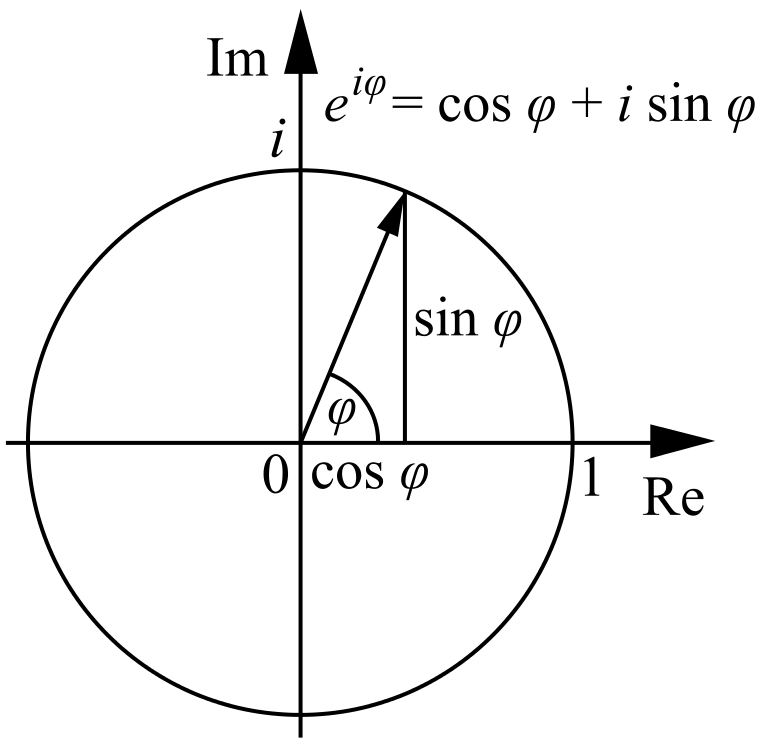
\includegraphics[width=0.5\textwidth]{Figures/eulersformula.png}
\caption{$e^{ix}$ traces a unit circle on the complex plane (\cite{eulerformula}).}
\label{fig:eulersformula}
\end{figure}

\section{Integral Transforms}

Integral transforms are a technique for transforming a function in one domain to an equivalent function is another domain. It just so happens that some problems are more easily solved in one domain than the other.

\subsection{The Laplace Transform}

The Laplace transform is an integral transform defined as,

$$F(s) = \mathcal{L}\{f(t)\} = \int_{0}^{\infty} f(t)e^{-st}\mathop{dt}.$$

It is a more generalised transform than the Fourier transform, and maps a function, $f(t)$, from the time ($t$) domain to the $s$ domain. The inverse Laplace transform is a more complicated function and usually it is more practical to take inverse transforms from a reference table. For example, let $f(x) = \cos kt$, we first use a trick to convert it to a more amenable form,

\begin{align}
\cos(kt) &= \frac{1}{2}\cos(kt) + \frac{1}{2}i\sin(kt) + \frac{1}{2}\cos(kt) - \frac{1}{2}i\sin(kt) \notag \\
&= \frac{1}{2}(\cos(kt) + i\sin(kt)) + \frac{1}{2}(\cos(-kt) + i\sin(-kt)) \notag \\
&= \frac{1}{2}e^{kit} + \frac{1}{2}e^{-kit}. \notag
\end{align}

Then,

\begin{align}
\mathcal{L}\{\cos(kt)\} &= \int_{0}^{\infty} \frac{1}{2}e^{kit}e^{-st} \mathop{dx} + \int_{0}^{\infty} \frac{1}{2}e^{-kit}e^{-st} \mathop{dt} \notag \\
&= \int_{0}^{\infty} \frac{1}{2}e^{(-s + ki)t} \mathop{dx} + \int_{0}^{\infty} \frac{1}{2}e^{(-s - ki)t}\mathop{dt} \notag \\
&= \frac{1/2}{s - ki} + \frac{1/2}{s + ki} = \frac{s}{s^2 + k^2}. \notag
\end{align}

If we are to apply the Laplace transform to differential equations, it is useful to establish a result for the transform of a derivative. By parts,

\begin{align}
\mathcal{L}\{f(t)\} = \int_{0}^{\infty} f(t)e^{-st}dt &= \Bigg[\frac{f(t)e^{-st}}{-s}\Bigg]_0^{\infty} - \int_{0}^{\infty} f'(t)\frac{e^{-st}}{-s}dt \notag \\
&= \frac{f(0)}{s} + \frac{1}{s}\mathcal{L}\{f'(t)\} \notag,
\end{align}

thus in general, $\mathcal{L}\{f^{(n)}(t)\} = s^n \mathcal{L}\{f(t)\} - s^{n-1}f(0) - \dots - f^{(n-1)}(0)$. Now, the linear homogeneous ordinary differential equation,

$$y'' - 5y' + 6y = 0,$$

with initial conditions $y(0) = 2$, and $y'(0) = 2$, can be solved with the Laplace transform. Using the derivatives formula on the left-hand side of the equation,

$$\mathcal{L}\{y\} - 5\mathcal{L}\{y'\} + 6\mathcal{L}\{y''\} = s^2\mathcal{L}\{y\} - 2s - 2 - 5s\mathcal{L}\{y\} +10 + 6\mathcal{L}\{y\},$$

from which we have,

$$\mathcal{L}\{y\} = \frac{2s - 8}{s^2 - 5s + 6} = \frac{4}{s - 2} - \frac{2}{s - 3},$$

hence $$y = \mathcal{L}^{-1}\bigg\{\frac{4}{s - 2}\bigg\} - \mathcal{L}^{1}\bigg\{\frac{-2}{s - 3}\bigg\} = 4e^{2t} - 2e^{3t}.$$

\subsection{Fourier Series}

A Fourier series, $g(t)$, is a way of representing any periodic function, $f(t)$, as the sum of a (possibly infinite) set of sines and cosines,

$$g(t) = \sum_{n=0}^{\infty}a_n\cos\bigg(\frac{2\pi nt}{T}\bigg) + \sum_{m=1}^{\infty}b_m\sin\bigg(\frac{2\pi mt}{T}\bigg),$$

where $a_0$ is an offset term, and $T$ is the fundamental frequency, that is, the lowest value for which the function is periodic, that is, the lowest value for which $f(t + T) = f(t)$ for all $t$. Deriving a Fourier series representation involves solving for the $a_n$ and $a_m$ parameters. It is possible to isolate each parameter by multiplying by the corresponding wave and integrating over the fundamental frequency. This eliminates all other terms in the series leaving,

$$a_n = \frac{2}{T}\int_0^Tg(t)\cos\bigg(\frac{2\pi nt}{T}\bigg)\mathop{dt}.$$

A Fourier series can also be thought of as a technique for decomposing the harmonics of a wave. For example, a square wave function can be represented as an infinite sum of cosines, each higher frequency part converging asymptotically to the square wave form. A Fourier series is often written in terms of complex exponential function, as this is more elegant and often makes integration less cumbersome.

\subsection{The Fourier Transform}

Fourier transforms are widely used in statistics, engineering, and physics. The Fourier transform maps a function in the time domain to a function in the frequency domain. The Fourier transform is defined as,

$$\hat{f}(\xi) = \int_{-\infty}^{\infty}f(x)e^{-2\pi ix\xi}\mathop{dx},$$

and the inverse Fourier transform is defined as,

$$f(x) = \int_{-\infty}^{\infty}\hat{f}(x)e^{2\pi i\xi x}\mathop{d\xi}.$$

The initial function $f(x)$ is a function of amplitude over time. The transformed function gives the amplitude for a given frequency. For $f(x) = \sin(x)$, the transform becomes a Dirac delta function, that is, a single point on the real plane, corresponding to the single frequency of the function. A more complex sine wave, comprising multiple frequencies, will transform to a sum of delta functions, each representing a frequency. For the square wave function, composed of an infinite summation of frequencies, the transform takes the form $\hat{f}(\xi) = \text{sinc}(x) = \sin(x)/x$, a contiunous sine wave with ever decreasing amplitude. There is such a thing as a discrete Fourier transform (DFT) for signals with sampled discretely. The famous Shannon-Nyquist theorem relates continuous and discrete signals, proving that a sample rate of at least twice the highest frequency of the continuous wave is sufficient for an exact reproduction. The fast Fourier transform (FFT) is an important $\mathcal{O}(n\log n)$ time algorithm for evaluating a discrete Fourier transform.

\section{The Factorial Function}

The factorial function, written $n!$, for a positive integer $n$ is the product of all natural numbers less than or equal to n. That is, $$n! = n \times (n - 1) \times (n - 2) \times \cdots \times 1.$$ The value of $0!$ is 1, not as a matter of mathematical necessity, but because it continues the pattern: $0! = (n - n)! = n!/n! = 1$. Otherwise, we can note that the factorial function models the number of permutations of $n$ objects, that is, $^nP_n = n!$. The number of ways of permuting \emph{no} objects is assuredly 1, as no reorderings of \emph{no} objects are possible. There is also such a thing as the \emph{double} factorial function,

$$n!! = n \times (n - 2) \times (n - 4) \times \cdots,$$

which multiples all even numbers $\leq n$ if n is even, and all odd numbers $\leq n$ if n is odd.  The factorial function is undefined for non-natural numbers, but the gamma function extends it to all real and complex numbers. The factorial function grows faster than exponentiation, but not as fast as double exponentiation or tetration, the hyperoperation of repeated exponentiation. That is,

$$\mathcal{O}(a^x) < \mathcal{O}(x!) < \mathcal{O}(a^{b^x}) < \mathcal{O}(^nx = x^{x^{\iddots^{x}}})$$

\subsection{Stirling's Approximation}

Stirling's approximation is a powerful approximation for the factorial function that converges as $n \to \infty$. It was first discovered by de Moivre, but Scottish mathematician James Stirling (1692-1770) found a nice simplification. Its derivation begins by taking the log of the factorial function,

$$\ln(n!) = \ln(1) + \ln(2) + \ln(3) + \cdots + \ln(n).$$

Now we notice that subtracting $\frac{1}{2}(\ln(1) + \ln(n))$ gives the trapezoidal rule\footnote{The trapezoidal rule is a part of a family of techniques for approximating integrals known as Riemann sums.} approximation to the integral of $\ln(n)$ with $\Delta x = 1$. That is,

\begin{align}
\ln(n!) - \cancelto{0}{\frac{1}{2}\ln(1)} - \frac{1}{2}\ln(n) &= \frac{\cancelto{0}{\ln(1)} + \ln(2)}{2} + \frac{\ln(2) + \ln(3)}{2} + \frac{\ln(3) + \ln(4)}{2} \cdots + \frac{\ln(n + 1) + \ln(n)}{2} \notag \\
&\approx \int_{1}^{n} \ln{x} \mathop{dx} = n\ln n - n + 1 + \sum_{k=2}^{m} \frac{(-1)^kB_k}{k(k-1)}\Bigg(\frac{1}{n^{k-1}} - 1\Bigg) + R_{m,n}. \notag
\end{align}

The error term is expressed in terms of Bernoulli numbers, $B_k$ and the remainder term, $R_{m,n}$, from the Euler-Maclaurin formula. The index, $m$, may be chosen freely, with $R_{m, n} \to 0$ as $m \to \infty$. We next consider the behaviour of the error term as $n$ tends to $\infty$,

$$\lim_{n \to \infty}\Big(\ln(n!) - \frac{1}{2}\ln n - n\ln n + n\Big) = 1 - \sum_{k=2}^{m} \frac{(-1)^kB_k}{k(k-1)} + \lim_{n \to \infty}R_{m,n},$$

and it is known that $\lim_{n \to \infty}R_{m,n} = R_{m,n} + O\Big(\frac{1}{n^m}\Big)$. Thus, the difference tends toward a constant, denoted $c$. Returning to our equation, we have,

$$\ln(n!) = n\ln n - n + \frac{1}{2}\ln n + 1 + c + \sum_{k=2}^{m} \frac{(-1)^kB_k}{k(k-1)}\Bigg(\frac{1}{n^{k-1}}\Bigg) + \mathcal{O}\Bigg(\frac{1}{n^m}\Bigg).$$

To eliminate the bothersome sum, we can choose the parameter, $m = 1$, incurring an error term of greater magnitude, $O(1/n)$. Exponentiating both sides gives,

$$n! = e^c\cdot\Bigg(\frac{n}{e}\Bigg)^n \cdot \sqrt{n} \cdot \Bigg(1 + \mathcal{O}\Bigg(\frac{1}{n}\Bigg)\Bigg),$$

as $n \to \infty$. Note that the error term comes from the fact that $e^x \approx 1 + x$, for $x$ close to 0. To deal with the constant, $e^c$, which we will denote, $C$, recall from Wallis' product that,

$$\frac{1}{2n + 1} \cdot \frac{2^{4n}(n!)^4}{[(2n)!]^2} \to \frac{\pi}{2},$$

as $n \to \infty$. Substituting our convergent expression for $n!$,

$$\frac{1}{2n + 1} \cdot \frac{2^{4n}[C(n/e)^n\sqrt{n}]^4}{[C(2n/e)^{2n}\sqrt{2n}]^2} = \frac{n}{4n + 2}\cdot C^2 \to \frac{\pi}{2},$$

from which we can see $C \to \sqrt{2n}$, as $n \to \infty$. Finding the convergent value through application of Wallis' product was Sterling's contribution. Our approximation therefore simplifies to Sterling's approximation,

$$n! \to \sqrt{2\pi n}\Bigg(\frac{n}{e}\Bigg)^n.$$

\subsection{The Gamma Function}

The gamma function is a continuous function that interpolates the factorial function (Figure \ref{fig:factorial}), and extends its domain from the natural numbers to the real and complex numbers. It is defined as,

$$\Gamma(t) = \int_0^{\infty} x^{t-1}e^{-x}\mathop{dx}.$$

To show its connection to the factorial function, we integrate by parts,

\begin{align}
\Gamma(n) &= \big\{-x^{n-1}e^{-x}\big\}_{x=0}^{\infty} + (n - 1)\int_0^{\infty} x^{n-2}e^{-x}\mathop{dx} \notag \\
&= (n-1)\Gamma(n-1).\notag
\end{align}

Noting that $\Gamma(1) = 1$, it is clear that $\Gamma(n) = (n - 1)!$ for all positive integers, $n$. However, the gamma function is further defined for all complex numbers, $t$. It is worth nothing that there exists a related function, the pi function, $\Pi(t) = \Gamma(t + 1)$, that does away with the offset term, so as to coincide exactly with the factorial function. Another related function, the beta function, is a composite of the gamma function, where $B(x, y) = \Gamma(x)\Gamma(y)/\Gamma(x+y)$. The gamma function makes many appearances in the domain of statistics, for example in Student's t-distribution. There is also an intimate link to the Normal distribution, which we can show by first observing that the form of the function $\varphi(x) = e^{-x^2}$ is that of the bell curve. Now, the infinite integral\footnote{An integral taken over an infinite integral is known as \emph{improper} and is an abuse of notation to do away with limits.} of this function is,

$$\int_{-\infty}^{\infty} e^{-t^2} \mathop{dt} = 2\cdot\int_{0}^{\infty} e^{-t^2} \mathop{dt}.$$

Defining $t = u^{1/2}$, we have it that $\mathop{dt} = \frac{1}{2}u^{-1/2}\mathop{du}$ and integrating by substitution gives,

$$\int_{-\infty}^{\infty} e^{-t^2} \mathop{dt} = 2\cdot\frac{1}{2}\cdot\int_{0}^{\infty}u^{1/2 - 1} e^{-u}\mathop{du} = \Gamma(1/2).$$

Given that we know the area under the unnormalised bell curve to be $\sqrt{\pi}$, we may write, $\Gamma(1/2) = \sqrt{\pi}$. Though there exist many such identities for points on the gamma function, to evaluate the gamma function at any positive real point, the Stirling approximation was historically used as a good approximation. Its use has been supplanted in recent decades by the numerical algorithm, the Lanczos approximation. An interesting property of the gamma function is that it is the only function that interpolates the factorial function and is also log-convex. This is according to a result known as the Bohr-Mollerup theorem.

\begin{figure}[!ht]
\centering
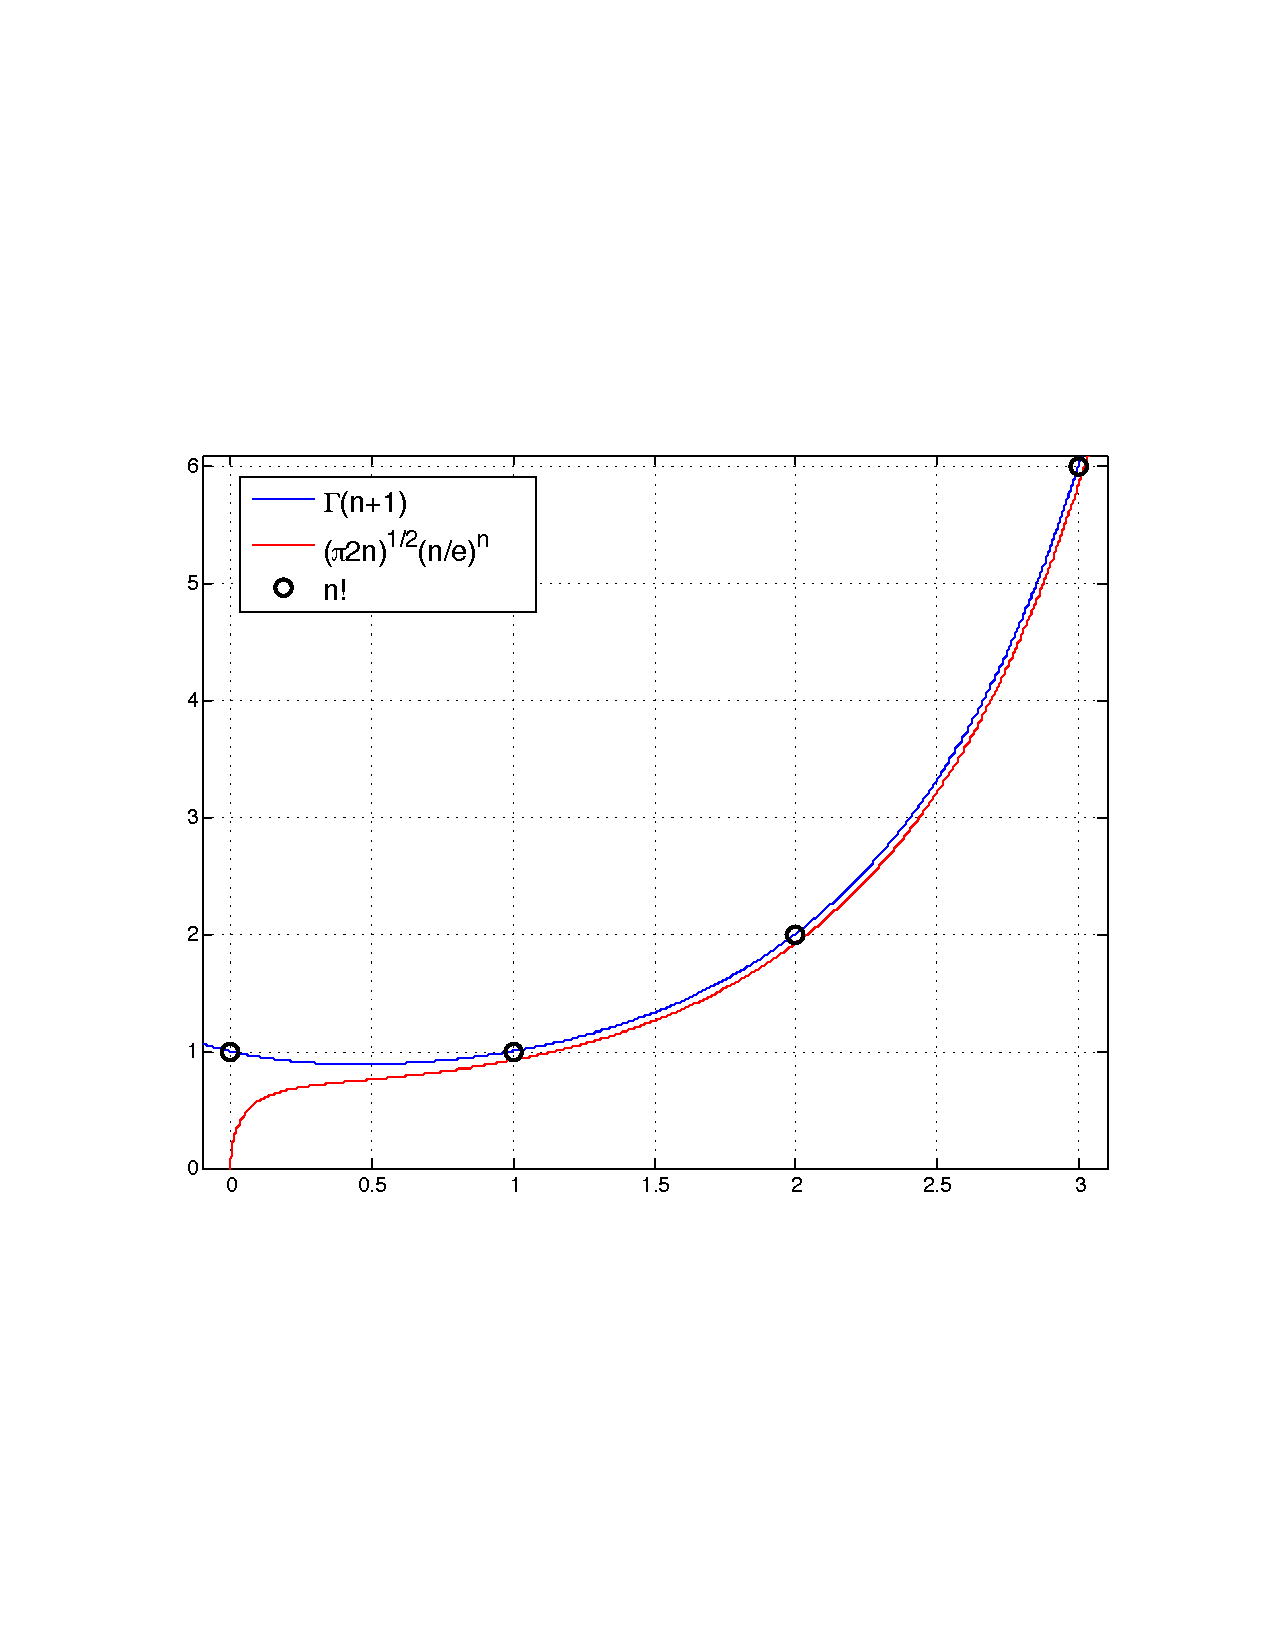
\includegraphics[width=0.6\textwidth]{Figures/factorial.pdf}
\caption{Comparison of the discrete factorial points, the gamma function, which interpolates them, and Stirling's approximation.}
\label{fig:factorial}
\end{figure}

\section{Fundamentals of Statistics}
\subsection{Philosophical Notions of Probability}

Pierre-Simon Laplace (1749-1827) described probability as, `nothing but common sense reduced to calculation.'\footnote{That is not to say probability theory is intuitive (it is often not), but rather that probabilities model real world phenomena in an intuitive, simplified way, without addressing the potentially complex physical interactions behind them. A good example is the central limit theorem and the bell curve, which smooths over the uncountable complexities of reality.} As it is, there are two competing interpretations of the meaning of probabilities: the \emph{frequentist} interpretation, and the \emph{Bayesian} interpretation. In the frequentist interpretation, probabilities represent frequencies or rates. Thus, a probability of $0.5$ that a coin comes up heads\footnote{Although recent research has shown the probability is slightly biased towards the upward-facing side of the coin when flipped, with about a $51\%$ chance of landing on that same side. This is linked somehow to the physics of the problem. See the Diaconis-Holmes-Montgomery coin-tossing theorem.} means that, with sufficient throws, this proportion of heads will prevail. In the Bayesian (or epistemological) interpretation, probabilities quantify an \emph{uncertainty} or \emph{degree of belief} in an outcome, and so is more closely aligned with information theory. In information theory, a fair coin flip (50-50) has maximum entropy, because a uniform distribution maximises uncertainty. Though both views are fully compatible, adopting one or the other may change the emphasis.

\subsection{Fundamental Rules}

\subsubsection{Probability Functions}

Probabilities express the uncertainty (or frequency) of a random variable, $X$, of assuming states (events) $A, B, C, \dots$, as a numeric value between 0 (impossible) and 1 (certain). A distribution may be defined by a function to allocate the probabilities. We write $p(X=A)$ or simply $p(A)$ for the probability $X$ assumes state $A$.

Discrete random variables take values in a finite or countably infinite set (such as the set of integers). The function that assigns each event a probability is called the probability mass function (pmf). The probabilities of events in a distribution must sum to 1. Thus,

$$\Bigg(\sum_{k = 1}^{K} p(X = k)\Bigg) = 1.$$

Continuous probability distributions express probabilities for random variables taking values in a continuum. For this reason, it no longer makes sense to model probabilities of the form $p(X = k)$. Such an event taken apart has an infinitesimal probability. Rather, we compute the probability of intervals, such as $p(X \leq k)$. The function that assigns probabilities is the cumulative density function (cdf),

$$
P(X \leq a) = \int_{-\infty}^{a} p(x) \mathop{dx}.
$$

Should we wish to compute the probability of a closed interval, we take,

$$P(a \leq X \leq b) = P(X \leq b) - P(X \leq a).$$

The cdf is the integral of the \emph{probability density function} (pdf), written $p(x)$, a function that expresses \emph{densities}. A density is a quantity related to probability by the expression, $P(x \leq X \leq x+dx) \approx p(x)dx$, so that the value of $p(x)$ can be though of as the relative weight of probabilities measured on intervals local to $x$. In actual fact, the pdf is the derivative of the cdf with,

$$p(x) = \lim_{\Delta x \to 0} \frac{P(x + \Delta x) - P(x)}{\Delta x},$$

and for this reason, the pdf must be non-negative, and must integrate to $1$.

\subsubsection{Union of Events}

The probability of a union of events $A$ and $B$, that is, the probability that $A$ \emph{or} $B$ occurs is, $$p(A \lor B) = p(A) + p(B) - p(A \land B).$$ When $A$ and $B$ are \emph{mutually exclusive}, the joint probability, $p(A \land B) = 0$. Mutually exclusive events are events that cannot happen simultaneously, such as $A$, the event of rolling a 2 on a die, and $B$, the event of rolling a 3 on a die. An example of events that are \emph{not} mutually exclusive is $A$, the event we draw a king from a deck of cards, and $B$, the event we draw a diamond. The events can happen either separately or together. Measuring the probability of the union of events seems rarely to be of interest in machine learning, however.

\subsubsection{Inclusion-Exclusion Principle}

The generalisation to the union of events formula is arrived at using the inclusion-exclusion principle, used for counting unions of sets. The case corresponding to the probability of the union of two events stated above is,

$$|A \cup B| = |A| + |B| - |A \cap B|,$$

for sets $A$ and $B$. If we include a third set, $C$, we acquire,

$$|A \cup B \cup C| = |A| + |B| + |C| - |A \cap B| - |A \cap C| - |B \cap C| + |A \cap B \cap C|,$$

These ideas are most easily understand by looking at Venn diagrams (Figure \ref{fig:inclusionexclusion}), where the probability spaces of the events are depicted as sets. In general, the probability of the union of $n$ events is,

$$p(X_1 \lor \dots \lor X_N) = \sum_{i = 1}^{N}p(X_i) - \sum_{1 \leq i < j \leq N}p(X_i \land X_j) + \sum_{1 \leq i < j < k \leq N}p(X_i \land X_i \land X_j) - \cdots + (-1)^{N-1}p(X_1 \land \dots \land X_N)$$

\begin{figure}[!ht]
\centering
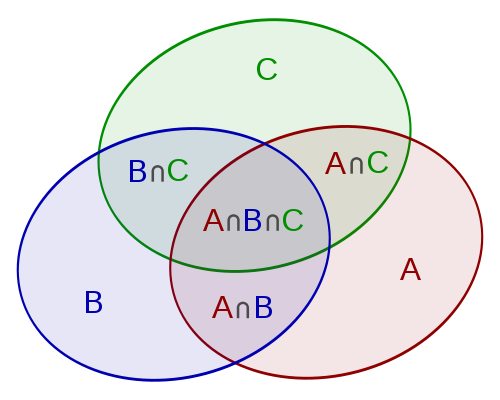
\includegraphics[width=0.5\textwidth]{Figures/inclusionexclusion.png}
\caption{The inclusion-exclusion principle is best understood with Venn diagrams (\cite{inclusionexclusion}).}
\label{fig:inclusionexclusion}
\end{figure}

\subsubsection{Intersection of Events}

The joint distribution, $p(A \land B)$, or simply, $p(A, B)$, is the probability that events $A$ and $B$ occur together. The joint distribution is factorised in accordance with the dependencies of the events. If two events, $A$ and $B$, are independent, we write $A \indep B$. Independence is distinct from mutual exclusivity, which is exclusive or. Independent events may occur apart or together, but the essence of independence is that the occurrence of one event does not affect the occurrence of the other. Hence, the joint distribution of independent $A$ and $B$ is,

$$p(A, B) = p(A)p(B),$$

that is, the product of the probabilities of the events taken separately. When $A$ and $B$ are \emph{dependent}, the occurrence of one changes the probability of the other occurring. In this case we write,

\begin{align}
p(A, B) &= p(A|B)p(B) \label{eq:condition1} \\
&= p(B|A)p(A). \label{eq:condition2}
\end{align}

The probability, $p(A|B)$, is the conditional probability of the event $A$ \emph{given} the occurrence of event $B$. Notice the symmetry of the conditioning--we can condition on any variable we like. The definition of independence is that $p(A|B) = p(A)$.

\subsection{Bayes' Theorem}

We may derive the all-important Bayes' theorem by equating equations (\ref{eq:condition1}) and (\ref{eq:condition2}) and rearranging,

$$p(A | B) = \frac{p(B | A)p(A)}{p(B)}.$$

Bayesians interpret this as an expression relating event $A$ and evidence $B$. The probability $p(A)$ is known as the `prior' distribution for the event taken alone (that is, `before' the evidence is presented). The `posterior' distribution, $p(A | B)$, represents the change in the uncertainty of the event after the evidence of the likelihood, $p(B | A)$, has been presented.

\subsubsection{Chain Rule}

Extending the intersection rule gives us a general result for $N$ random variables, $X_!, X_2, \dots, X_N$, known as the chain rule. The joint distribution may be factorised,

\begin{align}
p(X_1, X_2, X_3,\dots,X_N) &= p(X_1)p(X_2, X_3, \dots, X_N|X_1) \notag \\
&= p(X_1)p(X_2|X_1)P(X_3, \dots, X_N|X_1, X_2) \notag \\
&= p(X_1)p(X_2|X_1)P(X_3|X_1, X_2)\cdots P(X_N|X_1, X_2, \dots, X_{N-1}) \notag
\end{align}

\subsubsection{Law of Total Probability}

The law of total probability allows us to calculate the probability of an event by summing over a joint distribution,

\begin{align}
p(X=x) &= \sum_{y \in Y} p(X=x, Y=y) \notag \\
&= \sum_{y \in Y} p(X=x|Y=y)p(Y=y). \notag
\end{align}

This is called the marginal distribution on $X$, and we say that $Y$ has been `marginalised out'.

\subsubsection{Markov Chain}
A Markov chain is a sequence of random variables, $X_1, X_2, \dots, X_N$ written,

$$X_1 - X_2 - \cdots - X_N.$$

A Markov chain exhibits the Markov property, meaning each variable is dependent only on the previous variable in the sequence. Otherwise put, $p(X_{N+1}|X_N, X_{N-1}) = p(X_{N+1}|X_N)$. The chain rule applied to a Markov chain therefore simplifies to,

\begin{align}
p(X_1, X_2, X_3,\dots,X_N) &= p(X_1)p(X_2|X_1)P(X_3|X_1, X_2)\cdots P(X_N|X_1, X_2, \dots, X_{N-1}) \notag \\
 &= p(X_1)p(X_2|X_1)P(X_3|X_2)\cdots P(X_N|X_{N-1}) \notag
\end{align}

To give an example of what a Markov chain might model, let $X$ be the event that we see clouds on the horizon this morning; $Y$ it is raining by noon; $Z$ it is raining this evening. These events form a Markov chain, $X-Y-Z$. The probability of rain at noon, $Y$, is clearly dependent on there being clouds in the morning, $X$. That it rains in the evening, $Z$, also depends on there being clouds in the morning, $X$, but not once we have knowledge of $Y$. Thus, $Z$ is independent of $X$ given (conditioned on) the more recent and informative event $Y$.

\subsection{Quantiles}

Quantiles mark milestones in the cumulative distribution, that is, the values for which certain cumulative probabilities are reached. Quantiles may be taken anywhere, but the most common ones are:

\begin{itemize}
\item median - the value for which there is a 0.5 probability of exceeding and 0.5 probability of falling short, that is, the midpoint of the distribution;
\item quartile ($Q_1, Q_2, Q_3$) - the values marking 0.25, 0.5, and 0.75, probabilities in the cumulative distribution ($Q_2$ is the median). Note that in certain fields that apply statistics, such as finance, a quartile is rather one of the four intervals separated by the quartile points;
\item percentile - the values marking the $0.01, 0.02, \dots, 0.99$ cumulative probabilities.
\end{itemize}

For a continuous distribution, any quartile, $q$, can be computed by solving the integral, for the desired probability,

$$
p = \int_{-\infty}^{q} p(x) \mathop{dx}.
$$


\subsection{Moments}

Moments are quantitative measures (statistics) of a distribution first formulated by English statistician Karl Pearson (1857-1936). The general form is,

$$
\mathbb{E}[(X - c)^N],
$$

for some constants, $c$ and $N$. When $c = 0$, we have what is called the \emph{raw} moment. Usually $c = \mathbb{E}[X]$, as we are chiefly interested in how $X$ moves about its mean, and these are called \emph{central} moments. Further, standardised moments are normally used in higher orders, presumably to moderate the exaggeration of higher powers.

\subsubsection{Expected Value}

The expected value (or mean, or average), denoted $\mu$, of a discrete random variable is the average of the random variable, weighted by its probabilities. It is the first-order ($N=1$) \emph{raw} moment (the central moment is 0 by definition). It is defined as,

$$
\mathbb{E}[X] \triangleq \sum_{x} p(x)\cdot x.\\
$$

Similarly, for continuous, $X$,

$$
\mathbb{E}[X] \triangleq \int_{-\infty}^{\infty} p(x) x \mathop{dx}.\\
$$ 

In general, the expectation of a transformation, $f(X)$, is $\mathbb{E}[f(X)] = \sum_x p(x)f(x)$

\subsubsection{Variance}

Variance, $\text{Var}[X]$, or $\sigma^2$, is the expected (average) squared deviation from the mean, and therefore a measure of spread. Clearly, we need a second order measure to indicate spread since the first moment will be 0 for a symmetric distribution (the negative scores cancelling out the positive scores). Thus, variance,

\begin{align}
\text{Var}[X] &= \mathbb{E}[(X - \mathbb{E}[X])^2] \notag \\
&= \mathbb{E}[X^2 - 2\mathbb{E}[X]X + \mathbb{E}[X]^2] \notag \\
&= \mathbb{E}[X^2] - 2\mathbb{E}[X]^2 + \mathbb{E}[X]^2 \notag \\
&= \mathbb{E}[X^2] - \mathbb{E}[X]^2. \notag
\end{align}

Another measure of spread is the standard deviation, $\sigma$, defined as the square root of the variance, $\sqrt{\sigma^2}$.

\subsubsection{Skewness}

Skewenss, $\gamma_1$, is the third order \emph{standardised} moment. It is a measure of the skew or \emph{asymmetry} of a distribution, and is simply the standardised third order central moment,

$$
\gamma_1 = \mathbb{E}\Bigg[\frac{(X - \mathbb{E}[X])^3}{\sigma^3}\Bigg]
$$

\subsubsection{Kurtosis}

Kurtosis, $\text{Kurt}[X]$, is the fourth-order standardised central moment. It is a measure of the heaviness of the tails of the distribution. It is defined to be,

$$
\text{Kurt}[X] = \frac{\mathbb{E}[(X - \mathbb{E}[X])^4]}{\mathbb{E}[(X - \mathbb{E}[X])^2]^2}
$$

\subsection{Sample Statistics}

Given a set of sample data $x_1, x_2, \dots, x_N$, we can compute estimates of the distribution's statistics. Samples are drawn at random \emph{with} replacement. The sample mean is simply the arithmetic average,

$$\bar{x} = \frac{1}{N}\sum_{i=1}^N x_i.$$

At first it may appear that through the $\frac{1}{N}$ term that we are assuming a uniform distribution. This is not the case, however. Wherever non-uniformity exists, the data will promote the right proportions as a matter of course, by supplying more likely scores in greater number. That is, the higher probabilities will feature more heavily, and receive more weight, effecting higher probabilities. The sample variance is a lot more curious. We might take the sample variance in a similar way to the mean,

$$\sigma_x^2 = \frac{1}{N}\sum_{i=1}^N (x_i - \bar{x})^2$$

This would be, surprisingly, not quite correct. This is due to the fact we are using the sample mean only, not the true mean. Given all possible samples, the expectation of the sample variance is,

\begin{align}
\mathbb{E}[\sigma_x^2] &= \mathbb{E}\Bigg[\frac{1}{N}\sum_{i=1}^N\Bigg(x_i - \frac{1}{N}\sum_{i=1}^N x_i\Bigg)^2 \Bigg] \notag \\
&=\frac{1}{N}\sum_{i=1}^N\mathbb{E}\Bigg[x_i^2 - \frac{2}{N}x_i\sum_{j=1}^N x_j + \frac{1}{N^2}\sum_{j=1}^N x_j \sum_{k=1}^N x_k\Bigg] \notag \\
&=\frac{1}{N}\sum_{i=1}^N\mathbb{E}\Bigg[\frac{N-2}{N}\mathbb{E}[x_i^2] - \frac{2}{N}\sum_{j\neq i}^N \mathbb{E}[x_ix_j] + \frac{1}{N^2}\sum_{j=1}^N \sum_{k\neq j}^N \mathbb{E}[x_jx_k] + \frac{1}{N^2}\sum_{j=1}^N \mathbb{E}[x_j^2]\Bigg] \notag \\
&=\frac{1}{N}\sum_{i=1}^N\mathbb{E}\Bigg[\frac{N-2}{N}(\sigma^2 + \mu^2) - \frac{2(N - 1)}{N} \mu^2 + \frac{N(N-1)}{N^2} \mu^2 + \frac{1}{N} (\sigma^2 + \mu^2)\Bigg] \notag \\
&= \frac{N-1}{N}\sigma^2, \notag
\end{align}

where $\sigma^2$ and $\mu$ are the true variance and mean. Note the substitution in the second to last step comes from the definition of variance, $\text{Var}[X] = \mathbb{E}[X^2] - \mathbb{E}[X]^2$. Thus, our formula becomes,

$$\sigma_x^2 = \frac{1}{N-1}\sum_{i=1}^N (x_i - \bar{x})^2.$$

This is called the unbiased sample variance, and the leading quotient is known as Bessel's\footnote{Friedrich Bessel (1784-1846) was a German mathematician and scientist.} correction. This formula is usually presented without the above justification, and may be baffling to the student. The same correction is used for the sample covariance and other statistics. Given independent samples, these statistics converge to the true statistics as the sample size increases, as per the law of large numbers. That is, the sample variance converges to the expected sample variance, and the Bessel's correction converges to 1.

\subsection{Covariance}

Covariance measures the interaction between random variables, that is, it quantifies how much two random variables move together. It is defined as,

\begin{align}
\text{Cov}[X, Y] &= \mathbb{E}[(X - \mathbb{E}[X])(Y - \mathbb{E}[Y])] \notag \\
&= \mathbb{E}[X^2 - \mathbb{E}[Y]X - \mathbb{E}[X]Y + \mathbb{E}[X]\mathbb{E}[Y]] \notag \\
&= \mathbb{E}[XY] - \mathbb{E}[X]\mathbb{E}[Y]. \notag
\end{align}

In the multivariate case, we have the covariance matrix as the outer product,

\begin{align}
\text{Cov}[\mathbf{x}] &\triangleq \mathbb{E}[(\mathbf{x} - \mathbb{E}[\mathbf{x}])(\mathbf{x} - \mathbb{E}[\mathbf{x}])^T] \notag \\
&= \begin{bmatrix}
\text{Var}[X_1] & \text{Cov}[X_1, X_2] & \dots & \text{Cov}[X_1, X_n] \\
\text{Cov}[X_2, X_1] & \text{Var}[X_2] & \dots & \text{Cov}[X_2, X_n] \\
\vdots & \vdots & \ddots & \vdots \\
\text{Cov}[X_n, X_1] & \text{Cov}[X_n, X_2] &\dots & \text{Var}[X_n]
\end{bmatrix} \notag
\end{align}

\subsection{Correlation}

Correlation is covariance normalised by the variance of each of the variables taken apart. It measures the extent to which two variables are \emph{linearly} related and computes a correlation coefficient in the range $[-1, 1]$. A correlation coefficient of 0 indicates no relation. The formula for correlation is,

$$\text{corr}(X, Y) = \frac{\text{Cov}[X, Y]}{\sqrt{\text{Var}[X]\text{Var}[Y]}}.$$

Similary, for the multivariate case, the correlation matrix is,

$$
\text{Corr}[\mathbf{x}] = \begin{bmatrix}
\text{Corr}[X_1, X_1] & \text{Corr}[X_1, X_2] & \dots & \text{Corr}[X_1, X_n] \\
\text{Corr}[X_2, X_1] & \text{Corr}[X_2, X_2] & \dots & \text{Corr}[X_2, X_n] \\
\vdots & \vdots & \ddots & \vdots \\
\text{Corr}[X_n, X_1] & \text{Corr}[X_n, X_2] &\dots & \text{Corr}[X_n, X_n]
\end{bmatrix}. \notag
$$

Each of the diagonal elements of the correlation matrix will be equal to 1.

\subsection{Transformation of Random Variables}

For random variable, $X$, define a new random variable, $Y = aX + b$. How have its properties changed? Recall for discrete variables that $\mathbb{E}[f(X)] = \sum_x p(x)f(x)$. Then we have,

\begin{align}
\mathbb{E}[X] &= \sum_x p(x)(ax + b) \notag \\
&= a\sum_x p(x)x + b\sum_x 1 = a\mathbb{E}[X] + b. \notag
\end{align}

The same result is arrived at for continuous random variables. This effect is known as the `linearity of expectation'. Variance behaves a little differently,

\begin{align}
\text{Var}[X] &= \mathbb{E}[(X - \mathbb{E}[X])^2] \notag \\
&= \mathbb{E}[(aX + b - (a\mathbb{E}[X] + b))^2] \notag \\
&= \mathbb{E}[a^2(X  - \mathbb{E}[X])^2] \notag \\
&= a^2\text{Var}[X] \notag
\end{align}

Thus, adding a constant to a random variable does not change its variance, but scaling a random variable scales its variance by the square of that factor.

\subsection{Change of Variables}

In the general case, given transformation, $Y = f(X)$, a discrete distribution can be derived by,

$$p_y(y) = \sum_{x:f(x)=y} p_x(x),$$

that is, by mapping the probabilities of the values of x corresponding to y via the mapping. Things are not so simple for continuous random variables, in which case we must address the cdf. Being a cumulative function, it is monotonic\footnote{A monotonic function holds the property that $f(b) > f(a)$ for any $b > a$.}. If it is monotonic, it is bijective\footnote{If $f$ is bijective, it is a one-to-one mapping.}, and if it is bijective, it is invertible. Therefore, we can write the cumulative distribution,

$$P_y(y) = P(f(X) \leq y) = P(X \leq f^{-1}(y)) = P_x(f^{-1}(y))$$

Now,

$$
p_y(y) \triangleq \frac{d}{dy}P_y(y) = \frac{d}{dy}P_x(f^{-1}(y)) = \frac{dx}{dy}\frac{d}{dx}P_x(x),
$$

giving us the \emph{change of variables} formula,

$$p_y(y) = p_x(x)\Big|\frac{dx}{dy}\Big|.$$

An example here would perhaps be useful, so let $X \sim U(-1, 1)$ and $Y = X^2$. Since X is uniformly distributed on an interval of length 2, its pdf, $p_x(x) = 1/2$. Therefore, by the change of variables formula, $p_y(y) = \frac{1}{2} \cdot \frac{1}{2}y^{-1/2} = \frac{1}{4}y^{-1/2}$.

In the multivariate case, we have need of the Jacobian matrix from vector calculus, and the change of variables formula becomes,

% that is, the matrix of partial derivatives\footnote{Not to be confused with the Hessian, which is the matrix of partial \emph{second} derivatives.}, defined as,
%
%$$\mathbf{J}_{\mathbf{x} \to \mathbf{y}} \triangleq \frac{\partial(y_1, \dots, y_n)}{\partial(x_1, \dots, x_n)} \triangleq 
%\begin{bmatrix}
%\frac{\partial y_1}{\partial x_1} & \dots & \frac{\partial y_1}{\partial x_n} \\
%\vdots & \ddots & \vdots \\
%\frac{\partial y_n}{\partial x_1} & \dots & \frac{\partial y_n}{\partial x_n} \\
%\end{bmatrix},
%$$
%
%and the change of variables formula becomes,

$$p_y(\mathbf{y}) = p_x(\mathbf{x})\big|\det \Bigg(\frac{\partial\mathbf{x}}{\partial\mathbf{y}}\Bigg)\big| = p_x(\mathbf{x})|\det \mathbf{J}_{\mathbf{y} \to \mathbf{x}}|.$$

\subsection{Monte Carlo Statistics}

Monte Carlo statistics are a branch of numerical techniques for providing estimations using random sampling. The name comes from the famous casino in the city in the principality of Monaco near the south of France. One famous example of applying Monte Carlo techniques is that of sampling from a unit circle inscribed inside a $2 \times 2$ unit square. The ratio of the areas of circle to square is $\pi : 4$. We can therefore estimate the value of $\pi$ by randomly sampling points within the square, and comparing the number of points that fall inside and outside the circle (Figure \ref{fig:montecarlo}). A sufficiently large sample would converge to the correct result by the law of large numbers.

\begin{figure}[!ht]
\centering
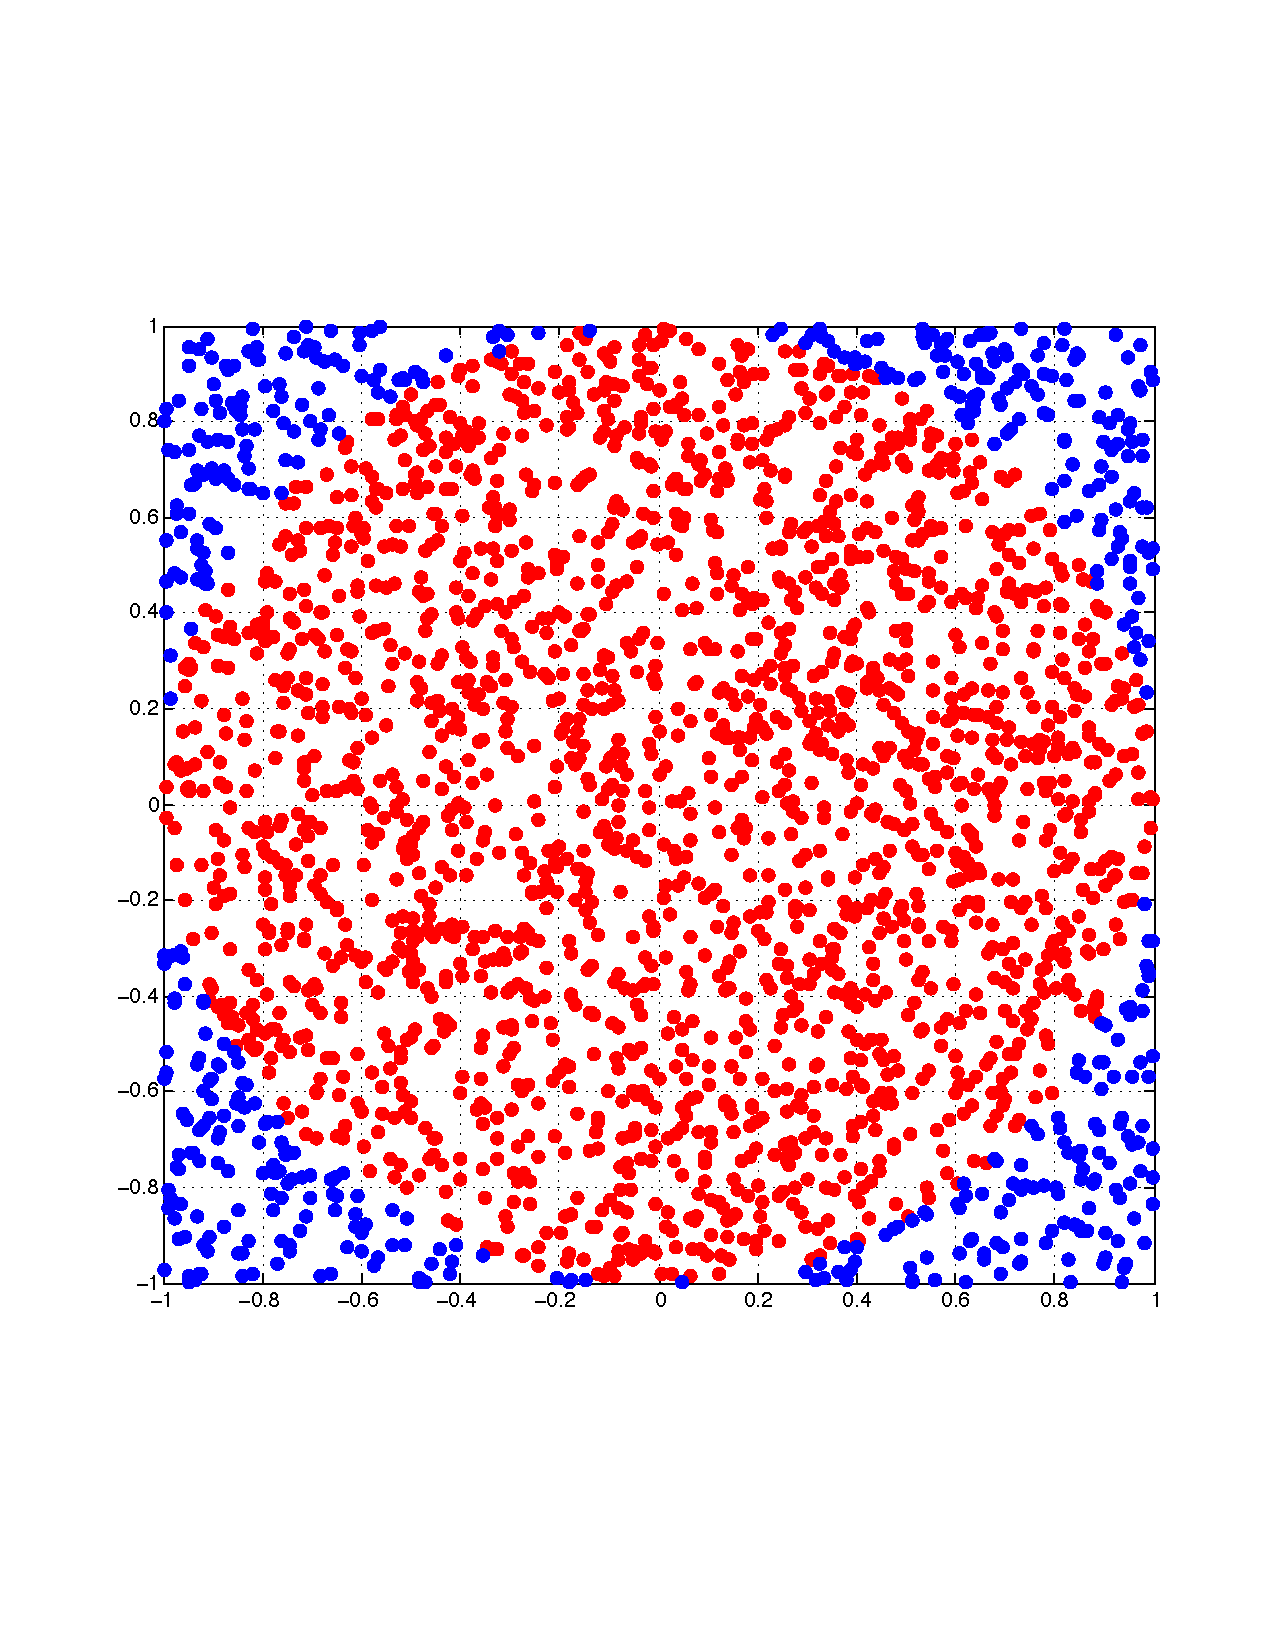
\includegraphics[width=0.5\textwidth]{Figures/montecarlo.pdf}
\caption{Monte Carlo approach to estimating $\pi$. 1963 of the 2500 random points landed in the circle, giving an estimation of $\pi \approx 3.1408$. Generated with \texttt{monteCarloDemo.m}.}
\label{fig:montecarlo}
\end{figure}

\subsubsection{Buffon's Needles}
An extremely nice and demonstrative Monte Carlo problem is know as the Buffon's needle problem. It also derives a technique for numerically computing the digits of $\pi$ using probabilities, but without invoking any circles explicitly. The problem consists of a set of parallel lines, separated by a distance of $2L$, where L is the length of each of the needles. The needles are then scattered randomly between the parallel lines. The proportion of needles intersecting a line gives us an approximation of $\pi$! There are two random variables at play here: the distance, $x$, of a needle from the nearest line; and the orientation, $\theta$, of the needle with respect to the lines. The assumption we make is that these are uniformly randomly distributed, hence $x$, which varies between 0 and $L$, has probability function $p_x = 1/L$, and $\theta$, which varies between $0$, $p_{\theta} = 2/\pi$. To determine the probability of a needle crossing a line, we note that it is sufficient that $x < \frac{L}{2}\sin\theta$. This is most easily seen with a diagram. These conditions alone are enough to calculate the probability,

$$
p = \int_{0}^{\pi/2}\int_{0}^{\frac{L}{2}\sin\theta}p_xp_{\theta}\mathop{dx}\mathop{d\theta} = \frac{2}{L\pi}\int_{0}^{\pi/2}\frac{L}{2}\sin\theta\mathop{d\theta} = \frac{1}{\pi}.
$$

Therefore, the proportion of a sample of $n$ scattered needles crossing a line gives, $\frac{\text{\# crosses}}{n} \approx \frac{1}{\pi} \implies \pi \approx \frac{n}{\text{\# crosses}}$

\section{Common Discrete Probability Distributions}

\subsection{Uniform Distribution}

A uniform distribution models a coin toss, or a die roll, or any other probability of $K$ events with equal chance, defining an interval, $[a, b]$, on some ordered encoding of the events. The probability mass function for a uniform distribution is,

$$p(k) = \frac{1}{K}.$$

The mean of this distribution is, $\mu = \frac{a + b}{2}$. Note there is also a continuous version of the uniform distribution. Laplace's \emph{principle of insufficient reason} argues to assume a uniform distribution for a discrete variable in the absence of further information (Gaussian for continuous variables).

\subsection{Bernoulli Distribution}

A Bernoulli distribution models an event with two alternative outcomes. It may therefore model a coin toss, but is parameterised with probability $\theta$ of outcome 1, and $1 - \theta$ of outcome 2. Thus, any binary event may be modelled. We write $X \sim \text{Ber}(\theta)$. Thus,

$$\text{Ber}(x|\theta) = \theta^{1_{x=1}}(1 - \theta)^{1_{x=0}}.$$

The expected value is therefore,

$$\mathbb{E}[X] = \theta \cdot 1 + (1 - \theta) \cdot 0 = \theta$$

\subsection{Binomial Distribution}

A Binomial distribution may model the number of heads, $k$, from the flipping of a coin (or any other binary event) $n$ times. The Binomial distribution generalises the Bernoulli distribution to $n$ binary trials (rather than a single trial). Its pmf is,

$$\text{Bin}(k | n,\theta) \triangleq {{n}\choose{k}}\theta^{k}(1 - \theta)^{n-k}$$

Note the resemblance in form to the Bernoulli distribution. The multinomial distribution further generalises the binomial distribution to $k$-ary events $n$ times.

\section{Common Continuous Probability Distributions}

\subsection{Laplace Distribution}

The Laplace pdf resembles two opposing exponential functions that meet in the middle, and is written,

$$f(x ; \mu, b) = \frac{1}{2b}\exp\Bigg\{-\frac{|x - \mu|}{b}\Bigg\},$$

where $b$ is a normalising constant. This distribution is similar in form to the Gaussian distribution, but the exponent is linear, and so the log probability decreases linearly, whereas a Gaussian's `tails' decrease quadratically. Thus, we say the Laplace distribution has `heavy' tails. This has implications when we fit a distribution to data (such as in machine learning), where the Laplace distribution is less sensitive to outliers, as extreme events have higher probability in a Laplace distribution than in a Gaussian. One advantage is it is easily integrable, whereas the Gaussian has no closed-form solution, as we shall see. Integrating the pdf gives,

\begin{align}
F(x) &= \int_{-\infty}^{+\infty} \frac{1}{2b}\exp\Bigg\{-\frac{|x - \mu|}{b}\Bigg\}dx \notag \\
&= \int_{-\infty}^{\mu} \frac{1}{2b}\exp\Bigg\{\frac{x - \mu}{b}\Bigg\}\mathop{dx} + \int_{\mu}^{+\infty} \frac{1}{2b}\exp\Bigg\{\frac{\mu - x}{b}\Bigg\}\mathop{dx} \notag \\
&= \frac{1}{2}\Bigg[\exp\Bigg\{\frac{x - \mu}{b}\Bigg\}\Bigg]_{x=-\infty}^{x=\mu} + \frac{1}{2}\Bigg[\exp\Bigg\{\frac{\mu - x}{b}\Bigg\}\Bigg]_{x=\mu}^{x=+\infty} \notag \\
&= \frac{1}{2}(1 - -0) + \frac{1}{2}(0 - -1) \notag
= 1, \notag
\end{align}

which confirms its validity as a probability distribution.

\subsection{Gaussian Distribution}

The Gaussian or Normal distribution was first proposed by Karl Frederich Gauss (1777-1855) in 1809. In the same paper, he presented other fundamental tenets of statistics--the method of least squares (for fitting data with Gaussian error), and maximum likelihood estimation. The pdf of a Gaussian distribution is,

$$f(x;\mu, \sigma) = \frac{1}{\sigma\sqrt{2\pi}}\exp\Bigg\{\frac{-(x - \mu)^2}{2\sigma^2}\Bigg\}.$$

Its shape is the well-known bell curve, the distribution so often seen in real-world data (the profound central limit theorem offers an explanation for why that is). The cdf for a Gaussian distribution,

$$\Phi({z;\mu,\sigma^2}) = \int_{-\infty}^{x}\mathcal{N}(z | \mu, \sigma^2)\mathop{dz}. \notag$$

Defining $u = \frac{z - u}{\sqrt{2}\sigma}$, and so $du = dz/\sqrt{2}\sigma$, we can integrate by substitution,

\begin{align}
\Phi({z;\mu,\sigma^2}) &= \frac{1}{\sigma\sqrt{2\pi}}\int_{-\infty}^{\frac{z - \mu}{\sqrt{2}\sigma}} e^{-u^2} \sqrt{2}\sigma\mathop{du} \notag \\
&= \frac{1}{2}\Big[\text{erf}(u)\Big]_{u=-\infty}^{u=(z-\mu)/\sqrt{2}\sigma} \notag \\
&= \frac{1}{2}\Bigg(1 + \text{erf}\Bigg(\frac{z - u}{\sqrt{2}\sigma}\Bigg)\Bigg), \notag
\end{align}

where $\text{erf}(x) = \frac{2}{\sqrt{\pi}}\int_{0}^{x}e^{-t^2}\mathop{dt}$ is the error function. This is a dead-end for closed-form solutions, and we must have recourse to an infinite series. Substituting the Taylor expansion for $e^{-t^2}$,

\begin{align}
\text{erf}(x) &= \frac{2}{\sqrt{\pi}}\int_{0}^{x} \sum_{k=0}^{\infty} \frac{(-t^2)^k}{k!} \mathop{dt} \notag \\
%&= \frac{2}{\sqrt{\pi}}\int_{0}^{x} \sum_{k=0}^{\infty} \frac{(-1)^kt^{2k}}{k!} dt \notag \\
&= \frac{2}{\sqrt{\pi}}\sum_{k=0}^{\infty} \frac{(-1)^kx^{2k + 1}}{k!(2k + 1)}, \notag
\end{align}

giving us an infinite series for the error function. Thus, thanks to Taylor series, approximations to the Gaussian CDF can be computed by statistical software, and placed in those mysterious statistics tables with which every student of statistics is familiar.

\subsubsection{Standardisation}

The standard Normal distribution is a Normal distribution with mean $0$ and variance $1$, $\mathcal{N}(0, 1)$. It is possible to \emph{standardise} a random variable, $X \sim \mathcal{N}(\mu, \sigma^2)$, by first subtracting its mean, $\mu$ (which adjusts the mean to 0 without changing the variance), then dividing by its standard deviation, $\sigma$, (which does not change the mean but shrinks the variance from $\sigma^2$ to 1), yielding,

$$Z = \frac{X - \mu}{\sigma}.$$

Since these transformations do not change the type of distribution, and a Gaussian is uniquely defined by its mean and variance, the transformed random variable, $Z$, is distributed according to the standard normal distribution.

\subsection{Chi-squared Distribution}

The chi-squared ($\chi^2$) distribution expresses a probability distribution over the sums of squares of $k$ normally distributed random variables. That is, the distribution of $Y$ where $Y = X_1^2 + X_2^2 + \dots + X_k^2$ for $k$, and where the $X_i \sim \mathcal{N}(0, 1)$ are i.i.d\footnote{independent and identically distributed} random variables. Note that by the central limit theorem, the chi-squared distribution converges to a normal distribution as $k \to \infty$. We write $Y \sim \chi^2_k$ where $k$ is the number of variables in the sum, also known as the \emph{degrees of freedom}. When the random variable $Y$ takes on a value, that value is like the dial of radius of a $k$-dimensional sphere, where the $k$ random variables are free to vary. The chi-squared distribution is the basis of some common statistical tests, and is also crucial to the derivation of other distributions, such as Student's t-distribution. The pdf of a chi-squared distribution is,

$$p(y; k) = \frac{1}{2^{\frac{k}{2}}\Gamma\big(\frac{k}{2}\big)}y^{\frac{k}{2} - 1}e^{-\frac{y}{2}},$$

where the parameter, $k$, is the number of degrees of freedom (number of variables in the sum), and $\Gamma$ is the gamma function. In the unique case that $k = 2$, the expression simplifies to $p(y; 2) = \frac{1}{2}e^{-y/2}$. We take the time to derive the pdf of the chi-squared distribution, as it involves several of the topics we have covered already.

In the simplest case, $k = 1$, we have $Y = X^2$. Since $X$ is a standardised Gaussian variable, its square makes all previously negative values positive. The shape of the pdf is therefore something like a stretched half-bell curve. We can derive the pdf of the transformed variable using the change of variables formula. Because of the symmetry of the squared variable, we have, $f_Y(y) = 2f_X(f^{-1}(y))\Big|\Big(\frac{\mathop{dx}}{\mathop{dy}}\Big)\Big|$. Now, $X = \sqrt{Y}$, so $dx/dy = 1/2\cdot y^{-1/2} $. Hence,

$$f(y; 1) = 2\frac{1}{\sqrt{2\pi}}e^{-(\sqrt{y})^2/2}\frac{1}{2}y^{-1/2} = \frac{1}{\sqrt{2}\Gamma(1/2)}e^{-y/2}y^{-1/2},$$

where we recall that $\Gamma(1/2) = \sqrt{\pi}$. The $k$th order case may be derived with a more involved version of the same technique. In the general case, it becomes clear that the variable $Y$, is directly related to a k-dimensional sphere, with surface area, $S$, given by,

$$S = \frac{2\pi^{\frac{n}{2}}}{\Gamma(\frac{n}{2})}.$$

This is how the gamma function comes to be part of the function.

\subsection{Student's T-Distribution}

The Student's t-distribution has an interesting history. Student is a pseudonym for the English mathematician who designed it, William Sealy Gosset (1876-1937), unable to attribute his true name due to his employment as a statistician at the Guiness brewery in Dublin. According to Gosset, the t-distribution expresses a distribution of the value of the sample mean of a Gaussian variable given the true standard deviation of the samples is unknown. The probability density function is,

$$f(t) = \frac{\Gamma(\frac{\nu + 1}{2})}{\sqrt{\nu\pi}\Gamma(\frac{\nu}{2})}\Bigg(1 + \frac{t^2}{\nu}\Bigg)^{-\frac{\nu + 1}{2}},$$

where $\Gamma(v)$ is the gamma function, and $\nu$, the Greek letter \emph{nu}, are the degrees of freedom. The variable, $t = \frac{\hat{x} - \mu}{s/\sqrt{n}}$, where $\hat{x} = (x_1 + \cdots + x_n)/n$ is the sample mean, $\mu$ is the true mean, $s^2 = \frac{1}{N - 1}\sum_{i=1}^{n} (x_i - \hat{x})^2$ is the sample variance, and $n$ is the sample size. The degrees of freedom is therefore $\nu = n - 1$. Thus, the Student's t-distribution distributes $t$, the sample mean.

\section{Hypothesis Testing}

\subsection{Standard Error}

Standard error is the standard deviation of the sample mean, $\bar{X} = \frac{1}{n}(X_1 + X_2 + \cdots X_n)$ from $n$ independent samples, $X_1, X_2, \dots, X_n$, where the true standard deviation $\sigma$ is known. The total, $$T = X_1 + X_2 + \dots + X_n,$$ has variance, $\sigma_T^2 = n\sigma^2$. Then, the variance of $\bar{X} = T/n$ is therefore, $$\sigma_{\bar{X}}^2 = \frac{1}{n^2}n\sigma^2 = \sigma^2/n.$$ We write finally the standard error as, $$\text{SE}_{\bar{X}} = \sigma/\sqrt{n}.$$ Clearly as $n \to \infty$, the standard error goes to $0$, reflecting that the sample mean converges to the true mean. Note that in practice $\sigma$ must be approximated by the sample variance.

\subsection{Confidence Intervals}

A confidence interval is the interval, expressed in standard deviations, around a sample mean, $\bar{X}$, known to contain the true mean, $\mu$, to a desired degree of certainty. Because of the central limit theorem, we know the sum of n random variables is normally distributed, hence the sample mean also. The standard error statistic tells us the standard deviation of this distribution. Because the Normal cdf has no closed form, it must be computed numerically. In practice, it is necessary to have a lookup table of precomputed probabilities from a standard normal distribution. The value of our variable can then be normalised and the corresponding probability retrieved. In a standard Normal distribution, $Pr(Z \leq 1.96) = 0.9775$ (approximately), and due to symmetry, $Pr(Z \geq - 1.96) = 0.9775$. That is, $95\%$ of the distribution sits in the interval $[-1.96, 1.96]$. In other words, $Z$ has a 95\% chance of being within 1.96 standard deviations ($\sigma = 1$ when standardised) of the mean. Thus, we may solve for our own $95\%$ confidence interval by writing,

$$1.96 = \frac{\bar{X} - \mu}{\sigma}.$$

Rearranging gives,

$$\mu = [\bar{X} - 1.96\times\text{SE}, \bar{X} + 1.96\times\text{SE}],$$

which is the general form for a $95\%$ confidence interval. Confidence intervals of arbitrary size can be constructed by looking up the normalised value of the desired probability.

\subsection{Hypothesis Testing}

We can use our knowledge of statistics to perform tests on sample data. The formal framework for this is to propose two hypotheses, one the null (or default) hypothesis, $H_0$, the other the alternative hypothesis, $H_1$. The procedure is to compute a statistic to challenge the statistical implications of the null hypothesis, producing a probability that the sample data is consistent with $H_0$. If the probability is lower than some conventional threshold (usually 0.05 or 0.1), $H_0$ is rejected and $H_1$ accepted, in a sort of probabilistic proof by contradiction. Erroneously rejecting $H_0$ is referred to as a type 1 error (false positive); erroneously accepting $H_0$ is referred to as a type 2 error (false negative).

\subsubsection{Z-test}

Many statistical tests exist, and perhaps the simplest is the $Z$-test, which can be used to decide whether a set of n samples conforms to a given distribution, by calculating the probability of the sample mean. The calculations are similar to creating a confidence interval, as it involves computing the SE and (implying the true mean and standard deviation be known) the Z-score, $Z = (\hat{X} - \mu)/\text{SE}$. The value of $Z$ is looked up in standard normal tables, yielding a probability. The probability (or p-value) is compared with a conventional threshold (typically 0.05 or 0.1) and the null hypothesis accepted or rejected depending on where it falls. We may interpret the Z-score as asking the question, `can this data reasonably be believed to have been drawn from our distribution?'

\subsubsection{Pearson's Chi-Squared Test}

This test checks for bias in categorical variables. The null hypothesis is that the $n$ categories of a variable are uniformly distributed. If, for example, we have a die producing a set of sample data from $N$ throws, we can compute the difference between the observed total of each category, $O_i$, $i = 1, \dots, 6$, and the expected total for a fair die, $E_i = \frac{1}{6}\times N$. This difference is assumed to be a continuous, normally distributed random variable. The normalised squared error for each variable is $(O_i - E_i)^2/E_i$. We can therefore sum these squared errors and use a chi-squared distribution with $k = 5$ degrees of freedom\footnote{In such problems, the degrees of freedom is $n - 1$, where $n$ is the number of categories. This is due to the fact that once the first $n-1$ variables are given, the final one is determined because the sum is constant.} to give us a probability for the null hypothesis.

\section{The Central Limit Theorem}
\subsection{Moment-Generating Functions}

The moment-generating function (MGF) of a random variable, $X$, is defined as,

\begin{align}
M_X(t) = \mathbb{E}[e^{tX}] &= \mathbb{E}\Bigg[\sum_{k = 0}^{\infty} \frac{(tX)^k}{k!}\Bigg] \notag \\
&= \sum_{k = 0}^{\infty} \frac{\mathbb{E}[X^k]t^k}{k!}. \notag
\end{align}

Such a function is an alternative specification of a distribution to a pdf. By L\'evy's continuity theorem, convergence in MGF implies convergence in distribution, a result that underpins the proof of the central limit theorem. The function is `moment-generating' in that the coefficients of the series expansion are the central moments of the distribution. The MGF of a \emph{sum} of $N$ i.i.d variables, $T = X_1 + X_2 + \cdots + X_N$ is,

\begin{align}
M_T(t) = \mathbb{E}[e^{tX_1 + tX_2 + \cdots + tX_N}] &= \mathbb{E}[e^{tX_1}]\mathbb{E} [e^{tX_2}] \cdots\mathbb{E}[e^{tX_N}] \notag \\
&= M_X(t)^N. \notag
\end{align}

The MGF of a Gaussian distribution\footnote{Here standardised for simplicity.} is,

$$M_z(t) = \mathbb{E}[e^{tZ}] = \int_{-\infty}^{+\infty}e^{zt}\frac{1}{\sqrt{2\pi}}e^{-z^2/2}\mathop{dz}.$$

If we consider the exponents, we have $e^{zt - z^2/2}$. Completing the square gives $e^{-z^2/2 + zt - t^2/2 + t^2/2} = e^{(z-t)^2/2}\cdot e^{t^2/2}$. Therefore we have,

\begin{align}
M_z(t) &= e^{t^2/2}\int_{-\infty}^{+\infty}\frac{1}{\sqrt{2\pi}}e^{(z-t)^2/2}\mathop{dz} \notag \\
&= e^{t^2/2} \cdot 1, \notag
\end{align}

since the integrated expression defines $\mathcal{N}(z ; t, 1)$. 

\subsection{Proof of the Central Limit Theorem}

The central limit theorem (CLT) is the crowning jewel of statistics--a profound result, with far-reaching applications. It explains, at least in part, the uncanny ubiquitousness of the bell curve in nature. Its proof is therefore the demonstration of a universal truth. This is where Laplace's statement that `probability is common sense reduced to calculation' resonates most strongly. The theorem states that the sum of $n$ random variables, whatever their individual distributions, converges to a Gaussian distribution as $n \to \infty$. If we then suppose natural phenomena to be aggregations of many random events, the central limit theorem explains how the bell curve appears with such regularity\footnote{A wonderful mechanical demonstration of the central limit theorem is the \emph{Galton board}. These can often be found in science museums.}.

Given $X_1, X_2, ... X_n$ are i.i.d. random variables with mean 0, variance $\sigma^2$, and moment-generating function, $M_x(t)$, denote their standardised sum, $Z = (X_1 + X_2 + \cdots X_n)/\sqrt{n\sigma^2}$. Therefore,

$$M_Z(t) = \Bigg(M_x\Bigg(\frac{t}{\sqrt{n\sigma^2}}\Bigg)\Bigg)^n.$$

A Taylor approximation for $M_x$ is,

$$M_x(s) = M_x(0) + sM_x(0) + \frac{1}{2}s^2M_x''(0) + o(s^2),$$

where $o(s^2)$ indicates a function that shrinks faster than a quadratic function as $s \to 0$. By definition, $M_x(0) = 0$, $M_x'(0) = 1$, and $M_x''(0) = \sigma^2$. Combining these results gives,

\begin{align}
M_Z(t) &= \Bigg(1 + \frac{t^2/2}{n} + o\Bigg(\frac{t^2}{n\sigma^2}\Bigg)\Bigg)^n \notag \\
&\to e^{t^2/2}, \ n \to \infty, \notag
\end{align}

that is, the MGF of a Normal distribution. Thus, the MGF, $M_Z(t)$, converges to the MGF of a Normal distribution. Hence, by the L\'evy continuity theorem, it converges in distribution to a Gaussian.

\section{The Law of Large Numbers}

In this section we prove one of the fundamental laws of statistics--the law of large numbers--first deriving the Markov and Chebyshev inequalities that are used in the proof.

\subsection{Markov Inequality}

The Markov inequality expresses a general property of probability distributions. An elegant proof exists, but it may be derived simply by the following observation: it is not possible for $(1/n)$th of a population to be greater than $n$ times the average value. Expressed mathematically this is,

$$\text{Pr}(X \geq a) \leq \frac{\mathbb{E}[X]}{a}$$

\subsection{Chebyshev Inequality}

The Chebyshev inequality is another general result for probabilities, expressing a bound on the probability of a random variable, $X$, straying from its mean, $\mu$, by more than $k$ standard deviations. To derive this, we first define a random variable, $Y = (X - \mu)^2$, and constant, $a = (k\sigma)^2$. Then, by the Markov inequality,

$$\text{Pr}((X - \mu)^2 \geq (k\sigma)^2) \leq \frac{\mathbb{E}[(X - \mu)^2]}{(k\sigma)^2},$$

which we may rewrite as,

\begin{align}
\text{Pr}(|X - \mu| \geq k\sigma) &\leq \frac{\text{Var}(X)}{k^2\sigma^2} \notag \\
&= \frac{1}{k^2} \notag
\end{align}

\subsection{Law of Large Numbers}

The law of large numbers states that given a sequence $X_1, X_2, \dots, X_N$ of i.i.d random variables, the sample average, $\bar{X} = \frac{1}{n}(X_1 + X_2 + \cdots + X_n)$ converges to the true mean, $\mu$, as n grows. That is, $\bar{X}_n \rightarrow \mu$ as $n \rightarrow \infty$.

Note first that,

\begin{align}
\text{Var}(\bar{X}_n) &= \text{Var}\bigg(\frac{X_1 + X_2 + \cdots + X_n}{n}\bigg) \notag \\
&= \frac{1}{n^2}\big(\text{Var}(X_1) + \text{Var}(X_2) + \cdots + \text{Var}(X_n)\big) \notag \\
%&= \frac{n\sigma^2}{n^2} \notag \\
&= \frac{\sigma^2}{n} \notag
\end{align}

Now, by the Chebyshev inequality,

$$
\text{Pr}(|\bar{X}_n - \mu| \geq k\frac{\sigma}{\sqrt{n}}) \leq \frac{1}{k^2}.
$$

Choosing $k = \frac{\sqrt{n}}{\sigma}\epsilon$ for any arbitrary choice of $\epsilon$,

$$
\text{Pr}(|\bar{X}_n - \mu| \geq \epsilon) \leq \frac{\sigma^2}{n\epsilon^2},
$$

that is,

$$
\text{Pr}(|\bar{X}_n - \mu| < \epsilon) \geq 1 - \frac{\sigma^2}{n\epsilon^2},
$$

which converges to 1 for a sufficiently large choice of $n$.

\section{Information Theory}

This section presents the basics of information theory.

\subsection{Entropy}

The entropy of a random variable, $X$, is a measure of its uncertainty. It is a core tenet of information theory, the science underpinning coding and signal processing. Entropy measures the average number of bits required to encode an alphabet, and is the lower bound on compression (coding). Entropy is defined as,

$$\mathcal{H}(X) = \sum_{x \in X}p(x)\log\frac{1}{p(x)}.$$

Entropy clearly must be positive, and is minimised for a distribution where a single event has probability 1, that is, a deterministic variable. In this case, the entropy of the variable is 0, that is, minimally uncertain. Hence, $\mathcal{H}(X) \geq 0$. When we have binary events, $x \in \{0, 1\}$, we have the binary entropy function, which simplifies to,

$$h_2(p) = -p\log p - (1-p)\log (1 - p).$$

\subsection{Kullback-Liebler Divergence}

Kullback-Liebler (KL) divergence is a measure of the disparity between two probability distributions, $p$ and $q$, written,

\begin{align}
\mathcal{D}(p || q) &= \sum_{k=1}^K p_k \log\frac{p_k}{q_k} \notag
\end{align}

KL divergence can therefore be interpreted as the average number of \emph{additional} bits required to encode an alphabet with chosen distribution $q$, given true distribution $p$. Like entropy, divergence must be greater than or equal to zero. To see this, write,

\begin{align}
-\mathcal{D}(p || q) &= -\sum_{k=1}^K p_k \log\frac{p_k}{q_k} \notag \\
&= \sum_{k=1}^K p_k \log\frac{q_k}{p_k} \notag \\
&\leq \log\Bigg(\sum_{k=1}^K p_k\frac{q_k}{p_k}\Bigg) \label{eq:jensen} \\
&= \log 1 = 0, \notag
\end{align}

where the inequality in (\ref{eq:jensen}) comes from applying Jensen's inequality, since $\log$ is a concave function. A corollary to this is that the distribution maximising entropy for discrete variables is the uniform distribution, since,

\begin{align}
0 \leq \mathcal{D}(p || u) &= \sum_{k=1}^K p_k \log\frac{p_k}{u_k} \notag \\
&= \sum_{k=1}^K p_k \log{p_k} - \sum_{k=1}^K p_k \log \frac{1}{K} \notag \\
&= -\mathcal{H}(p) + \log K \notag
\end{align}

\subsection{Mutual Information}

Mutual information uses the KL divergence to measure the difference in the entropy of a random variable, $X$, before and after a second variable, $Y$, (on which $X$ may be dependent) is introduced. The formula for mutual information is,

\begin{align}
I(X; Y) &\triangleq \mathcal{D}(p(X, Y) || p(X)p(Y)) = \sum_x \sum_y p(x, y) \log\frac{p(x, y)}{p(x)p(y)}\notag \\
&= \mathcal{H}(Y) - \mathcal{H}(Y|X) \notag \\
&= \mathcal{H}(X) - \mathcal{H}(X|Y) \notag,
\end{align}

and so it quantifies how much knowing about one variable tells us about the other (note the formula is symmetric). That is, how much uncertainty is lifted from $X$ by learning about $Y$, and vice versa. In other words, it measures \emph{the extent to which one random variable becomes deterministic once we learn about another}. For this reason, mutual information can be used as a more sophisticated correlation measure, as it may also reveal non-linear dependencies.

\section{Convex Optimisation}
\subsection{Convexity}
Convexity is a useful property in optimisation because it guarantees that any local optimum of a function is a \emph{global} optimum.

\subsubsection{Convex Sets}
A set of points, $S$, in a vector space is convex if for any two points $x_1$ and $x_2$ in $S$, all points in-between, that is, all points on the straight line connecting $x_1$ and $x_2$ are also in $S$. In a sense, it is a region that does not have any `holes'. For example, a circular region is convex, but a doughnut is not, nor is a crescent. A line passing through points $x_1$ and $x_2$ can be written, $x_1 + c(x_2 - x_1)$, for some constant $c$. Formally, a set $S$ is convex if,

$$S = \Big\{x_1, x_2 \in S \implies (1 - \lambda) x_1 + \lambda x_2 \in S \Big\},$$

for all $\lambda \in [0, 1]$, that is, all points along the chord between the two points are also part of the convex set. A convex hull of a set of points is the smallest convex region enclosing those points.

\subsubsection{Convex Functions}
A function, $f(x)$, is convex on an interval if,

$$
f((1 - \lambda)x_1 + \lambda x_2) \leq (1 - \lambda) f(x_1) + \lambda f(x_2),
$$

for all $\lambda \in [0, 1]$. That is, the curve lies below a line drawn between $x_1$ and $x_2$. A function with more than one turning point in a domain cannot be convex. Examples of convex functions are $e^x$, $x^2$, etc. \emph{Strict} convexity occurs when there is a strict inequality. \emph{Concavity} is the same property with the inequality reversed. Hence, $f(x)$ convex $\Longleftrightarrow$ $-f(x)$ concave. A linear function is both concave and convex.

\subsubsection{Jensen's Inequality}

Jensen's inequality essentially extrapolates the definition of convexity to $n$ dimensions, stating,

$$
f\Bigg(\sum_{i=1}^{N}\lambda_i \mathbf{x}_i\Bigg) = \sum_{i=1}^{N} \lambda_if(\mathbf{x}_i) \notag,
$$

for convex function, $f$, $\mathbf{x} \in \mathcal{R}^N$, and $\sum_{i=1}^N \lambda_i = 1$. For $N = 2$, we have,

$$
f(\lambda_1 x_1 + \lambda_2 x_2) \leq \lambda_1f(x_1) + \lambda_2f(x_2),
$$

for any $\lambda_1, \lambda_2$ such that $\lambda_1 + \lambda_2 = 1$ (definition of convexity). Then suppose, $f\big(\sum_{i=1}^k\lambda_i x_i\big) \leq \sum_{i=1}^k \lambda_if(x_i).$ We define,

$
\lambda_j = \begin{cases}
\ \ \ \ \lambda_i & j = 1: k-1 \\
\lambda_k + \lambda_{k+1} & j = k
\end{cases} $ and $
x_j = \begin{cases} 
\ \ \ \ \ \ \ \ \ \ \ \ \ \  x_i & j = 1: k-1 \\
\frac{\lambda_k}{\lambda_k + \lambda_{k+1}}x_k + \frac{\lambda_{k+1}}{\lambda_k + \lambda_{k+1}}x_{k+1} & j = k
\end{cases}$, then,

\begin{align}
f\Bigg(\sum_{i=1}^{k+1}\lambda_i x_i\Bigg) &= f\Bigg(\sum_{j=1}^{k}\lambda_j x_j\Bigg) \notag \\
&\leq \sum_{j=1}^k \lambda_jf(x_j) \notag \\
&= \sum_{i=1}^{k-1} \lambda_if(x_i) + (\lambda_k + \lambda_{k+1})f\Bigg(\frac{\lambda_k}{\lambda_k + \lambda_{k+1}}x_k + \frac{\lambda_{k+1}}{\lambda_k + \lambda_{k+1}}x_{k+1}\Bigg) \notag \\
&\leq \sum_{i=1}^{k-1} \lambda_if(x_i) + (\lambda_k + \lambda_{k+1})\frac{\lambda_k}{\lambda_k + \lambda_{k+1}}f(x_k)+ \frac{\lambda_{k+1}}{\lambda_k + \lambda_{k+1}}f(x_{k+1}) \notag \\
&= \sum_{i=1}^{k+1} \lambda_if(x_i) \notag, 
\end{align}

and Jensen's inequality follows from the principle of mathematical induction.

\subsubsection{Sums of Convex Functions}
An important result is that if we sum two convex functions, the result is convex also. To see this in two dimensions, define convex functions $f(x)$ and $g(x)$, and their sum $h(x)$. Then,

\begin{align}
h((1 - \lambda)x_1 + \lambda x_2) &= f((1 - \lambda)x_1 + \lambda x_2) + g((1 - \lambda)x_1 + \lambda x_2) \notag \\
&\leq (1 - \lambda)f(x_1) + \lambda f(x_2) + (1 - \lambda)g(x_1) + \lambda g(x_2) \notag \\
&= (1 - \lambda)(f(x_1) + g(x_1)) + \lambda(f(x_2) + g(x_2)) \notag \\
&= (1 - \lambda)h(x_1) + \lambda h(x_2). \notag
\end{align}

If one of the functions, say $f(x)$, is linear, it is sufficient to note that $f((1 - \lambda)x_1 + \lambda x_2) = (1 - \lambda)f(x_1) + \lambda f(x_2) \leq (1 - \lambda)f(x_1) + \lambda f(x_2)$, and the proof holds as before. In fact, a linear function satisfies the definition for convexity \emph{and} concavity.

\subsection{Necessary and Sufficient Conditions for Optimality}

A basis for designing optimisation algorithms are the sets of conditions that tell us when we have found a local or global optimum. Necessity and sufficiency are formal logical terms. If a condition $S$ implies a condition $N$, we write $S \implies N$, meaning if $S$ is true, then $N$ is also. Thus, we say $S$ is a \emph{sufficient} condition for $N$, even though $N$ may be true without $S$. It also means that if $N$ is not true, $S$ cannot be true, even though $N$ may be true independently when $S$ is false. Thus, we say $N$ is a \emph{necessary} condition for $S$. When the implication runs both ways (if and only if), we write $S \iff N$, and say that $S$ is a \emph{necessary and sufficient} condition for $N$, and vice versa.

\subsection{Unconstrained Problems}

When we have a differentiable objective function and no constraints, the optimality conditions are simplified. Consider the second derivative test for one-dimensional problems. From first principles, the second derivative at a stationary point ($f'(x^*) = 0$) is,

$$f''(x^*) = \lim_{h \to 0}\frac{f'(x^* + h) - \cancelto{0}{f'(x^*)}}{h} = \lim_{h \to 0}\frac{f'(x^* + h)}{h}.$$

If this quantity is positive, we must be at a minimum, as the function is increasing to the right of $x^*$. If negative, $x^*$ is a maximum. Similar conditions exist in the multi-dimensional setting. First, we must have a zero gradient,

$$\nabla_{\mathbf{x}}f(\mathbf{x}^*) = \mathbf{0},$$

and we must have a positive semi-definite Hessian matrix, that is,

$$\mathbf{v}^T\cdot\nabla_{\mathbf{xx}}f(\mathbf{x}^*)\cdot\mathbf{v} \geq 0, \forall \ \mathbf{v} \in \mathbb{R}^N,$$

the intuition being that in every direction outward from $\mathbf{x}^*$, the gradient will be positive, indicating a minimum--just as it was in the one-dimensional case. For a maximum, we instead require a negative semi-definite Hessian. These are necessary and sufficient conditions for optimality.

\subsection{Equality Constraints}

Note that geometrically, the gradient at a point is normal to the \emph{level curve} or contour. The directional derivative of \emph{differentiable} $f$ in the direction of some vector, $\mathbf{v}$ is,

\begin{align}
\nabla_{\mathbf{v}}\mathbf{f}(\mathbf{x}) &= \lim_{h \to 0} \frac{f(\mathbf{x} + h\mathbf{v}) - f(\mathbf{x})}{h} \label{eq:dirdiv} \\
&= \nabla\mathbf{f}(\mathbf{x})\cdot\mathbf{v} = \Delta x_1\frac{\partial f}{\partial x_{1}} + \Delta x_2\frac{\partial f}{\partial x_{2}} + \cdots + \Delta x_n\frac{\partial f}{\partial x_{n}}. \notag
\end{align}

If we choose $\mathbf{v}$ in the direction of a contour, then by definition $f(\mathbf{x} + h\mathbf{v}) = f(\mathbf{x})$, hence the directional derivative is $0$, and so $\nabla\mathbf{f}(\mathbf{x})\cdot\mathbf{v} = 0$, hence the gradient is normal to the contour. Now consider an optimisation problem with a single equality constraint,

\begin{align}
\begin{array}{rl}
\displaystyle \min_{\mathbf{x} \in \mathcal{X}} & f(\mathbf{x})\\
\text{subject to} & h(\mathbf{x}) = 0
\end{array} \notag,
\end{align}

noting it is always possible to ensure an equality constraint equals 0 by subtracting the right-hand side terms. Given a feasible point (satisfying the constraint), $\mathbf{x}_F$, we can decrease the objective function by taking a step, $\delta\mathbf{x}$, such that the directional derivative, $\delta\mathbf{x}\cdot(-\nabla_{\mathbf{x}}\mathbf{f}(\mathbf{x}_F)) > 0$. From (\ref{eq:dirdiv}) we know this implies $f(\mathbf{x}_F + \delta\mathbf{x}) < f(\mathbf{x}_F)$. Now, in order to move to a new feasible point, we must choose $\delta\mathbf{x}$ such that we move along the constraint surface, that is, parallel to the level curve at $0$ on the surface, $h(\mathbf{x})$. We know that a vector running parallel to a level curve will be normal to the gradient. Thus, we need $\delta\mathbf{x}\cdot\nabla_{\mathbf{x}}\mathbf{h}(\mathbf{x}) = 0$. Combining these ideas, consider where $-\nabla_{\mathbf{x}}\mathbf{f}(\mathbf{x}_F) = \lambda\nabla_{\mathbf{x}}\mathbf{h}(\mathbf{x}_F)$ for some scalar $\lambda$. Multiplying by $\delta\mathbf{x}$, we get the stopping condition,

$$\delta\mathbf{x}\cdot(-\nabla_{\mathbf{x}}\mathbf{f}(\mathbf{x}^*)) = \delta\mathbf{x}\cdot\lambda\nabla_{\mathbf{x}}\mathbf{h}(\mathbf{x}^*) = 0,$$

that is, where the gradient of $f(\mathbf{x})$ runs parallel to the gradient of the level curve. At such a point $\mathbf{x}^*$, we have it that the next feasible point (normal to the constraint surface) will not further minimise the objective function. This stopping condition is incorporated in the method of Lagrange multipliers.

\subsection{The Method of Lagrange Multipliers}

The method of Lagrange multipliers, discovered by Italian-French mathematician Joseph Louis Lagrange (1736-1813), takes a constrained problem and creates a new, \emph{unconstrained} objective function that incorporates these conditions, by introducing auxiliary variables called the Lagrange multipliers. Solving it will solve the original, constrained problem. We define the \emph{Lagrangian},

$$\mathcal{L}(\mathbf{x}, \lambda) = f(\mathbf{x}) + \lambda h(\mathbf{x}).$$

Clearly, at an optimum, $\mathcal{L}(\mathbf{x}^*, \lambda^*) = f(\mathbf{x}^*)$, since $\nabla_{\mathbf{x}}\mathcal{L}(\mathbf{x}^*, \lambda^*) = \mathbf{0} \implies -\nabla_{\mathbf{x}}\mathbf{f}(\mathbf{x}^*) = \lambda\nabla_{\mathbf{x}}\mathbf{h}(\mathbf{x}^*)$, the optimality condition from above, and $\nabla_{\lambda}\mathcal{L}(\mathbf{x}^*, \lambda^*) = 0 \implies h(\mathbf{x}) = 0$, the equality constraint. We finally require $\mathbf{v}^T\cdot\nabla_{\mathbf{xx}}f(\mathbf{x}^*)\cdot\mathbf{v} \geq 0, \forall \ \mathbf{v} : \nabla_{\mathbf{x}}\mathbf{h}(\mathbf{x}^*)^T\mathbf{v} = 0$, that is, positive semi-definiteness for the Hessian (though we need only consider vectors $\mathbf{v}$ along the constraint contour). To illustrate, consider maximising the Shannon entropy equation, $f(p_1, \dots, p_n) = -\sum_i p_i \log p_i$, for some probability distribution, $\mathbf{p}$, subject to the constraint $\sum_i p_i = 1$. Introducing a Lagrange multiplier for the constraint gives us,

$$\mathcal{L}(\mathbf{x}, \lambda) =  -\sum_i p_i \log p_i + \lambda\bigg(\sum_i p_i - 1\bigg),$$

which may be differentiated, giving us an equation for each $p_i$ that show (as before) that the maximising distribution is the uniform distribution, that is, $p_i = 1/n$. It is easy to extend this method to multiple equality constraints. In this case we can write the Lagrangian,

$$\mathcal{L}(\mathbf{x}, \boldsymbol\lambda) = f(\mathbf{x}) + \boldsymbol\lambda^T \mathbf{h}(\mathbf{x}),$$

and the optimality condition $\nabla_{\lambda}\mathcal{L}(\mathbf{x}^*, \boldsymbol\lambda^*) = \mathbf{0} \implies h_i(\mathbf{x}^*) = 0$ for each constraint $i$.

\subsection{Inequality Constraints}

Consider an optimisation problem with a single inequality constraint,

\begin{align}
\begin{array}{rl}
\displaystyle \min_{\mathbf{x} \in \mathcal{X}} & f(\mathbf{x})\\
\text{subject to} & g(\mathbf{x}) \leq 0
\end{array} \notag.
\end{align}

Such a constraint may be either \emph{active} or \emph{inactive}. When it is inactive, the local optimum falls within the feasible region, and the problem is effectively unconstrained. In this case, the optimality conditions are identical to the unconstrained case. Note, however, our conditions do not tell us how to predetermine whether a constraint is active, nor do they (as previously noted) tell us how to find the optimum. At most, the optimality conditions inform the design of optimisation algorithms by telling us what to look for. When the constraint is \emph{active}, the local optimum lies outside of the feasible region. We note first that the constrained optimum must lie on the constraint surface, as this is closest to the local optimum. If this were not the case, it would imply the existence of another (closer) local optimum inside the feasible region. So, in this case we effectively have an equality constraint as before. The optimality condition is therefore,

\begin{align}-\nabla_{\mathbf{x}}\mathbf{f}(\mathbf{x}) = \mu\nabla_{\mathbf{x}}\mathbf{h}(\mathbf{x})\label{eq:inequalityconstraint},\end{align}

for $\mu > 0$. The scalar must be positive as it ensures the gradient is facing `outwards' of the feasible region, indicating that we are at the extreme point closest to the local optimum. The Karush-Kuhn-Tucker (KKT) conditions capture these two cases in a general set of conditions.

\subsection{KKT Conditions}

The Karush-Kuhn-Tucker (KKT) conditions are a general set of necessary and sufficient conditions for non-linear optimisation problems constrained by multiple equality and inequality constraints. For optimisation problem,

\begin{align}
\begin{array}{rl}
\displaystyle \min_{\mathbf{x} \in \mathcal{X}} & f(\mathbf{x})\\
\text{subject to} & g(\mathbf{x}) \leq 0
\end{array} \notag,
\end{align}

we form the Lagrangian,

$$\mathcal{L}(\mathbf{x}, \boldsymbol\lambda) = f(\mathbf{x}) + \mu g(\mathbf{x}),$$

and necessary and sufficient conditions for optimality are,

\begin{enumerate}
\item $\nabla_{\mathbf{x}}\mathcal{L}(\mathbf{x}^*, \mu^*) = \mathbf{0}$. Thus, when the inequality constraint is inactive, $\mu^{*} = 0$ and $\nabla_{\mathbf{x}}\mathbf{f}(\mathbf{x}) = \mathbf{0}$. When the constraint is active, $\mu^* > 0$ and $-\nabla_{\mathbf{x}}\mathbf{f}(\mathbf{x}) = \mu\nabla_{\mathbf{x}}\mathbf{h}(\mathbf{x})$ as in equation (\ref{eq:inequalityconstraint}).
\item $\mu^* \geq 0$, with equality for an inactive constraint.
\item $g(\mathbf{x}^*) \leq 0$ with equality for an active constraint.
\item $\mu^*g(\mathbf{x}^*) = 0 \implies g(\mathbf{x}^*) = 0$ when $\mu^* > 0$ for an active constraint.
\item Positive semi-definite constraints on $\nabla_{\mathbf{x}\mathbf{x}}\mathcal{L}(\mathbf{x}^*, \mu^*)$.
\end{enumerate}

Clearly, extending this to multiple inequality constraints, and further incorporating equality constraints is a trivial matter, giving a Lagrangian function,

$$\mathcal{L}(\mathbf{x}, \boldsymbol\lambda) = f(\mathbf{x}) + \boldsymbol\mu^T \mathbf{g}(\mathbf{x}) + \boldsymbol\lambda^T \mathbf{h}(\mathbf{x}).$$


\section{Computability and Complexity}

\subsection{Decision Problems}

Decision problems, as studied in computability and computational complexity theory, are characterised by a question posed on some arbitrary inputs that has a boolean (\texttt{TRUE}-\texttt{FALSE}) answer. The question itself is the decision \emph{problem}, which when paired with a parameter set is called a problem \emph{instance}. For example, a decision \emph{problem} might be to determine if some number $x$ is prime or not. A particular problem \emph{instance} might be very trivial, for example, `is the number 2 prime?'. Exact methods of primality testing do exist, however, making primality testing a \emph{decidable} problem, that is, primality is \emph{computable} for any input, though it may take a long time to compute. On the other hand, there are decision problems that are \emph{undecidable}. An example of this is the \emph{halting problem}. It was in demonstrating the undecidability of the halting problem that the great English mathematician, Alan Turing (1912-1954), devised an abstract model of the computer, the Turing machine.

\subsection{The Halting Problem}

The halting problem was one of the first problems shown to be undecidable, that is, no algorithm exists to solve it for all possible inputs. The halting problem is concerned with determining whether an arbitrary algorithm (in the form of some description), provided with arbitrary inputs, will terminate (halt) or not. For example, a trivial input algorithm might be `divide the input by 2'. This single-instruction algorithm can conceivably be analysed by any number of halting `analysers' and successfully be shown to terminate for any input. However, an algorithm solving the halting problem will need to decide termination for \emph{any} algorithm. It is tempting to suggest simply simulating the input algorithm and declaring a halt when it terminates. The problem here is that the algorithm may never terminate, and it is impossible to know whether it will \emph{not} terminate in a finite amount of time (as it might just be mistaken for a very long-running--yet finite--algorithm). Waiting an infinitely long time to determine the halting problem is against the rules.

\begin{algorithm}
\caption{Pseudocode illustrating a paradox arising from a halting algorithm.}\label{alg:haltingproblem}
\begin{algorithmic}[1]
\Procedure{Halt}{algorithm, parameters}
\If { \//*algorithm halts with parameters*\// }
\State \Return TRUE
\Else
\State \Return FALSE
\EndIf
\EndProcedure
\Procedure{Halt+}{algorithm}
\If {\textsc{Halt}(algorithm, algorithm)}
\State LoopForever()
\Else
\State Terminate()
\EndIf
\EndProcedure
\State \textsc{Halt+}(\textsc{Halt+}) \//*undecidable*\// 
\end{algorithmic}
\end{algorithm}

Turing showed the halting problem to be undecidable with the following proof by contradiction. Suppose there is an algorithm \textsc{Halt} that takes as input some complete description of an algorithm along with some compatible parameters (Algorithm \ref{alg:haltingproblem}) and solves the halting problem, that is, determines in finite time whether this arbitrary algorithm terminates given the set of inputs. Imagine another algorithm \textsc{Halt+} that first runs this \textsc{Halt} algorithm, and if the result is \texttt{TRUE} (halts), it loops forever (does not halt), otherwise, if \texttt{FALSE} (does not halt), it halts. Finally, consider calling \textsc{Halt+} on itself. Now we see the contradiction--if the \textsc{Halt} subroutine returns \texttt{TRUE} for \textsc{Halt+}(\textsc{Halt+}), then \textsc{Halt+}(\textsc{Halt+}) loops forever and does not halt. If \textsc{Halt} returns \texttt{FALSE}, then \textsc{Halt+}(\textsc{Halt+}) instead terminates. So, \textsc{Halt+} always negates whatever decision \textsc{Halt} makes, making its behaviour undecidable by \textsc{Halt}, and therefore \textsc{Halt} does not solve the halting problem, making the problem undecidable.

\subsection{Turing Machines}

To complete his proof on the halting problem, Turing required an abstract model of computation on which to base his formal reasoning. Clearly, it would be infeasible to make assertions about the behaviours of algorithms without a clear definition of what an algorithm actually is. Turing therefore came up with the Turing machine, an abstract computing model generalising the finite state machine (FSM) or automaton\footnote{A finite state machine is an abstract model of computation consisting of a finite number of states, representing actions. Movement between states is dictated by the conjunction of an input value and the identity of the current state. Finite state machines are usually visualised with a diagram.}, sufficiently general to simulate any computer program or algorithm. A Turing machine consists of an infinitely (arbitrarily) long tape divided into cells. A read-write head focuses on one cell at a time, and depending on the cell contents (symbol) and the current internal state of the machine, the machine writes a symbol, moves the tape left or right, and transitions to a new internal state. Formally, the transition function, $\delta$, of a Turing machine can be written,

$$\delta : S \times Q \to S \times \{\text{left}, \text{right}\} \times Q,$$

that is, given a current read symbol $\in S$ and internal state $\in Q$, the transition function defines a write symbol, left or right movement of the tape, and a new internal state. Any symbol set may be used (though binary code is regularly used to illustrate) without changing the computing power of the machine. Intuitively, the tape is providing the machine with memory, and the transition function defines conditional instruction sets to be performed. It may still be a stretch, however, to fathom that this simple design is capable of performing any algorithm, procedure, or computation imaginable.

\subsubsection{Universal Turing Machines}

If we take a Turing machine to be a model of computation for some function, a \emph{universal Turing machine} (UTM) is a Turing machine whose instruction set is configured to be able to run any Turing machine (whose own instruction sets can be encoded as strings in the UTM symbol set) and any arbitrary input. Thus, we would have an interpreter for any Turing machine, and with it a model for a stored-program \emph{computer}, rather than the more abstract model of \emph{computation} that Turing machines represent. This model is the original concept behind all computer code (software) as executed on computer hardware. In fact, almost all modern computers can be described as universal Turing machines. A programming language is said to be \emph{Turing complete} if it is capable of simulating any Turing machine, making it a universal Turing machine. All imperative programming languages (\textsc{Python}, C++, \textsc{Java}) have this property--all that is required is the ability to execute instructions conditionally (for example with `if' statements) and to allocate an arbitrary amount of memory. It is strongly argued that the universal Turing machine prefaced John von Neumann's design for the stored-program computer, the von Neumann architecture, the basis of all modern computers.

\subsubsection{Non-deterministic Turing Machines}

A non-deterministic Turing machine (NTM) is a Turing machine for which multiple operations may exist for each input-state pair. The NTM can pursue each of these alternatives simultaneously and at no extra cost. Thus, an operation with exponentially growing alternative paths, such as a tree search, can be computed in linear time (in the depth of the search). It is crucial to note the direct equivalence between how a NTM finds a solution and how a solution can be verified. By pursuing each alternative, the NTM is \emph{guessing} its way through the solution space, without incurring the cost of erring. If a specific solution is provided, a deterministic Turing machine can verify it in the same time (by \emph{guessing} its way through a single solution). Thus, NTM problem solving is exactly equivalent to TM problem verification. Further note that any computation completed on an NTM can also be computed on a deterministic Turing machine, though perhaps not as efficiently. NTMs have no real-world implementation (unlike Turing machines), and remain a purely theoretical idea. Rather, they exist as a model of \emph{solution verification}, a key concept for classifying algorithm complexities.

\subsubsection{Other Turing Machines}

Many other Turing machines exist, such as Quantum Turing machines, which model the behaviour of a quantum computer. An important unresolved question in physics asks whether such a computing model could efficiently simulate any physical system.

\subsection{P versus NP}

P versus NP is one of the most well-known unresolved problems in computer science, and is in fact one of the seven Clay Institute Millennium problems. It refers to whether all problems that may be verified in polynomial time may be solved in polynomial time, and thus whether complexity class P is a subset of NP (P $\neq$ NP) or that they are the same class (P = NP). The former case is widely considered to be more likely, although theorists as eminent as Donald Knuth (1938-) side with the latter, albeit with the catch that the degree of polynomial may be astronomical.

\subsection{Complexity Classes}

Turing machines also provide the basis for discussing computational complexity classes. Complexity classes are most commonly discussed for decision problems, but equivalents exist for functional problems (for example the FP class), counting problems (\#P class), and others.

\subsubsection{Reducibility}

We say that one problem, $A$, may be reduced to another problem, $B$, if an algorithm solving $B$ could be used as a subroutine in an algorithm solving $A$. For example, if we had such an algorithm for $B$, we could write our algorithm for $A$ in terms of a sequence of executions of an \emph{oracle} (black box) executing the algorithm for $B$. If a polynomial number of executions were required, we could say $A$ is polynomially reducible to $B$, formally $A \leq_p B.$ This is an important property for comparing algorithms of different complexity classes.

\subsubsection{P class}

The P class is the set of decision problems decidable in polynomial time on a deterministic Turing machine. Polynomial time is a desirable, \emph{tractable} complexity that, as a rule, indicates algorithm run time does not increase \emph{too quickly} (think exponentially) with the size of the problem\footnote{A problem's size is usually expressed in terms of the number of variables.}.

\subsubsection{NP class}

A common misconception is that NP stands for `non-polynomial' time. Ironically, that would be to beg the question of P versus NP\footnote{It is true that known algorithms for NP problems run in super-polynomial (exponential) time on deterministic Turing machines, but the whole point of P versus NP is that it is not yet known if faster algorithms exist.}. In actual fact, NP stands for \emph{non-deterministic polynomial time}, that is, \emph{NP is the class of algorithms that run in polynomial time on a non-deterministic Turing machine}. However, as noted above, algorithms that run polynomially on an NTM are algorithms whose solution may be verified in polynomial time on a deterministic Turing machine. Hence, the NP class can be alternatively stated as \emph{algorithms that can be verified in polynomial time by a deterministic Turing machine}. Note that all P time algorithms are in the NP class (whatever can be done polynomially on a deterministic Turing machine can be done polynomially on a NTM) though not necessarily vice versa. This disjunction is the subject of one of the most famous unsolved problems in mathematics. A problem can be shown to be in the NP class if it can be shown that all candidate solutions can be verified in polynomial time.

\subsubsection{NP-hard class}

NP-hard (non-deterministic polynomial time \emph{hard}) problems are those problems that can are \emph{at least as hard as the hardest problems in NP}. In formal terms, this means an NP-hard problem can be reduced to any problem in NP in polynomial time. Note that a problem may be purely NP-hard (not in NP), whereas problems in the intersection between NP and NP-hard are known as NP-complete.

\subsubsection{NP-complete class}

The NP-complete class is the intersection of the NP and NP-hard classes, that is, it contains problems that are reducible to all NP problems, and are additionally verifiable in P time. To prove the NP-completeness of a problem, it is necessary to,

\begin{enumerate}
\item Show it is in NP, by showing its solutions may be efficiently verified
\item Show it is NP-hard, by showing it can be efficiently reduced to another known NP-complete problem.
\end{enumerate}

The first decision problem proved to be NP-complete is the boolean satisfiability problem or SAT (see the Cook-Levin theorem, 1971), which aims to find a combination of values for literals in a boolean expression such that the overall expression evaluates \texttt{TRUE}. The expression is taken to be in conjunctive normal form (a conjunction of disjunctions or an \texttt{AND} of \texttt{OR}s), for example, $$(X_1 \lor X_2 \lor \dots \lor X_N) \land (\neg X_1 \lor \dots) \land \dots$$ There are some special cases of SAT where computation is easy, for example if each variable features in exactly one clause, but in general, no efficient algorithm is known to exist. From a purely intuitive perspective, the task lends itself to an exponential runtime, as there are $2^N$ possible readings of an expression with $N$ variables. Until P versus NP is resolved, it is not known whether there is a reliable shortcut. Richard Karp used this result to find and categorise 21 NP-complete problems, beginning with the 3SAT problem, a variant of SAT in which all clauses contain three literals. It is easy to transform a CNF expression to the 3SAT form, with the introduction of dummy variables. The expression loses logical equivalency, but retains equisatisfiability, meaning that solutions in the 3SAT form are necessary and sufficient for solutions in the original form. The length of the expression triples, hence the reduction step is polynomial. Karp's 21 NP-complete problems further include problems from graph theory (such as clique selection) and 0-1 integer programming. Note that if a problem in the NP-hard or NP-complete classes could be shown to have an efficient, polynomial-time solution algorithm, it would imply all problems in NP have efficient solutions.

\section{Discrete Optimisation}

\subsection{Integer Programming Problems}

Integer programming is a branch of discrete optimisation. It is closely related to combinatorial optimisation. When we talk about integer programming, we usually refer to \emph{integer linear programming} (ILP), a variant of linear programming with the restriction that decision variables must be integers. Zero-one integer linear programming is a special case where variables take on binary values, and there is no objective function to optimise, only constraints to satisfy. Zero-one ILP is NP-complete, on the other hand ILP in general is NP-hard\footnote{The decision version of ILP will also be NP-complete. For example, `is there a feasible value of $\mathbf{x}$ such that $z \geq k$?' for some value $k$. Clearly, this can be verified in polynomial time.}. An integer programming problem may be formulated as,

\begin{align}
\begin{array}{rl}
\text{maximise} & z = \mathbf{c}^T\mathbf{x} \\
\text{subject to} & \mathbf{A}\mathbf{x} = \mathbf{b}, x_i \geq 0, x_i \in \mathbb{Z}
\end{array}.
\label{eq:intprog}
\end{align}

There are many famous problems that may be modelled as an integer program.

\subsubsection{The assignment problem}

The assignment problem models the allocation of machines to tasks such that each machine performs exactly one task and each task is performed, minimising a function subject to costs incurred from job-machine pairings. Unlike most ILPs, the assignment problem is in the P class, the famous Hungarian algorithm solving it in cubic time.

\subsubsection{The knapsack problem}

The knapsack problem is an integer programming model for maximising the summed benefit of a range of items, subject to a weight constraint. Each item has an associated value and weight parameter. The decision variables represent the number of each item selected.

\subsubsection{The travelling salesman problem}

The travelling salesman problem (TSP) models a route plan between a set of destinations, each of which must be visited once and only once. The destinations may be represented as vertices on a fully connected graph whose arcs provide the costs of moving between each pair. As an integer programming problem, the objective function minimises the total route cost and the boolean decision variables $x_{ij}$ indicate if destination $j$ is visited from destination $i$. There are \emph{sum to one} constraints to ensure each vertex is arrived at and departed from exactly once.

\subsection{Solution Methods}

Of the exact solution methods for integer programming problems, the branch and bound algorithm is the most prevalent. However, as integer programming is NP-hard, computing exact solutions is often infeasible, and heuristic techniques are used to approximate optimal solutions efficiently. A variety of other approaches exist, including dynamic programming.

\subsubsection{Branch and bound}

The branch and bound method is an exact algorithm, improving upon an exhaustive search. For example, in an assignment minimisation problem, it is easy to establish a rough lower bound on the optimal solution, simply by ignoring the constraints and taking the minimising value for each variable. Thus, an initial iteration will consider all possible assignments for a first variable, and calculate the (possibly infeasible) lower bound for solutions arising from that. The algorithm continues to consider all possible alternatives for a second variable, and a third, and so on. Once an exact feasible solution is found, it can be used to eliminate all branches with a lower bound exceeding that solution, as even in the best (possibly infeasible) case a solution will be inferior. There are some similarities between branch and bound and the alpha-beta pruning algorithm used in computer chess, and others.

\subsubsection{Simulated annealing}

Simulated annealing is a popular meta-heuristic algorithm. The aim is to reach a \emph{near-optimal} solution efficiently. Exact solutions may be acquired by chance, though this becomes increasingly unlikely for larger problems. Simulated annealing facilitates both incremental improvement and exploration, according to a schedule of \emph{temperatures} (annealing is a metallurgical term) that decrease linearly to zero round by round. In each round, update steps are taken on the objective function. Improvements are always retained, but updates that reduce the objective function are admitted according to some probability function (such as softmax), for which the probability of accepting inferior updates reduces as the schedule plays out. As a meta-heuristic, it describes an exploration strategy for non-convex objective functions without specifying the update step. It is therefore compatible with many problems.

\subsubsection{Tabu Search}

Tabu (taboo\footnote{From the Tongan word for \emph{prohibited}.}) search is a meta-heuristic algorithm for discrete optimisation problems. From an initial solution, the algorithm considers all possible updates in the solution's neighbourhood. It chooses the best amongst them, even if it is inferior (though it tracks the best overall solution). This update is memorised and from it, a new neighbourhood is generated. Any update that would undo the previous update is regarded as \emph{tabu}, except if it beats the best overall solution. The algorithm proceeds thus, with continued local aspiration searching, until some stopping condition is met. Various stopping conditions are possible, for example if no improvement is made for a streak of iterations.

\subsubsection{Genetic Algorithms}

Genetic algorithms (see also evolutionary algorithms) are yet another \emph{guided random} search technique. The algorithm follows an iterative program whereby each iteration represents a generation of an evolving population. Members of the population are candidate solutions, expressed in some vectorised form, imitating gene sequences. From a randomly generated initial population, the best solutions (according to fitness measure of the objective function) are selected randomly, with the probability of selection proportional to the fitness of the candidate. This allow for the same exploratory behaviour as seen in simulated annealing and tabu search. Next, surviving members are paired off and combined to create a pair of replacements. Thus, each iteration brings about a completely new population, the previous generation having reproduced and died off. The rules of combination of two `parent' solutions mimic the realities of biologic reproduction, with a randomly chosen crossover point in the vectorised solutions creating a split, with the remainder of the sequences swapped, creating two unique `children'. Finally, each element of each vector in the new generation is subject to a random perturbation of low probability, to capture the genetic mutation seen in nature. The round completed, the overall fitness of the population is improved, and the algorithm continues until convergence.

\section{Graph Theory}
Graphs are mathematical objects with many interesting properties, as well as a vast range of applications. A graph, G = (V, E), consists of a set of vertices (or nodes, or points), $V$, and a set of edges (or arcs, or lines), $E$, that connect them. Edges consist of distinct start and end vertices. In general, a graph's properties do not depend on the \emph{placement} of its vertices, nor on the curvature of its edges. As a result, it does not matter how a graph might be drawn. Its \emph{structure} does not vary as long as all edges and vertices are correctly connected. It can be of mathematical interest, however, to compare the ways a graph can be drawn, for example: given a graph, $G$, can it be drawn without intersecting edges?

There are many structural properties of graphs that may be of interest. A graph is \emph{connected} if every node is reachable from every other node via some path of one or more edges. A disconnected graph may have several \emph{islands} of vertices with no edges to bridge them. A graph of $N$ vertices is \emph{complete} when each of its nodes share an edge with every other node, thus amounting to $1 + 2 + 3 + \cdots + N = N(N - 1)/2$ edges\footnote{The same formula used in the legend of the schoolboy Gauss, who summed the arithmetic series $1 + 2 + 3 + \cdots + 100$.}.  The density of a graph reflects the degree to which it is complete. Density is therefore given by the number of edges divided by the above formula (the maximum). A graph is \emph{bipartite} if its vertices are in two disjoint sets, with every node of each set connected to at least one node in the other set, but with no arcs between nodes of the same set. A graph is \emph{complete} bipartite if each node connects to every node in the opposite set. A graph is \emph{planar} if it can be drawn in two dimensions such that its edges intersect only at vertices, that is, no criss-crossing. It may therefore be \emph{embedded} on a two-dimensional plane. Graphs are taxonomised in various other ways according to the number of their vertices and the manner by which they are connected.

The edges of a graph may embed information such as direction and weight. If a graph has directed edges (commonly depicted with an arrowhead), it is known as a \emph{directed} graph or \emph{digraph}, otherwise, undirected. If some arcs are bidirectional, the graph is known as a directed multigraph, and, for example, a weight may be stored in each direction (upstream and downstream). A directed acyclic graph (DAG) is a directed graph with no cycles. For example, a tree is always directed and acyclic. If a graph has edge weights, it is called a \emph{weighted} graph, and may model things such as route distances and network flows for which paths of cumulative length are of interest.

\subsection{The Seven Bridges of K\"onigsberg}

A celebrated early result in graph theory is by Euler in 1736, when he solved the \emph{Seven Bridges of K\"onigsberg} problem. He demonstrated no walk could be made over the seven bridges connecting the islands of the town, K\"onigsberg (then Prussia, now Kaliningrad, Russia), such that each bridge was crossed exactly once. Euler reduced the layout of the town from a detailed cartographic map to a graph diagram, with four vertices to represent the four land masses and seven arcs between them for the bridges. He then made the simple observation that apart from the first and last land masses in a tour, each land mass must have an outbound arc for every inbound arc in order to meet the requirement of crossing every bridge exactly once. As every land mass had an odd number of bridges, the problem was logically unsolvable. Of course, Euler could have performed this same reasoning without this novel formalism, but a neat graph depiction brought about some mathematical rigour.

\subsection{The Three Cottages Problem}

The Three Cottages Problem is an old problem of unknown origin whose solution constitutes a fundamental result in graph theory. The problem statement reads:

\emph{Suppose we have three cottages in a small village, and three utility stations (for example, water, drainage, and electricity). Is it possible to connect each cottage with each utility with paths that do not cross?}

Thus, the cottages and stations form a complete bipartite graph, with three nodes in each set. In the Kuratowski\footnote{Kazimierz Kuratowski (1896-1980) was a Polish mathematician.} notation, this is $K_{3, 3}$, so the problem is asking whether $K_{3, 3}$ is planar. A relatively simple solution exists. Note first that because the graph is bipartite, any face has at least four edges, as we cannot draw arcs between nodes of the same set. Thus, we may write $E^{*} \geq 4F$, where $F$ is the number of faces and $E^{*}$ is an upper bound on $E$, the number of edges, noting that an edge may be shared between multiple faces. In fact, we may observe also that each edge is in exactly two faces, as it shares a vertex with two other edges. Thus, $E^{*} = 2E$, giving $E \geq 2F$. Now, by the Euler characteristic\footnote{The Euler characteristic states for any convex polyhedron (any shape in any dimensions that is outward-facing like a circle, triangle, cube, sphere, etc.), or planar graph, $V - E + F = 2$, where $V$ is the number of vertices, $E$ is the number of edges, and $F$ is the number of faces. This equation is regularly voted as one of the most beautiful in mathematics, usually right behind Euler's identity.}, $V - E + F = 2$, where finally $V$ is the number of vertices. By substitution, we obtain $E \leq 2V - 4$. Since in our problem $V = 6$ and $E = 9$, we have found a contradiction, hence the problem has no solution. Wagner's theorem is a fundamental result for planar graphs, stating that no planar graph may contain the \emph{utility graph}, $K_{3,3}$, or $K_5$ (the fully-connected graph in fives node) as a minor\footnote{A graph minor is, roughly speaking, a graph formed from a subset of the vertices in a graph. Specifically, a minor can be formed from an initial graph by \emph{deleting} some number of vertices and edges, or \emph{contracting} edges, that is merging two vertices such that the edge between them disappears.}.

\subsection{NP-complete Graph Problems}

Many graph-related problems are NP-complete. Here we briefly detail the clique problem and the minimum vertex cover problem, both members of Karp's 21 NP-complete problems.

\subsubsection{The Clique Problem}

A clique is a subset of the vertices of a graph whose subgraph is complete. In a social network, this could represent a group of people who all know each other.  Finding a clique of a certain size is an NP-complete problem, as demonstrated graphically in Figure \ref{fig:clique}. For the 3SAT expression $(y \lor x \lor x) \land (\neg x \lor y \lor y) \land (\neg x \lor \neg y \lor \neg y)$, form the tripartite graph corresponding to the groupings of the three clauses, connecting nodes whose corresponding literals are logically compatible. If three literals are logically compatible, they solve the 3SAT problem, and form a clique. This implies that the clique problem is NP-complete.

\begin{figure}[!ht]
\centering
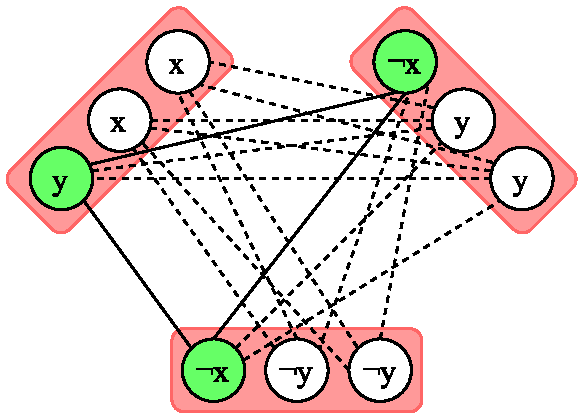
\includegraphics[width=0.5\textwidth]{Figures/clique.pdf}
\caption{Graphically showing the equivalence between 3SAT and the clique problem, implying the clique problem is NP-complete.}
\label{fig:clique}
\end{figure}

\subsubsection{Minimum Vertex Cover}

The goal of the minimum vertex cover problem is to find a subset, $V'$, of vertices of a graph such that every edge in the graph has at least one endpoint in $V'$, and such that the sum of the costs of the chosen vertices is minimised. This can be formulated as an integer linear program,

\begin{align}
\begin{array}{rl}
\text{minimise} & z = \sum_v c(v)x_v \\
\text{subject to} & x_u + x_v \geq 1, \forall \{u, v\} \in E, \\
& x_i \in \{0, 1\}
\end{array}
\label{eq:vertexcover}
\end{align}

where $c(v)$ denotes a cost function for a vertex $v$ and $x_v$ is set to one if the vertex $v$ is selected for the cover.

\subsection{Graph Traversal}

The act of traversing a graph is to visit each of its nodes exactly once, according to some ordering. Two main strategies may be used: depth-first search (DFS) and breadth-first search (BFS). A DFS visits the descendants of a node before visiting its siblings, that is, traversing sub-branch by sub-branch. A BFS visits the siblings of a node before visiting its descendants, that is, traversing depth by depth. Pseudo-code for DFS and BFS is given in Algorithms \ref{alg:dfs} and \ref{alg:bfs} respectively. When the graph has a tree structure (only branching, no converging), there is a single path to each node from the root, hence marking nodes as visited is unnecessary. Traversal may, for example, be used to exhaustively locate a particular node in the graph. A BFS has the potential advantage of facilitating a depth cutoff, searching each depth exhaustively and one at a time. However, there is then a space requirement to queue descendants in some internal memory structure, and for a ballooning tree structure such as in a chess \emph{game tree}, storing more than a few levels or \emph{ply} is infeasible.

\begin{algorithm}
\caption{Pseudocode for a depth-first search (DFS).}\label{alg:dfs}
\begin{algorithmic}[1]
\Procedure{InitDFS}{graph}
\State DFS(graph$\rightarrow$root)
\EndProcedure
\Procedure{DFS}{node}
\State node$\rightarrow$MarkAsRead()
\For {child in node$\rightarrow$children}
\If{NOT child$\rightarrow$AlreadyRead()}
\State DFS(child)
\EndIf
\EndFor
\EndProcedure
\end{algorithmic}
\end{algorithm}

\begin{algorithm}
\caption{Pseudocode for a breadth-first search (BFS).}\label{alg:bfs}
\begin{algorithmic}[1]
\Procedure{BFS}{graph}
\State queue $\leftarrow$ [ ]  \//* initialise FIFO queue *\//
\For {child in graph$\to$root$\to$children}
\State queue$\rightarrow$Enqueue(child)
\EndFor
\While {NOT queue$\rightarrow$IsEmpty()}
\For {child in queue$\rightarrow$front$\rightarrow$children}
\If{NOT child$\rightarrow$AlreadyRead()}
\State queue$\rightarrow$Enqueue(child)
\EndIf
\EndFor
\State queue$\rightarrow$Dequeue(queue$\rightarrow$front)
\EndWhile
\EndProcedure
\end{algorithmic}
\end{algorithm}

\subsection{Shortest Path Problem}

A common problem to compute over a weighted graph is the shortest path between a source node and sink node within the graph. Perhaps the two most famous shortest path algorithms are Dijkstra's algorithm and the Bellman-Ford algorithm.

\subsubsection{Dijkstra's Algorithm}

Given a weighted graph, Dijkstra's algorithm, discovered by Dutch computer scientist,  Edsger W. Dijkstra (1930-2002), finds the shortest path from a source node to all other nodes in a graph. In practice, the goal is to find the shortest path from a source node to a unique sink node, but Dijkstra's algorithm computes shortest paths to all nodes as a matter of course. The algorithm consists of visiting each node in order of closeness (initially the source node has zero distance and all others are infinite). Each neighbour of the current node is then inspected, and its shortest distances updated, if it so happens that a shorter path can reach it via the current node. After a node has been visited, it is discarded, and the algorithm terminates once all nodes have been visited. Aside from a shortest distance, nodes record the node from which its shortest path derives, such that at the end, the shortest path can be traced back from sink to source. The algorithm runs in $O(N\log N)$ time in the worst case, where $N$ is the number of vertices.

\section{Introduction to Machine Learning}

Machine learning seeks to construct algorithms that create mathematical models or \emph{machines}, predictive or descriptive, over a set of data. The field utilises an amalgamation of applied mathematics techniques from probability, linear algebra, and optimisation theory. Here we specify a glossary of important terms in machine learning.

\subsection{Learning}

In machine learning, learning refers to optimising a model to generalise over a data set. A machine learning task will follow one of the following fundamental approaches, which depend on the nature of the data $\mathcal{D}$ to be learned from:

\subsubsection{Supervised Learning}

in this case, $\mathcal{D} = \{\mathbf{X}, \mathbf{y}\}$ is \emph{labelled}, that is, each data sample, $\mathbf{x}_i$, has a corresponding output, $y_i$, which is real-valued for a regression task, and discrete for classification\footnote{Note the output may further be scalar- or vector-valued, though we will focus on scalar-valued outputs.}. The task of supervised learning is therefore to learn the mapping that best approximates $\mathbf{y}$ from $\mathbf{X}$. This is by far the most common form of machine learning, which includes many well known techniques, such as regressions, decision trees, support vector machines, and neural networks.

\subsubsection{Unsupervised Learning}

In this case $\mathcal{D} = \{\mathbf{X}\}$ is unlabelled and the learning task is to extract patterns from the data in and of itself. It is sometimes also known as \emph{knowledge discovery}. For example, we might want to find how to reasonably group the observations in $\mathcal{D}$, a task known as clustering. This is arguably the part of machine learning that is most like human learning in that rules are inferred without external confirmation. Unlike supervised learning, which sports a profusion of techniques, unsupervised learning techniques are less extensive and understood. Unsupervised learning is a sort of holy grail of machine learning.

\subsubsection{Semi-Supervised Learning}

In this case, the dataset is a mixture of both labelled and unlabelled data. In many practical problems, labelled data is hard to come by, but unlabelled data might be abundant. Semi-supervised techniques seek to combine the data in a reliable way. This approach to learning has shown surprisingly limited success so far.

\subsubsection{Transfer Learning}

Transfer learning (\cite{transfersurvey}) refers to a broad variety of techniques that use the solution of one problem in solving another. Arguably, supervised machine learning is subsumed by the transfer learning framework, but where the source and target domains are the same, and where training is performed as a single step.

\subsubsection{Deep Learning}

Deep learning refers to approaches that aim to model a hierarchy of abstractions in a dataset. One famous example are deep convolutional neural networks form computer vision, which ``stack'' multiple convolutional hidden layers in sequence, each layer modeling finer features of its input images. These models have shown tremendous success in computer vision tasks in recent years, making vast improvements on the earlier state of the art. Another example are deep belief networks, which are restricted Boltzmann machines (RBM)\footnote{RBMs are a generative neural networks factorising over a bipartite graph (hence, \emph{restricited}). Similarly to autoencoders, they can be used in an unsupervised fashion to learn a feature representation in terms of \emph{latent variables}.} stacked one after the other.

%\subsection{Learning Schemes}
%
%The following schemes refer to how the data is \text{used}, rather than the nature of the data (as above):
%
%\subsubsection{Reinforcement learning}
%In this case, learning incorporates occasional feedback signals in a trial and error framework.
%
%\subsubsection{Active learning}
%Refers to a scheme whereby training data can be actively selected.
%
%\subsubsection{Online learning}
%Refers to where models are trained on data samples that arrive one by one rather than all at once, as if streamed.
%
%\subsubsection{Ensemble learning}
%Ensemble models train multiple `weak' models on subsets of the data, then aggregate their individual predictions. Random forests are an example of this, where many decorrelated decision trees are trained in an effort to reduce variance. Adaboost (adaptive boosting) is a famous boosting  meta-algorithm.

\subsection{Training and Prediction}

Here we define some key concepts surrounding the training and prediction of models.

\subsubsection{Feature Engineering} Feature engineering is the exercise of designing features, according to some ontology about the model. This is an opportunity for domain knowledge to be imparted into a model, with the view of making more indicative features. This is an inherently soft science, but constitutes a large part of applied machine learning in practice. \emph{Feature extraction} is a separate concept, which, for example, may use unsupervised learning to derive features for modelling.

\subsubsection{Training} Training or learning is the act of inferring model parameters from a dataset through some sort of optimisation algorithm. It is vitally important to (randomly) set aside some data from the start, because there must be some independent data available to validate the trained model. If we use all data on training, it is impossible to know how it will perform on unseen data. The usual scheme is to first split the data into training and test datasets. The test data is strictly separated from the training process. A part of the training set is extracted as a validation set. These split sizes follow some loose convention, leaving the majority of data for training, for example a $50-25-25$ split. Models are trained on a training set and its predictive performance is assessed on a validation set, providing a benchmark to compare choices of model and model hyper-parameters. This is a process known as \emph{model selection} (\cite{htf}).

\subsubsection{Cross-Validation}
When data is scarce, we can simulate having a validation set in a procedure called cross-validation (CV). Cross-validation partitions the training data into $K$ validation \emph{folds}. A model is trained on the first $K - 1$ folds, and validated on the final fold. This process is repeated $K$ times, such that each fold is validated on, giving $K$ samples for estimating error. If the fold size is chosen to be a single sample (that is, $K = N$), we have leave-one-out cross-validation (LOOCV). The chosen model will be the one that minimises the average CV error. A model is then trained on all the training data (including validation data), and the resulting model tested on the test data. The predictions made are compared with the true values, giving an estimation of generalisation error that can then be reported, in a process known as \emph{model assessment}.

\subsubsection{Generalisation Error}
Generalisation error refers to the expected test error averaged over all possible datasets. As such complete coverage of data is in practice never available, an estimate can be found using cross-validation. As more data is added, the predictive power (generalisation error) of the model improves, as the approximation error (the discrepancy between the estimate and the best estimate given the choice of model) in the model parameters is minimised.

\begin{figure}
\centering
\begin{tabular}{cc}
\subfloat[$k = 1$]{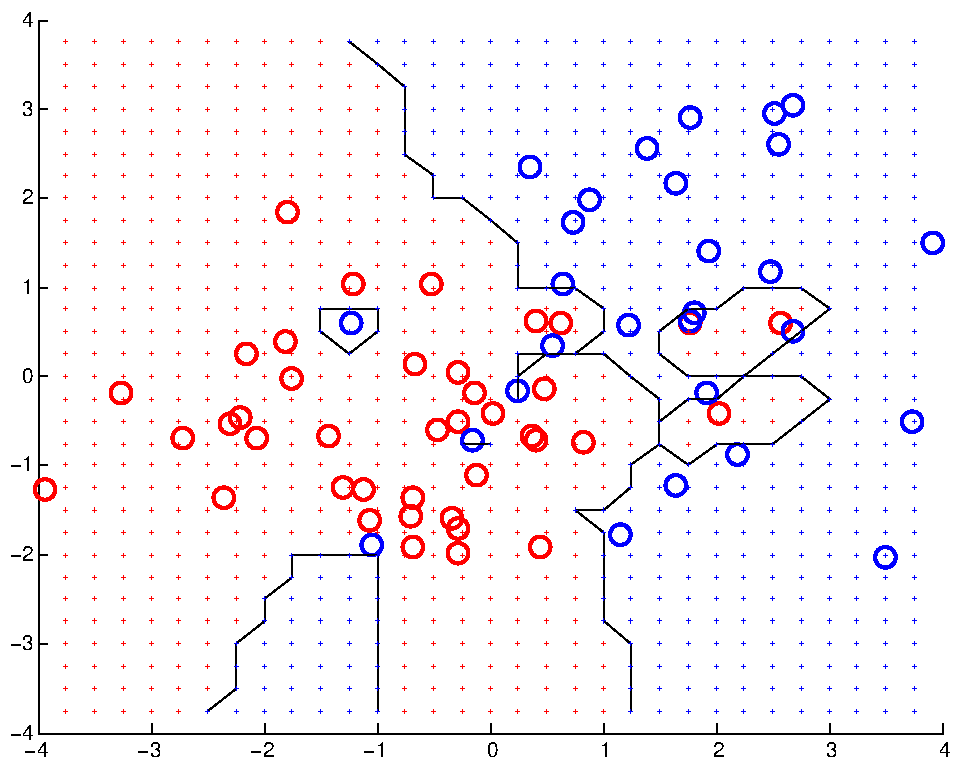
\includegraphics[width=0.5\textwidth]{Figures/knn1.pdf}} & 
\subfloat[$k = 7$]{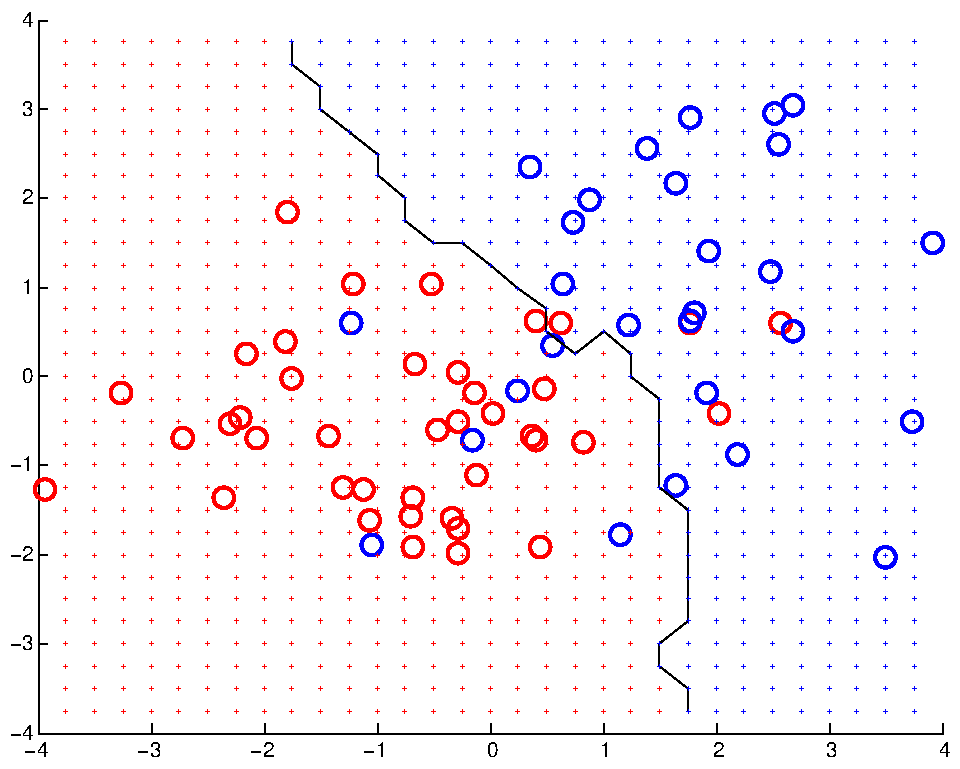
\includegraphics[width=0.5\textwidth]{Figures/knn7.pdf}}
\end{tabular}
\caption{Visualisation of overfitting with k-nearest neighbours (kNN) (non-parametric model). A data point is classified as the majority class of the $k$ geometrically closest data points. Note the steadier decision boundary formed for $k = 7$. This classifier can be very effective, but suffers from the curse of dimensionality. Data normalisation and dimensionality reduction usually help. However, in certain high-dimensional data sets where data is confined to a lower-dimensional manifold, for example in OCR data, kNN can be very effective. Unlike most classifiers, test time is much greater than training time. Approximations using memory tradeoffs mitigate this. Created with \texttt{knnDemo.m}.}
\label{fig:knn}
\end{figure}

\subsubsection{Overfitting} Overfitting is a constant danger when training models. This is the effect of \emph{fitting the noise instead of the signal}. All data contains noise, and when the dataset is sufficiently small and the model sufficiently complex (e.g. a high degree polynomial), the model can fit the training data perfectly, only to be useless on test data. Take for example a k-nearest neighbours (kNN) classifier (Figure \ref{fig:knn}). For small $k$, outliers have unreasonable influence on local test data, creating discontinuous decision boundaries. There are various strategies to attenuate overfitting. The most ideal is to increase the amount of data available for training, but this is rarely an option. A more typical approach is \emph{regularisation}. This usually takes the form of a penalty term, but really corresponds to imposing a prior distribution on the parameter set. A prior distribution assigns low probabilities to large parameter values. Complex models that overfit usually require large parameter values to make a fit, so regularisation curtails this tendency. Another, more drastic approach, is to change the form of the cost function (likelihood) of the model to insulate it from outliers in the data. An example of this is robust regression, where a Laplace likelihood replaces a Gaussian. A variant of overfitting is the zero count (sparse data) problem, where specific data that ought to be modelled has not appeared in the dataset and leads to a zero probability prediction. \emph{Underfitting} occurs when the complexity of the model is insufficient to capture the trends of the data. This can be addressed by modifying the choice of basis function or kernel, otherwise by choosing a different technique.

\subsubsection{Ground Truth}
Ground truth is a somewhat nebulous term usually referring to a supervised data set, in particular, that which can be assumed to be correct, and which is to be assimilated by a model. It differs from those patterns that are inferred, for example in an unsupervised setting. The term comes from the field of earth sciences where it refers to data measured directly on the ground, or in the atmosphere, rather than indirect data samples collected from, for example, satellite imagery. The \emph{gold standard} is a related term from statistics that refers to the convention for the best possible statistical test one can perform. What qualifies as the gold standard varies according to the context. In practice, it is shorthand for indicating that a statistical study conforms to the highest possible standard.

\subsubsection{The Curse of Dimensionality}
The curse of dimensionality refers to the difficulty of generalising over a small amount of high-dimensional data. This is because the observation state space grows exponentially as features are added. We therefore need to increase our data exponentially to maintain good coverage. Automatic techniques such as principal components analysis (PCA) exist for \emph{dimensionality reduction} of data, in which the data is mapped to a lower-dimensional space representing the axes of highest variance (trends) of the data. Another option is to encourage model sparsity using $l_1$ regularisation. This tends to build models that ignore unimportant features. Various 
feature selection techniques also exist, where an optimised subset of features is selected according to preprocessing (filtering), cross-validation (wrapping), or as part of the learning algorithm itself (embedding) (\cite{transfersurvey}).

\subsubsection{Bias-Variance Decomposition}
The bias-variance tradeoff refers to a result illustrating the expected behaviour of a parameter estimate, with respect to the `true' parameters it approximates. Bias represents \emph{underfitting}, and variance represents \emph{overfitting}. Underfitting/bias is observed in training error; overfitting/variance in test error. This tradeoff is reflected in the \emph{no free lunch theorems}\footnote{No free lunch in machine learning refers to the fact that, averaged over all possible ground truths, no model is better than random guessing. This illustrates the power of the implicit assumptions we make when modelling data, for example, that the ground truth function is smooth with Gaussian noise. It  If the data is uniformly random, there will be` no signal to learn.}.

 Let $Y = f(x) + \epsilon$ be the ground truth value with $f(x)$ the true signal for data point $x$, and noise, $\epsilon = \mathcal{N}(0, \sigma^2)$. Let our model estimate be denoted by $\hat{f}(x)$. Then, the MSE between an estimate and the true parameters, averaged over all possible data,

\begin{align}
\mathbb{E}[(Y - \hat{f}(x))^2] &= \mathbb{E}[((f(x) + \epsilon - \mathbb{E}[\hat{f}(x)]) + (\mathbb{E}[\hat{f}(x)] - \hat{f}(x)))^2] \notag \\
&= \sigma^2 + \mathbb{E}[f(x) - \mathbb{E}[\hat{f}(x)]]^2 + \mathbb{E}[(\hat{f}(x) - \mathbb{E}[\hat{f}(x)])^2] \notag \\
&= \text{noise} + \text{bias}^2 + \text{variance} \notag
\end{align}

The discrepancy therefore depends both on the variance of the parameters around its own mean, and the bias (the gap between this estimate mean and the true parameters\footnote{The flaw here is that we require the structural assumptions of the model to be correct before we can talk about `true' parameters, which is rarely the case. This discrepancy is known as `structural error'. Even if the model structure is correct, there is an inescapable error of noise that all models share called the \emph{noise floor}. The noise floor is the limit of the learning curve (the trend of improvement in generalisation error as data is added) for an unbiased estimate.}). An unbiased estimate is a parameter model (for example MLE) that converges (in probability) to a hypothetical true parameter set as data increases, but it may entail a higher variance, making it more likely to draw a bad estimate some of the time. Hence, if we wish to be more certain about the optimality of our estimate, it may be prudent to allow some bias (for example through regularisation) if it sufficiently reduces the variance. In conclusion, the bias-variance tradeoff illustrates that on average it may benefit to use a ridge regression rather than OLS regression, even though this invokes a small bias.

\subsubsection{Gauss-Markov Theorem}

Orthogonal to the bias-variance tradeoff is the Gauss-Markov theorem. This shows that among unbiased linear models, the one with lowest variance is ordinary least squares. This is thus a statement on the choice of loss function, in contrast to bias-variance, which is a statement about regularisation. In effect, it is a fundamental result, though somewhat tautological: ``the best way to minimise variance is to infer parameters that minimise mean square error, that is, variance''.

\section{Bayes and the Beta-Binomial Model}

We begin by examining the primordial Beta-Binomial model--that which was studied by English mathematician, Thomas Bayes (1701-1761), in \emph{An Essay towards solving a Problem in the Doctrine of Chances}\footnote{This early term for probability theory comes from de Moivre's seminal textbook (1718).}. Here we consider inference over data produced from a sequence of coin tosses, such as, $$0101001010111,$$ where $0$ represents `tails' and 1 `heads'. In fact, it is sufficient to know the number of heads and tails, which we denote $N_1$ and $N_0$ respectively. These are known as `sufficient statistics'. Note that the beta-binomial model is not a classifier, as we are not engaging in \emph{classification}, but rather we are predicting a single next outcome. The starting point is to define the likelihood. The probability distribution for such a random sequence is the discrete binomial distribution. As we are maximising for the rate parameter, we can drop the normalisation constant and we have,

$$p(\mathcal{D}|\theta) = \theta^{N_1}\cdot(1 - \theta)^{N_0}.$$

Clearly, we can maximise this expression by taking the derivative to give,

\begin{align}
N_1\theta^{N_1 - 1}(1 - \theta)^{N_0} - N_0\theta^{N_1}(1 - \theta)^{N_0 - 1} &= 0 \notag \\
&\implies \hat\theta_{MLE} = \frac{N_1}{N_0 + N_1} = \frac{N_1}{N}, \notag
\end{align}

where $N = N_0 + N_1$. The prior distribution is chosen to be \emph{conjugate} to the likelihood, that is, of like form. The continuous beta distribution is therefore a suitable choice, hence,

$$p(\theta) = \text{Beta}(\theta|a, b) \propto \theta^{a - 1}(1 - \theta)^{b - 1},$$ where we drop the normalising beta function for the proportionality. The values of $a$ and $b$ are hyper-parameters that control the skew. When $a = b = 1$, we have a uniform prior and the posterior is just the same as the likelihood. We multiply the prior and likelihood to obtain the posterior,

$$p(\theta|\mathcal{D}) \propto \theta^{N_1 + a}\cdot(1 - \theta)^{N_0 + b}.$$

Notice how the hyper-parameters behave as additional observations. For this reason they are known as \emph{pseudo-counts}--it is as though we had some additional data other than $\mathcal{D}$ that we can use to influence or stabilise the behaviour of the posterior. This is the power of a prior distribution. Now, the beta distribution distributes the continuous $\theta$, so this time we can simply look up the mode of a beta distribution to obtain the MAP estimate,

$$\hat\theta_{MAP} = \frac{N_1 + a - 1}{N + a + b - 2}.$$ Notice that as $N \to \infty$, the MAP estimate approaches the ML estimate. This shows that a prior serves its role of stabiliser only for smaller data sets. As data is added, it is overwhelmed by the volume of data fitted by the likelihood. Now, the posterior predictive distribution for unseen data, $\hat{x}$, is either given directly by the ML or MAP estimates, or else from Bayes model averaging,

\begin{align}
p(\hat{x} = 1|\mathcal{D}) &= \int_0^1 p(x = 1 |\theta)p(\theta|\mathcal{D})\mathop{dx} \notag \\
&= \int_0^1 \theta p(\theta|\mathcal{D})\mathop{dx} = \mathbb{E}[\theta|\mathcal{D}] = \frac{N_0 + a}{N + a + b}. \notag
\end{align}

The mean of a beta distribution differs from its mode, as it is asymmetric.

\section{Generative Classifiers}

Here we describe \emph{generative classifiers}, by illustrating how their components are derived with the naive Bayes classifier (NBC). A classifier is simply a model that predicts the membership of an observation, $x$, in one of a discrete number of classes. Generative classifiers `generate' the posterior distribution through inference, in contrast to \emph{discriminative} classifiers, which model the posterior distribution directly. The parameters of a NBC are found by considering the likelihood for $N$ data training samples, $\mathcal{D}$, of dimension $D$, which may be written,

\begin{align}
\textbf{likelihood} = p(\mathcal{D}|\theta) = p(\mathbf{X}, \mathbf{y}|\boldsymbol\theta) &= p(\mathbf{y}|\boldsymbol\theta)p(\mathbf{X}|\mathbf{y},\boldsymbol\theta) \notag \\
&= \textbf{class prior} \times \textbf{class conditional density} \notag \\
&= \prod_{i=1}^N p(y_i|\boldsymbol\pi)p(\mathbf{x}_i|y_i,\boldsymbol\theta), \label{eq:iid} \\
&= \prod_{i=1}^N p(y_i|\boldsymbol\pi)\prod_{j = 1}^D p(x_{ij}|y_i,\boldsymbol\theta_j), \label{eq:nbc}
\end{align}

where we denote the set of parameters for both input and output variables, $\boldsymbol\theta = \{\boldsymbol\pi, \boldsymbol\theta\}$. Step (\ref{eq:iid}) follows from the data being independent and identically distributed (a standard assumption), and step (\ref{eq:nbc}) from the naive Bayes assumption of feature independence when the class is given\footnote{This is called a naive assumption because it precludes covariance between model features, which in practice is usually present.} We take logarithms to derive the log-likelihood, a common trick that makes optimisation easier without changing the optimal parameters,

\begin{align}
\log p(\mathcal{D}|\boldsymbol\theta) &= \sum_{i=1}^N \log p(y_i|\boldsymbol\pi) + \sum_{i=1}^N\sum_{j = 1}^D\log p(x_{ij}|y,\boldsymbol\theta_j) \notag \\
&= \sum_{c} N_c\log \boldsymbol\pi_c + \sum_{c}\sum_{i:y_i=c}\sum_{j = 1}^D\log p(x_{ij}|y=c,\boldsymbol\theta_{jc}), \notag
\end{align}

where $N_c$ is the number of observations having class $c$. Now we have an expression that is easy to optimise, we can obtain the \textbf{maximum likelihood estimate} (MLE) by optimising each of the parts of the sum. This is equivalent to calculating the \emph{mode} of each of the probability functions. For the multinomial class variable, the task is simple, $\hat\pi_c = N_c/N.$ For the input parameters, the MLE depends upon the choice of distribution. One of the benefits of the naive independence assumption is it allows us to model any combination of distributions with ease--all we need do is substitute their probability functions. For illustration, we may simply opt for Bernoulli distributions on each of the features. Hence, the mean for feature $j$ given class $c$ is $\hat\theta_{jc} = N_{jc}/N_c$, where $N_{jc} = \sum_{i:y_i=c} x_{ij}$, noting the $x_{ij}$ are binary. The maximum likelihood estimate is therefore, $\hat{\boldsymbol\theta}_{MLE} = \{\hat\pi_c, \hat\theta_{jc} : 1\leq c\leq C, 1\leq j\leq D\}$. This is now enough to make a prediction. The posterior predictive distribution derives from,

\begin{align}
\textbf{posterior predictive} = p(y = c|\mathbf{x},\boldsymbol\theta) 
&= \frac{p(y = c|\boldsymbol\theta)p(\mathbf{x}|y=c,\boldsymbol\theta)}{\sum_{c'}p(y = c'|\boldsymbol\theta)p(\mathbf{x}|y=c',\boldsymbol\theta)} \notag \\
&\propto p(y = c|\boldsymbol\theta)p(\mathbf{x}|y=c,\boldsymbol\theta), \label{eq:postpred}
\end{align}

having the same form as (\ref{eq:nbc}). For a test observation, $\hat{\mathbf{x}}$, we can simply cycle through each of the classes, plug the appropriate parameters into (\ref{eq:postpred}), and compute a probability. We can then predict the classification of $\mathbf{x}$ to be the class $c$ having maximum probability. This is called a \textbf{plug-in approximation}, and it is the first of two alternatives for prediction. We will come to the other shortly, but first there are several more things we can do with plug-in approximation. To begin with, we may wish to include \emph{prior} information on the parameters. Thus, we form the prior distribution,

\begin{align}
\textbf{prior} = p(\boldsymbol\theta) = p(\boldsymbol\pi)\prod_c\prod_{j=1}^Dp(\theta_{jc}). \notag
\end{align}

The prior imposes a distribution on the parameter set, which has a stabilising effect when the training data is limited, mitigating overfitting. We choose the prior distributions on the parameters to be \emph{conjugate} to the likelihood distributions, that is, having a similar form. This is by no means compulsory, but it makes the derivations easier. Since we have a multinomial distribution on $y$ and Bernoulli distributions on $x|y=c$, we choose Dirichlet and beta distributions respectively for the prior parameters. Thus, $\boldsymbol\pi \sim \text{Dir}(\boldsymbol\alpha)$ and $\boldsymbol\theta_j \sim \text{Beta}(\beta_0, \beta_1)$. Choosing $\boldsymbol\alpha = \mathbf{1}$ and $\boldsymbol\beta = \mathbf{1}$ corresponds to a common practice known as \emph{add one} smoothing.

If we combine the prior with the likelihood, we get the posterior distribution, which strikes a balance between what the data tells us and what we expect in advance,

\begin{align}
\textbf{posterior} = p(\boldsymbol\theta|\mathcal{D}) &\propto \textbf{likelihood} \times \textbf{prior} \notag \\
&= \prod_{n=1}^N\text{Cat}(y_i|\boldsymbol\pi)\text{Dir}(\boldsymbol\pi;\boldsymbol\alpha)\prod_{c}\prod_{i:y_i = c}\prod_{j = 1}^D \text{Ber}(x_{ij}|\theta_{jc})\text{Beta}(\theta_{jc};\beta_0, \beta_1), \notag \\
&= p(\boldsymbol\pi|\mathcal{D})\prod_{j = 1}^D p(\boldsymbol\theta_{j}|\mathcal{D}), \notag
\end{align}

where $p(\boldsymbol\pi|\mathcal{D}) = \text{Dir}(N_1 + \alpha_1, \dots, N_C + \alpha_C)$ is the posterior on $\boldsymbol\pi$, and $p(\boldsymbol\theta_{j}|\mathcal{D}) = \text{Beta}((N_c - N_{jc}) + \beta_0, N_{jc} + \beta_1)$ is the posterior on $\boldsymbol\theta_{j}$. Note that because we are optimising for $\boldsymbol\theta$, it does not matter that the expression is only proportional to the posterior. Also note that if we have a uniform prior, the probabilities are constant, and the posterior is equivalent to the likelihood. Now we have two options: firstly, we can compute the mode of this posterior distribution giving us the \textbf{maximum a posteriori estimate}, $\hat{\boldsymbol\theta}_{MAP}$. This can then be plugged into the posterior predictive, just as with the MLE. The alternative is to use \textbf{Bayes model averaging}. This calculates the posterior as a weighted average of the distribution. In this scheme, neither the ML or MAP estimates are computed directly, rather, we sum or integrate over the unknown parameters, marginalising them,

\begin{align}
p(y = c|\hat{\mathbf{x}}, \mathcal{D}) &= \frac{p(\hat{\mathbf{x}}|y = c, \mathcal{D})p(y=c|\mathcal{D})}{\sum_{c'}p(\hat{\mathbf{x}}|y = c', \mathcal{D})p(y=c'|\mathcal{D})} \notag \\ &\propto p(\hat{\mathbf{x}}|y = c, \mathcal{D})p(y=c|\mathcal{D}) \notag \\
&= \int p(\hat{\mathbf{x}}, \boldsymbol\theta|y = c, \mathcal{D})\mathop{d\boldsymbol\theta}\int p(y=c, \boldsymbol\pi|\mathcal{D})\mathop{d\boldsymbol\pi} \label{eq:ltp} \\
&= \int p(\hat{\mathbf{x}}|y = c, \boldsymbol\theta, \cancelto{}{\mathcal{D}})p(\boldsymbol\theta|\cancelto{}{y = c}, \mathcal{D})\mathop{d\boldsymbol\theta}\int p(y=c|\boldsymbol\pi, \cancelto{}{\mathcal{D}})p(\boldsymbol\pi|\cancelto{}{y = c}, \mathcal{D})\mathop{d\boldsymbol\pi}, \label{eq:cancel}
\end{align}

where step (\ref{eq:ltp}) comes form the law of total probability and the cancellations in step (\ref{eq:cancel}) occur because the prediction is independent of the data when conditioned on the parameters. Thus we are averaging by the posterior distribution. This may be solved analytically for the choice of distributions we have made. Now, a retrospective connection to plug-in approximation may be seen. Plug-in approximation works on the assumption that the distribution on the parameters, $p(\theta|\mathcal{D}) \to \delta_{\hat{\theta}_{MAP}}(\theta)$ as $|\mathcal{D}| \to \infty$. This follows the intuition that increasing data increases our certainty about the parameters. If we replace the posteriors in the integral with the limit, then by the sifting property of the Dirac delta function, we obtain the class conditional and class prior distributions, conditioned on the MAP estimate--the plug-in approximation. A simple implementation of the naive Bayes classifier is given in \texttt{nbcDemo.m}. 

\section{Multivariate Normal Distribution}
The multivariate Normal (MVN) or multivariate Gaussian distribution is the multidimensional generalisation of the univariate Gaussian distribution. The form of the probability density function for a $D$-dimensional Gaussian is defined to be,

$$\mathcal{N}(\mathbf{x} ; \mu, \Sigma) \triangleq \frac{1}{(2\pi)^{D/2}|\boldsymbol\Sigma|^{1/2}}
\exp\bigg[-\frac{1}{2}(\mathbf{x} - \boldsymbol\mu)^T\boldsymbol\Sigma^{-1}(\mathbf{x} - \boldsymbol\mu)\bigg]
$$

where the vector $\boldsymbol\mu$ is the vector of means and $\boldsymbol\Sigma$ is the covariance matrix. The exponent expresses the Mahalanobis distance (named after Indian statistician Prasanta Chandra Mahalanobis (1893-1972)), which captures the behaviour of mean squared error in $D$ dimensions. The covariance matrix is by definition symmetric positive semi-definite, and may be diagonalised with a diagonal matrix of eigenvalues, $\boldsymbol\Lambda$, and orthonormal eigenvectors, $\mathbf{U}$, as $\boldsymbol\Sigma = \mathbf{U}\Lambda\mathbf{U}^T$ where orthonormality implies $\mathbf{U}^{-1} = \mathbf{U}^T$. Consequently,

$$\boldsymbol\Sigma^{-1} = \mathbf{U}^T\Lambda^{-1}\mathbf{U} = \sum_{d=1}^D\frac{1}{\lambda_d}\mathbf{u}_d\mathbf{u}_d^T,$$

where $\mathbf{u}_d$ are the columns of $\mathbf{U}$. Therefore, the Mahalanobis distance can be expressed as,

$$(\mathbf{x} - \boldsymbol\mu)^T\Sigma^{-1}(\mathbf{x} - \boldsymbol\mu) = \sum_{d=1}^D\frac{y_d^2}{\lambda_d^2},$$

where $y_i = \mathbf{u}_i^T(\mathbf{x} - \boldsymbol\mu)$, from which it may be seen that events of equal probability lie along elliptical contours, for which the eigenvectors form the axes and eigenvalues control the distortion. Fitting a MVN from data $\mathcal{D}$ of size $N$ can be done with maximum log-likelihood estimation. With a bit of vector calculus, the MLE is,

$$\hat{\boldsymbol\mu}_{MLE} = \frac{1}{N}\sum_{n=1}^N\mathbf{x}_n,$$

that is, the sample mean and,

$$\hat{\boldsymbol\Sigma}_{MLE} = \frac{1}{N}\sum_{n=1}^N(\mathbf{x}_i - \boldsymbol\mu)(\mathbf{x}_i - \boldsymbol\mu)^T,$$

the sample covariance matrix.

\subsection{Gaussian Discriminant Analysis}

Gaussian discriminant analysis is a family of classifiers that fit Gaussian distributions to each of $K$ classes. That is, the class-conditional densities are defined to be,

$$p(\mathbf{x} | y = c) = \mathcal{N}(\mathbf{x} ; \hat{\mu}_c, \hat\Sigma_c),$$

where the parameters come from the maximum likelihood for multivariate normal distributions (MVN). Where the covariance matrix is diagonal, the features are independent, and this is equivalent to the naive Bayes classifier. This sort of modelling, where we learn $K$ Gaussian densities and predict membership of a test observation is effectively a generalisation of a nearest centroids classifier\footnote{A nearest centroids classifier is one of the simplest classifiers imaginable. Training is performed by computing centroids for points in each class of training data, $\boldsymbol\mu_c = 1/|c|\sum_{i:y_i=c}\mathbf{x}_i$. A prediction for unseen data $\hat{\mathbf{x}}$ is then made as $\hat{y} = \min_c ||\hat{\mathbf{x}} - \boldsymbol\mu_c||$, that is, the class of the nearest centroid.}.

\subsubsection{Quadratic Discriminant Analysis}

The posterior predictive distribution can then be defined as,

$$p(y = c|\mathbf{x}, \theta) = \frac{\pi_c(2\pi)^{-D/2}|\boldsymbol\Sigma|^{-1/2}\exp\big[-\frac{1}{2}(\mathbf{x} - \mathbf{\mu}_c)^T\boldsymbol\Sigma_c^{-1}(\mathbf{x} - \boldsymbol\mu_c)\big]}{\sum_{c'}\pi_{c'}(2\pi)^{-D/2}|\boldsymbol\Sigma|^{-1/2}\exp\big[-\frac{1}{2}(\mathbf{x} - \boldsymbol\mu_{c'})^T\boldsymbol\Sigma_{c'}^{-1}(\mathbf{x} - \boldsymbol\mu_{c'})\big]},$$

where $\pi_c$ is the class prior. It may be shown (though we will not do so here) that a decision rule\footnote{A decision rule is a probability threshold for classification, usually equal to 0.5 in binary classification.} creates a quadratic boundary between the centroids in Euclidean space. Notice finally that we are effectively doing a plug-in approximation, in the absence of Bayes model averaging.

\subsubsection{Linear Discriminant Analysis}

Linear discriminant analysis (LDA) arises from QDA when the simplifying assumption is made that the covariance matrices are all equal. In this instance we have,

$$p(y = c|\mathbf{x}, \theta) \propto \exp\Big[\boldsymbol\mu_c^T\Sigma^{-1}\mathbf{x} - \frac{1}{2}\boldsymbol\mu_c^T\boldsymbol\Sigma^{-1}\boldsymbol\mu_c + \log\pi_c\Big]\exp\Big[-\frac{1}{2}\mathbf{x}^T\boldsymbol\Sigma^{-1}\mathbf{x}\Big],$$

and the quadratic term cancels out over the sum, leaving an expression that is linear in $\mathbf{x}$. It can be shown easily that this produces linear decision boundaries. There are some interesting connections between LDA and other parts of machine learning. If we define $\gamma_c = - \frac{1}{2}\mu_c^T\Sigma^{-1}\mu_c + \log\pi_c$ and $\beta_c = \Sigma^{-1}\mu_c$, we can write,

$$p(y = c|\mathbf{x}, \theta) = \frac{e^{\beta_c^T\mathbf{x} + \gamma_c}}{\sum_{c'}e^{\beta_{c'}^T\mathbf{x} + \gamma_{c'}}} = \mathcal{S}({\eta})_c,$$

where $\eta_c = [\beta_1^T\mathbf{x} + \gamma_1, \beta_2^T\mathbf{x} \gamma_2 , \dots, \beta_C^T\mathbf{x} + \gamma_C]$, and $\mathcal{S}$ is the \emph{softmax} function\footnote{The softmax function is so called because at low `temperatures', that is, if we divide all the exponents by $T$, the probability of the most likely class goes to $1$ as $T \to 0$. This terminology comes from statistical physics--in fact the softmax function has the same form as the Boltzmann distribution (Ludwig Boltzmann (1844-1906) was a German physicist credited with the development of statistical mechanics).}. The marginal likelihood is known as the partition function, denoted $Z$ for `Zustandssumme'--the German expression for `sum over states'. This form of LDA is very similar to logistic regression, differing only in the fact that LDA is generative and logistic regression is discriminative. If we normalise a naive Bayes classifier with Gaussian features, it is equivalent to LDA--hence naive Bayes and logistic regression form what is known as a generative-discriminative pair.

\section{Linear Regression}

A linear regression is used to make predictions for a continuous variable.

\subsection{Constructing a Loss Function}
The starting point for building a regression model is a dataset, $\mathcal{D}$, where,

$$\mathcal{D} = \{(\mathbf{x}_n, y_n)\}_{n=1}^{N},$$

that is, a set of $N$ data points, where $\mathbf{x}_i \in \mathbb{R}^D$ is a $D$-dimensional \emph{input} vector, and $y_i \in \mathbb{R}$ are the corresponding scalar outputs. The dataset, $\mathcal{D}$, is known as our \emph{training set}. The objective of the regression algorithm is to infer the linear function that best fits the data. More precisely, we want to find the vector of coefficients, $\boldsymbol\beta = [\beta_1, \beta_2, \dots, \beta_D]$, that gives the best approximation for,

\begin{align}
y_n &\approx \beta_1x_{n1} + \beta_2x_{n2} + \cdots + \beta_Dx_{nD} \notag \\
&= \mathbf{x}_n^T\boldsymbol\beta, \notag
\end{align}

for all $n = 1, \dots, N$. Each of the $D$ dimensions of $\mathbf{x_n}$ is known as an indicator. The greater the corresponding coefficient in the parameter vector, $\boldsymbol\beta$, the more weight this dimension has in determining the output, $y_n$. We can formulate the above as an optimisation problem,

$$\min_{\boldsymbol\beta}\mathcal{L}(\boldsymbol\beta) = \frac{1}{2N}(\mathbf{y} - \mathbf{X}\boldsymbol\beta)^T(\mathbf{y} - \mathbf{X}\boldsymbol\beta) = \frac{1}{2N}\sum_{n=1}^{N}(y_n - \mathbf{x_n}^T\boldsymbol\beta)^2,$$

where $\mathcal{L}(\boldsymbol\beta)$ is the `loss' function, expressing a \emph{mean square error} (MSE) for choosing parameter vector $\boldsymbol\beta$, that is, the average squared distance of the approximation from the true value. Note the similarity to the variance statistic. It is the job of the learning algorithm to minimise this function. It is also typical to write $\text{MSE} = \text{RSS}/N$, where RSS stands for \emph{residual sum of squares}, the non-weighted sum. Note we could have chosen any sort of loss function, but our reasons for choosing mean squared error will be revealed in the following section.

\subsection{Method of Least Squares}

The method of least squares (MLS) is a closed-form solution to a linear regression. As previously stated, it was first published in the same paper by Gauss that also first formalised the Normal distribution. We will discover the link in the following section. Using the chain rule, we may write the derivative of the loss function,

$$\frac{\delta\mathcal{L}}{\delta\boldsymbol\beta} = -\frac{1}{N}X^T(\mathbf{y} - X\boldsymbol\beta),$$

where $\mathbf{X} \in \mathbb{R}^{N\times D}$ is the matrix whose $i$th row is the $i$th $D$-dimensional vector, $\mathbf{x}_i$, and $\mathbf{y} \in \mathbb{R}^D$ is the vector whose $i$th element is the $i$th scalar, $y_i$. We can therefore minimise $\mathcal{L}(\boldsymbol\beta)$ by setting its derivative to 0, giving the normal equation,

$$\mathbf{X}^T(\mathbf{X}\boldsymbol\beta - \mathbf{y}) = 0,$$

and finally, the optimal parameter vector,

$$\boldsymbol\beta^* = (\mathbf{X}^T\mathbf{X})^{-1}\mathbf{X}^T\mathbf{y}.$$

MLS also has a nice geometric interpretation. According to the normal equation, the error, $\mathbf{X}\boldsymbol\beta - \mathbf{y}$, is minimised when it is perpendicular to the hyperplane defined by $\mathbf{X}^T$. That is,

\begin{align}
\mathbf{X}^T\mathbf{e} &= \mathbf{0} \notag \\
\implies \mathbf{e}^T\mathbf{X}\mathbf{a} &= 0, \forall \mathbf{a}, \notag
\end{align}

where $\mathbf{e} = \mathbf{X}\boldsymbol\beta - \mathbf{y}$ is the error vector. Thus, the optimal parameters occur when the error is orthogonal to all vectors in the span of $\mathbf{X}$, that is, when it is normal to the plane. This makes intuitive sense, because it means the choice of prediction, $\mathbf{X}\boldsymbol\beta$, that minimises the distance to the true value, $y$, is the one directly `below' it on the hyperplane, $\mathbf{X}^T$. This solution is known as the ordinary least squares (OLS) solution.

\subsection{The Gram Matrix}

For the closed-form method of least squares, we require the \emph{gram} matrix $\mathbf{X}^T\mathbf{X}$ to be invertible. If $\mathbf{X}$ is full rank then $\mathbf{X}\mathbf{a} = \mathbf{0}$ iff $\mathbf{a} = \mathbf{0}$\footnote{A matrix is full rank if its columns are linearly independent. By the rank-nullity theorem, full rank implies a zero-dimensional null space or kernel.}. Therefore, $\mathbf{a}^T\mathbf{X}^T\mathbf{X}\mathbf{a} \geq 0$, implying the gram matrix is positive-definite, and therefore invertible. Note that when $N < D$ and we have a `fat' $\mathbf{X}$, $\mathbf{X}$ is often rank deficient. Even when the gram matrix is invertible, it may still be ill-conditioned. This arises when a high degree of \emph{multicolinearity} is present in the data. This refers to high degrees of correlation between features. Ill-conditioning is a concept common in numerical analysis, and in linear algebra it is captured by the \emph{condition number} of a matrix. This provides an upper bound on the relative error between solutions for changes in the data. A high condition number indicates parameters may vary significantly for small changes in the data. This can lead to problems in practice, when floating point arithmetic introduces small inaccuracies. It can be shown that the condition number, $\kappa({\mathbf{A}}) = ||\mathbf{A}||\cdot||\mathbf{A}^{-1}|| = \boldsymbol\sigma_{max}/\boldsymbol\sigma_{min}$, that is, the ratio of the largest and smallest eigenvalues of $\mathbf{A}$. Geometrically, this makes sense. Consider the way a matrix transforms a unit circle of vectors in two dimensions. When one eigenvalue dominates the other, vectors are mostly `stretched' in the direction of the first eigenvector. We would find that a small change in the direction of the second eigenvector corresponds to a much larger change in the direction of the first. `Lifting' the eigenvalues (thereby reducing the condition number) is a convenient outcome of ridge regression. This is easily seen by considering the \emph{orthonormal}\footnote{Note it is always possible to make an eigendecomposition orthonormal by dividing the eigenvectors by their norms and scaling the eigenvalues accordingly.} eigendecomposition of the gram matrix, then $\mathbf{X}^T\mathbf{X} + \lambda\mathbf{I} = \mathbf{U}\boldsymbol\Sigma\mathbf{U}^T + \lambda\mathbf{I} = \mathbf{U}(\boldsymbol\Sigma + \lambda\mathbf{I})\mathbf{U}^T$. It can now be seen that a ridge regression improving its condition number through regularisation is the means by which it reduces variance in the bias-variance tradeoff. The equivalence between penalty term, prior distribution, and numerical stabiliser can also be seen.

\subsection{Gradient Descent}

As an alternative to closed-form solutions, there are always sure-fire numerical methods. The most fundamental of these is the method of gradient descent. The convenient form of our loss function makes it a differentiable function that is furthermore \emph{convex}. It therefore has a unique global minimum. We can approach this optimal point iteratively from an arbitrary starting point by taking steps in the direction of the gradient (Figure \ref{fig:gradientdescent}). The algorithm is defined as,

$$\boldsymbol\beta^{k+1} = \boldsymbol\beta^{k} - \alpha \nabla\mathcal{L}(\boldsymbol\beta^k),$$

where $\alpha$ is the step size parameter and $\nabla\mathcal{L}(\boldsymbol\beta^k) = \frac{\delta\mathcal{L}(\boldsymbol\beta_k)}{\delta\boldsymbol\beta}$. Gradient descent can be enhanced with a line search to find the optimal step size for each search direction. When used, the algorithm exhibits a zig-zag path to the optimal point, as each step is perpendicular to the last. Gradient descent also has more sophisticated variants such as Newton's method and quasi-Newton methods, whose application may be warranted for larger data sets. One alternative to gradient descent is the conjugate gradient method, an iterative technique related to the direct method of Cholesky decomposition for symmetric positive-definite matrices, in which the solution vector is built up iteratively as a linear combination of a set of mutually conjugate vectors. This approach may be advantageous in sparse linear systems.

\begin{figure}[!ht]
\centering
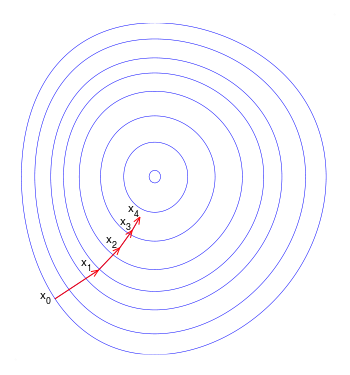
\includegraphics[width=0.5\textwidth]{Figures/gradientdescent.png}
\caption{The method of gradient descent iteratively approaches a global minimum on a convex function (\cite{gradientdescent}).}
\label{fig:gradientdescent}
\end{figure}

\subsubsection{Coordinate Descent}

Another plausible optimisation algorithm is coordinate descent, where each descent step optimises with respect to a single variable. For OLS regression we have,

$$
\frac{\delta\mathcal{L}(\boldsymbol\beta_k)}{\delta\boldsymbol\beta_k} = \frac{1}{N}\sum_{n=1}^N x_{ik}(y_i - \mathbf{x}_i^T\boldsymbol\beta)
\implies \beta_k^* = \frac{\sum_n x_{nk}y_n - \sum_n\sum_{j \neq k}x_{nk} x_{nj}\beta_j}{\sum_n x_{nk}^2}.
$$

\subsection{Model Prediction}

Once we have computed our optimal model parameters, $\boldsymbol\beta^*$, we can start making predictions for unseen data, $\hat{\mathbf{x}}$. Our prediction is then,

$$\hat{y} = \hat{\mathbf{x}}^T\boldsymbol\beta^*.$$

\subsection{Maximum Likelihood Estimation}

Now we will derive our regression model from a probabilistic angle. Probabilistic constructions are preferred in machine learning because they make the models more comprehensible\footnote{For some techniques, however, such as neural networks, things are not so straightforward.}. We start our derivation with the following assumptions: firstly, that the data points, $(\mathbf{x}_n, y_n)$ are independent and identically distributed (i.i.d); second, that the output variable is modelled by a linear function with Gaussian noise, that is, $\mathbf{y} = X\boldsymbol\beta + \boldsymbol\epsilon$, where $\boldsymbol\epsilon$ is a vector of normally distributed random variables, $\epsilon_i \sim \mathcal{N}(0, \sigma^2)$, for which $\sigma^2$ is the variance representing the random noise. We are thereby making an assumption about how the output variable is distributed around our line of best fit, $\mathbf{x}_n^T\boldsymbol\beta$. Now we may write a probability distribution for $y_n$,

$$p(y_n|\mathbf{x}_n, \boldsymbol\beta) = \mathcal{N}(\mathbf{x}_n^T\boldsymbol\beta, \sigma^2),$$

and since the data points are independent, the distribution over all $y_n$ is,

$$p(\mathbf{y}|X, \boldsymbol\beta) = \prod_{n=1}^N p(y_n|\mathbf{x}_n, \boldsymbol\beta).$$

As we will soon see, maximising this probability is equivalent to minimising the square loss function! Because of our assumption of Gaussian noise, the optimal parameters will be those that construct a hyperplane such that the data points around it are distributed according to a Normal distribution, that is, maximising the likelihood of the data around the plane. This is equivalent to minimising the square loss. As we shall see, it is convenient to work with the log of the likelihood. Since a $\log$ function is a monotonically increasing function, maximising the log-likelihood is no different to maximising the likelihood itself. Therefore we have,

\begin{align}
\max_{\boldsymbol\beta}\mathcal{L}_{lik}(\boldsymbol\beta) &= \max_{\boldsymbol\beta}\Big\{\log \prod_{n=1}^N \mathcal{N}(\mathbf{x}_n^T\boldsymbol\beta, \sigma^2)\Big\} \notag \\
&=\max_{\boldsymbol\beta}\Big\{\sum_{n=1}^N \log \frac{1}{\sigma\sqrt{2\pi}}e^{-(y - \mathbf{x}_n^T\boldsymbol\beta)^2/2\sigma^2}\Big\} \notag \\
&=\max_{\boldsymbol\beta}\Big\{-\frac{1}{2\sigma^2}\sum_{n=1}^N (y - \mathbf{x}_n^T\boldsymbol\beta)^2 + \log\frac{N}{\sigma\sqrt{2\pi}}\Big\} \notag \\
&=\max_{\boldsymbol\beta}\Big\{-k_1\mathcal{L}(\boldsymbol\beta) + k_2\Big\} \notag \\
&=\min_{\boldsymbol\beta}\mathcal{L}(\boldsymbol\beta)\notag
\end{align}

where $k_1$ and $k_2$ are positive constants, and so they have no bearing on the optimal $\boldsymbol\beta^*$. Thus, we see that maximising our likelihood function is equivalent to minimising our original mean square error loss function. This is equivalently known as the negative log-likelihood (NLL).

\subsection{Non-linear Fits}

If we wish to fit a non-linear function to our data, we can simply transform the data. For example, if we want to fit a quadratic function to our data (Figure \ref{fig:quadraticfit}), we need only square the values in our dataset and introduce it as a new dimension in our data. It is important to note that this is still a linear regression, as we still have a linear combination of parameters, albeit with a non-linear basis function. These more complex models are best created in the framework of a \emph{ridge regression}, where we introduce a penalty term in the loss function.

\begin{figure}[!ht]
\centering
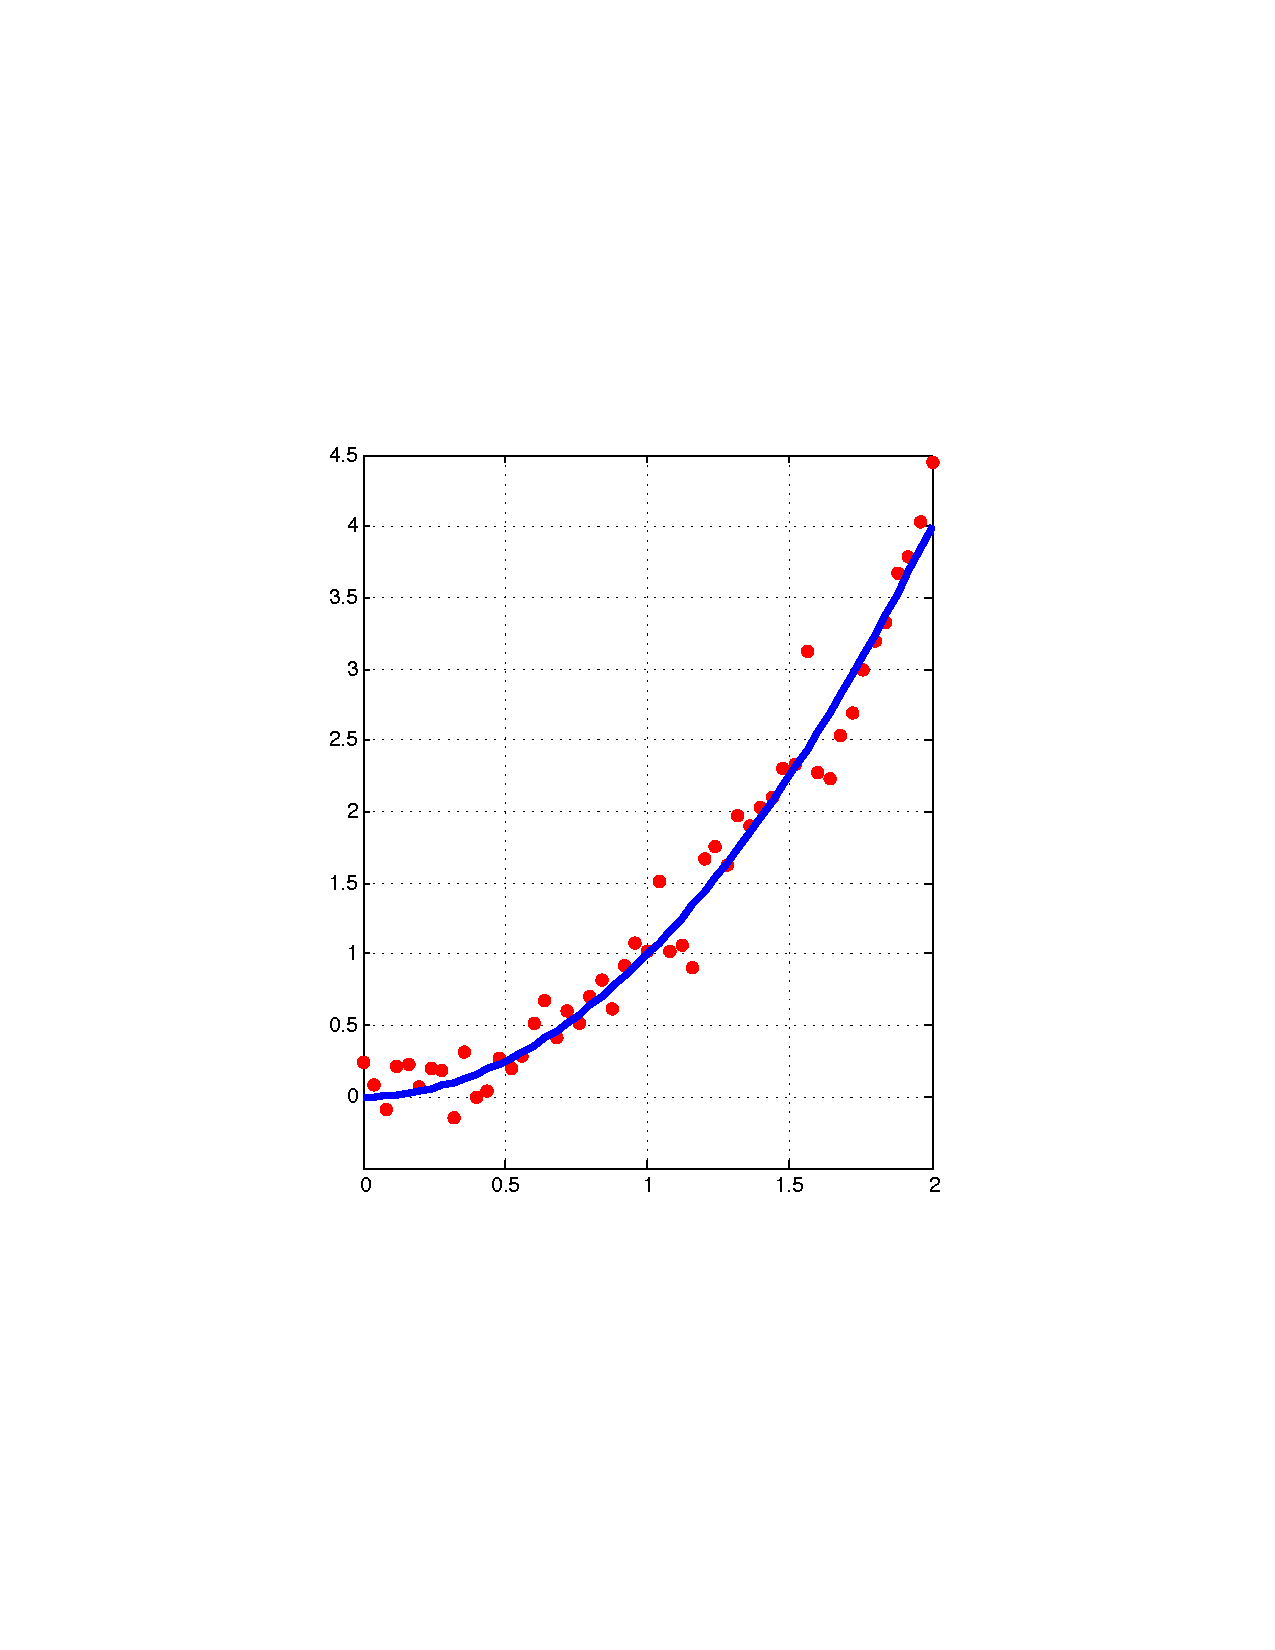
\includegraphics[width=0.5\textwidth]{Figures/quadraticfit.pdf}
\caption{A non-linear fit may be found by transforming the data with a non-linear basis function.}
\label{fig:quadraticfit}
\end{figure}

\subsection{Bayesian Linear Regression}

Bayes model averaging may be performed for linear regression to obtain a more robust posterior predictive distribution, just as we saw for generative classifiers. Such a result can for example be analysed for its variance, unlike a mere point estimate such as ML or MAP estimates. The derivation involves multiplying and integrating Gaussians and belongs in a textbook, rather than in Last Chance Stats.

\subsection{Robust Linear Regression}

One drawback of using a Gaussian likelihood is that it is sensitive to outliers. This makes it likely to overfit in practice. There are several ways of mitigating this effect. The most crude is known as `early stopping', where training is terminated before convergence, and before the model has a chance to overfit. The most ideal option is to train on more data, taking density away from outliers, but data is usually hard to come by. The most common approach is to \emph{regularise} the cost function by introducing a prior distribution on the model parameters. This gives us the posterior distribution, just as it was with the beta-binomial model, and the optimal parameters are the MAP estimate, $\boldsymbol\theta_{MAP} = \argmax_{\boldsymbol\theta} \text{NLL}(\boldsymbol\theta)$, where NLL is the negative log-likelihood. If we choose another Gaussian for the prior, we are using $l_2$ regularisation, and we get what is known as a \emph{ridge regression},

$$\text{NLL} = \frac{1}{2}(\mathbf{y} - \mathbf{X}\boldsymbol\beta)^T(\mathbf{y} - \mathbf{X}\boldsymbol\beta) + \frac{\lambda}{2}\boldsymbol\beta^T\boldsymbol\beta = \frac{1}{2}\sum_{n=1}^N(y_n - \boldsymbol\beta^T\mathbf{x}_n)^2 + \frac{\lambda}{2}\sum_{d=1}^D\beta_d^2.$$

Clearly, this is a linear regression with an extra cost over the parameter values. This is known as a penalty term in the cost function. High parameter values, which correspond to more complex fits (overfitting), are punished with a quadratic cost. The parameter $\lambda$ is a scaling constant which may be optimised through cross-validation. Ridge regression is very popular, and has the added bonus of producing a more numerically stable normal equation, because the regularisation term increases the eigenvalues of the gram matrix, $\mathbf{X^T}\mathbf{X}$, in the normal equations, thereby reducing the ratio between the highest and lowest eigenvalues, and thereby improving its condition number. Another option is a Laplace prior. This is known as $l_1$ regularisation, and when applied to regression is known as a LASSO\footnote{Least absolute shrinkage and selection operator} regression. One of the effects of $l_1$ regularisation is to encourage \emph{sparse} models. Sparsity refers to models whose parameters are non-zero for only a small subset of the dimensions. Encouraging sparsity is a form of \emph{feature selection}. This is useful for high-dimensional data with many noisy indicators, otherwise known as the `small $N$, large $D$' problem. The intuition behind this phenomenon of encouraging sparsity is that the contours of the prior distribution are linear, forming a diamond shape in the parameter space, whose vertices lie along each of the axes. In contrast, the Gaussian $l_2$ prior has ellipsoidal contours. Thus, in $l_1$ regularisation sparse parameters on the axes have greater magnitude than parameters along the edges of the diamond. These sparse parameters with greater magnitude (allowing for better fits) may be chosen at no extra penalty. Unfortunately, the cost function is no longer differentiable everywhere, due to the absolute value function, and our solution algorithm changes--the most common approaches are coordinate descent algorithms\footnote{Coordinate descent algorithms are similar to gradient descent, but where at each step the function is optimised with respect to one variable.} such as the `shooting' algorithm.

A final, more drastic option for robust regression is to modify the form of the likelihood to a distribution with heavier tails, making it more robust to outliers, thereby creating to \emph{robust linear regression}. Typical choices are the Student or Laplace distributions. In the latter case, the function is convex but no longer differentiable, but with a reformulation trick can be made into a linear programming problem. For example, given a Laplace likelihood,

$$\text{NLL}(\mathbf{w}) \propto -\log\prod_n\exp\big({-|y_n- \mathbf{w}^T\mathbf{x}_n|}\big) = \sum_n |y_n- \mathbf{w}^T\mathbf{x}_n|.$$

We can remove the absolute value sign using the \emph{split variable trick}, that is, by introducing artificial positive and negative variables, $r_n^+$ and $r_n^-$, such that,

$$\text{NLL}(\mathbf{w}) =  \sum_n r_n^+ + r_n^-,$$

where $r_n^+ - r_n^- = y_n- \mathbf{w}^T\mathbf{x}_n$ with the \emph{type} constraint that $r_n^+r_n^- = 0$ (ensuring only one variable is activated at a time), and $r_n^+, r_n^- \geq 0$. The type constraint can be omitted, as at optimality it will be satisfied as a matter of course. Now we have a constrained convex optimisation problem, which can be optimised with any linear solver, for example, the simplex algorithm.

\section{The Simplex Algorithm}

The simplex algorithm was designed by American mathematician George Dantzig\footnote{There is a famous anecdote from Dantzig's time as a doctoral student at Berkeley. Arriving late to class, Dantzig copied down two important unsolved statistics problems the professor had earlier written on the blackboard, taking them to be set for homework. With some effort, he managed to solve both problems, and submitted them to the professor for review. It was not until some weeks later that the professor looked at the solutions, to his amazement. Dantzig later had the rare privilege of submitting his homework as his doctoral thesis.} (1914-2005). It is an optimisation algorithm for linear programming problems, that is, a problem of the form,

\begin{align}
\begin{array}{rl}
\text{maximise} & z = \mathbf{c}^T\mathbf{x} \\
\text{subject to} & \mathbf{A}\mathbf{x} = \mathbf{b}, x_i \geq 0
\end{array}
\label{eq:linprog}
\end{align}

where $z$ is known as the objective function, and the linear system specifies a set of linear constraints on the values of the input variables, $x_i$, which are further non-negative. The program specifies an N-dimensional convex solid\footnote{If we take a spherical fruit such as an apple to be our unconstrained convex function, adding a linear constraint corresponds to slicing it at some position at a fixed angle. Intuitively, the fruit remains convex after the cut, despite losing its smoothness (roundness).}, and the algorithm works by moving along the edges of this shape from corner to corner. As any optimal solution must be on the surface, we can discard all points interior to the solid. This reduces the feasible solution space to a finite set. Furthermore, the convexity of the solid guarantees that as long as we repeatedly take upward steps along the surface edges, we will arrive at a maximum in a finite number of steps. In practice the algorithm is very efficient, though there are a special class of problems for which the algorithm will run in exponential time. Now, take for example the simple program,

$$
\begin{array}{rl}
\text{maximise} & z = 2x_1 + x_2 \\
\text{subject to} & x_1 + x_2 \leq 5 \\
& 5x_1 + 2x_2 \leq 10 \\
& x_1, x_2 \geq 0
\end{array},
$$

\begin{figure}[!ht]
\centering
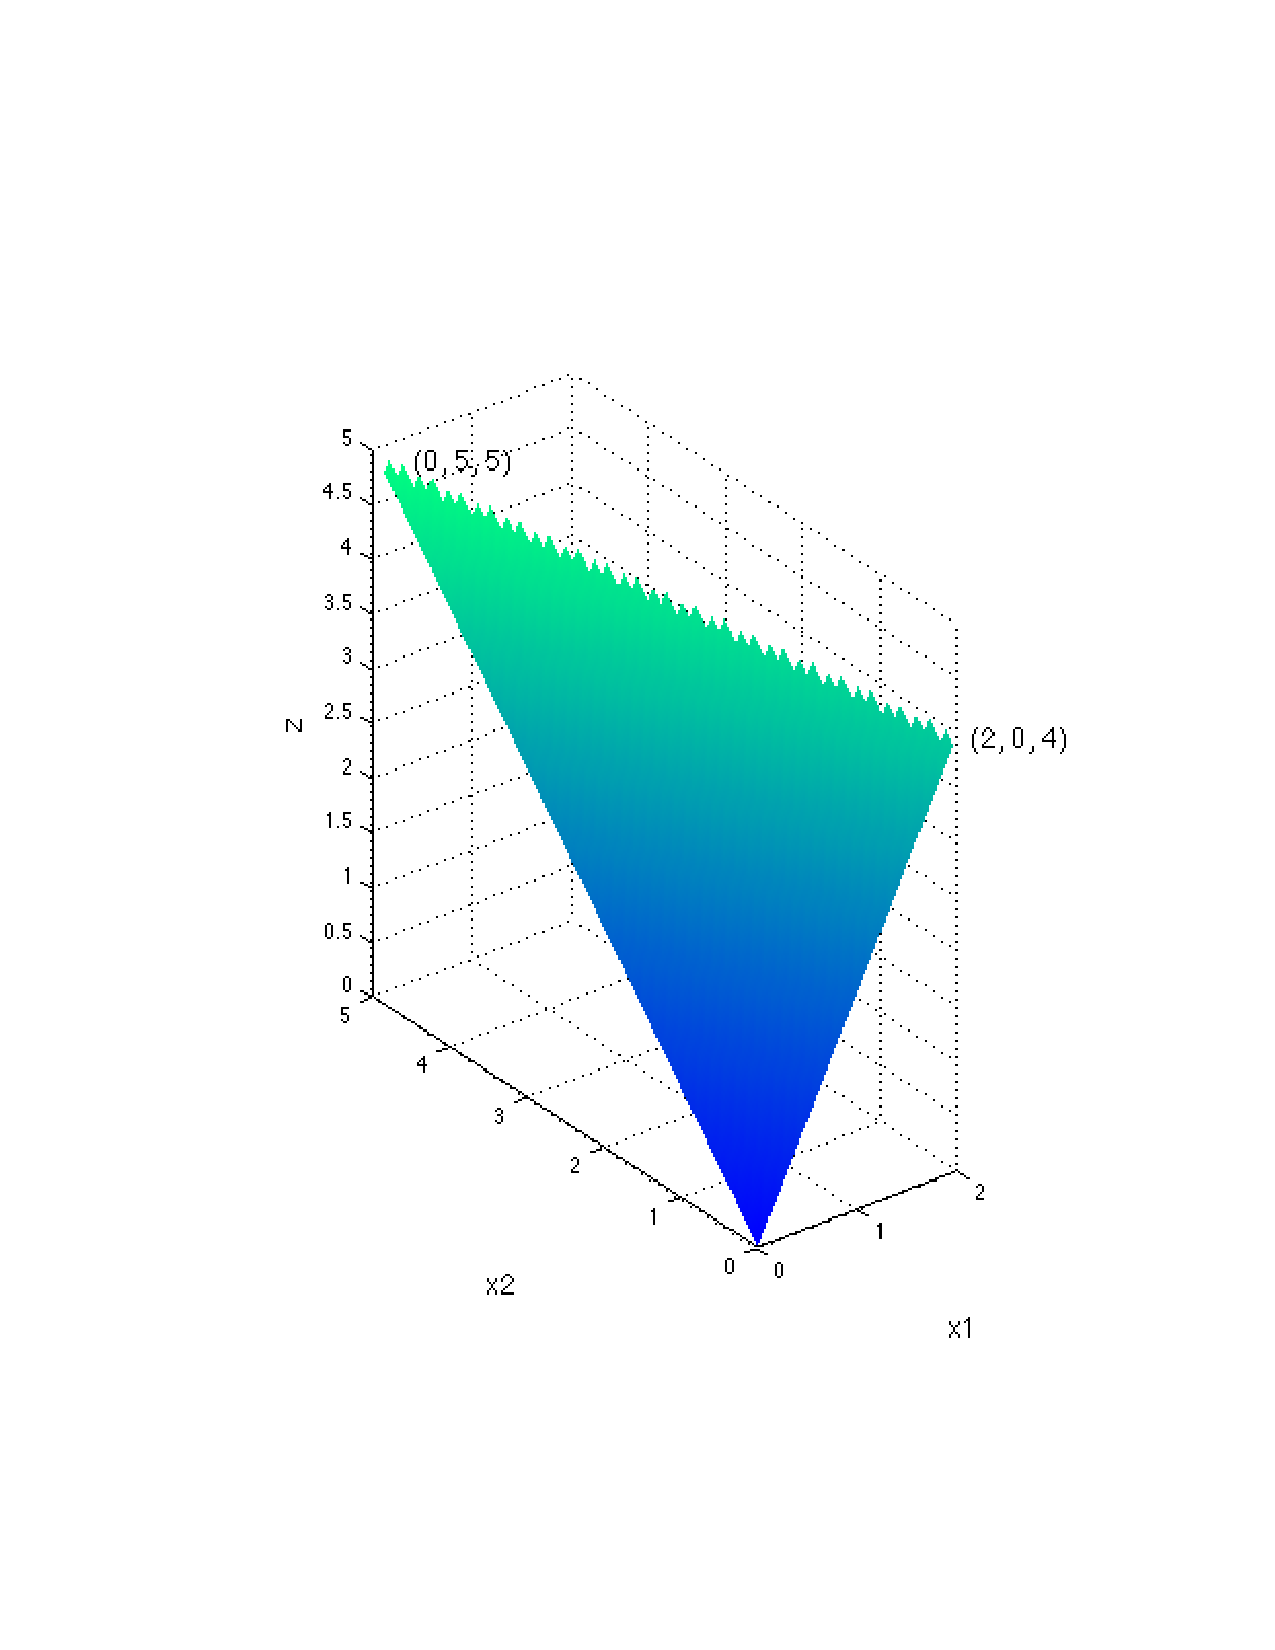
\includegraphics[width=0.5\textwidth]{Figures/simplex.pdf}
\caption{The convex surface of a simple linear programming problem.}
\label{fig:simplex}
\end{figure}


depicted in Figure \ref{fig:simplex}. The first phase of optimisation involves reformulating the linear program into the \emph{standard} form expressed in (\ref{eq:linprog}). First, any unrestricted variables are eliminated from the program. Then, any variable with a non-zero lower bound is replaced with a variable specifying an offset. Finally, \emph{slack} variables are introduced to change any inequality constraint to an equality constraint. In our problem, two slack variables are required giving,

$$
\begin{array}{rl}
\text{maximise} & z = 2x_1 + x_2 \\
\text{subject to} & x_1 + x_2 + s_1 = 5 \\
& 5x_1 + 2x_2 + s_2 = 10 \\
& x_1, x_2, s_1, s_2 \geq 0
\end{array}.
$$

The convenient way to apply the algorithm is to write the problem into a \emph{tableau}. This can be written,

$$
\begin{array}{rrrrr|r}
x_1&x_2&s_2&s_2&z&c \\
\hline
1&1&1&0&0&5 \\
\mathbf{5}&2&0&1&0&10 \\
\hline
-2&-1&0&0&1&0 \\
\end{array}
$$

The tableau form permits the execution of the algorithm to follow a sequence of simple row reductions. We begin by considering the final line of the tableau. This indicates the rate of increase of the objective function with respect to a change in each variable. As a simple heuristic, we select the variable yielding the greatest increase: $x_1$. We then select the constraint that most restricts increasing this variable--here, the second. The choice of row and column defines the \emph{pivot} variable for the current iteration. The task now is to render the $x_1$ column an elementary vector with the unit in the pivot position. This can be achieved first by scaling the second row by $1/5$ ($R_2^* \leftarrow \frac{1}{5}R_1 $), then subtracting it from the first row ($R_1^* \leftarrow R_1 - R_2^*$), and adding twice that to the final row ($R_3^* \leftarrow R_3 + 2R_2^*$), yielding,

$$
\begin{array}{rrrrr|r}
x_1&x_2&s_2&s_2&z&c \\
\hline
0&\mathbf{3/5}&1&-1/5&0&3 \\
1&2/5&0&1/5&0&2 \\
\hline
0&-1/5&0&2/5&0&4 \\
\end{array}
$$

Now we are at a point on the surface $(2, 0, 4)$ at which increases in $x_1$ yield $0$ improvement to $z$. Hence, we are at a corner on the surface. The presence of negative coefficients in the final row indicates further improvement can be made. Identifying the next pivot element and repeating the process gives,

$$
\begin{array}{rrrrr|r}
x_1&x_2&s_2&s_2&z&c \\
\hline
0&1&5/3&-1/3&0&5\\
1&0&-2/3&1/3&0&0\\
\hline
0&0&1/3&-1/15&0&5\\
\end{array}
$$

Now we see the final row contains non-negatives for $x_1$ and $x_2$, therefore no improvement can be made by varying either variable, and hence we have arrived at an optimal solution. Because the state of $R_3$ (the objective function) has been arrived at as a combination of its previous state and the new first constraint, $R_1$, any solution which satisfies the under-determined $R_1$ satisfies its contribution to $R_3$. Hence, we choose the trivial solution, $(x_1, 5, 0, 0, 0)$. This may not always be the only optimal solution (though in our problem it is), but it is indeed optimal. Because of the linearly independent basis vectors, this leaves the trivial solution available in the second constraint, $R_2$, that is, $(0, x_2, 0, 0, 0)$. Combining these yields the optimal solution, $x_1 = 0, x_2 = 5, s_1 = 0, s_2 = 0$, as seen in Figure \ref{fig:simplex}. Thus, in general, our method brings us to a state wherein the optimal solution can be read directly from the final tableau as the basic columns, with other variables equal to 0. As noted, this method verifiably gives us an optimal solution, though others may exist.

\section{Logistic Regression}

Logistic regression is a class of classification models. Learning a logistic regression can be thought of as fitting a multivariate Bernoulli distribution. There is also a strong connection between logistic regression and linear discriminant analysis. In fact, logistic regression models are the \emph{discriminative} form of the same model. Discriminative models fit a posterior predictive distribution directly, unlike generative models, which derive the posterior by combining likelihood and prior distributions\footnote{This is often hard to do, especially when the input data is vector-valued, and is a limitation on generative models. In contrast, discriminative models allow for arbitrary basis function expansion and feature engineering. On the other hand, generative models are usually easier to fit, more robust to changes in the dataset (discriminative models must be retrained), and better facilitate semi-supervised learning.}. Logistic regressions are a core part of machine learning with ties to more sophisticated techniques such as neural networks. Studying logistic regressions notably presents the student with the quintessential optimisation techniques of machine learning. Linear and logistic regressions are part of a wider family of models called \emph{generalised linear models} (GLM). This is a family of models modeling exponential densities over output variables, and where the mean is a linear combination of the parameters, in some cases passed through a non-linear function. A GLM can be characterised by a choice of probability distribution and a choice of \emph{link function}. In OLS regression, this link function is the identity; in logistic regression it is the logistic function. In a \emph{poisson regression}, the poisson distribution is used with a $\log$ link function. In this case, applying maximum likelihood gives a convex differentiable function and the regression may be performed with gradient descent. Recall a poisson distribution models the number of occurrences of an event with a given occurrence rate over a given time period. In the same way a logistic regression is more suitable for classification than OLS, a poisson regression is more suitable for modeling \emph{rates}.

\subsection{Binary Logistic Regression}

A binary logistic regression models,

$$p(y|\mathbf{x}, \boldsymbol\beta) = \text{Ber}(y|\sigma(\boldsymbol\beta^T\mathbf{x})),$$

where,

$$\sigma(\boldsymbol\beta^T\mathbf{x}) = \frac{\exp(\boldsymbol\beta^T\mathbf{x})}{1 + \exp(\boldsymbol\beta^T\mathbf{x})},$$

is the sigmoid or logistic function\footnote{This may be substituted by any function mapping $(-\infty, +\infty) \to [0, 1]$, for example the Gaussian CDF, giving what is known as a \emph{probit} regression. Recall these functions have roughly the same shape, but a Gaussian CDF may also be tuned by its variance.}. Thus, in training a logistic regression model we are fitting a multivariate Bernoulli distribution. In this binary case, we encode the class variable as a binary variable, that is, $y_i \in \{0, 1\}$, and we have $p(y = 1) = \sigma(\boldsymbol\beta^T\mathbf{x})$ and $p(y = 0) = 1 - \sigma(\boldsymbol\beta^T\mathbf{x})$. The negative log likelihood for our model is therefore,

\begin{align}
\text{NLL}(\boldsymbol\beta) &= -\log\prod_i \sigma(\boldsymbol\beta^T\mathbf{x}_i)^{y_i}(1 - \sigma(\boldsymbol\beta^T\mathbf{x}_i))^{(1 - y_i)} \notag \\
&= \sum_i \log(1 + \exp(\boldsymbol\beta^T\mathbf{x}_i)) - y_i\boldsymbol\beta^T\mathbf{x}_i.\notag
\end{align}

Due to the logistic function, it is no longer possible to obtain a least-squares solution. We therefore have recourse to numerical techniques.

\subsubsection{Newton's method}

Because the function is convex, vanilla gradient descent will do the trick. However, more powerful techniques exist. Newton's method\footnote{This is a multivariate generalisation of the Newton root-finding method. Here, however, we are finding the ``root'' of the gradient.} is a similar algorithm incorporating second order information into the descent step. It comes from considering the second order Taylor polynomial for the NLL function, around a point $\boldsymbol\beta_k$,

$$NLL(\boldsymbol\beta) \approx NLL(\boldsymbol\beta_k) + g_k^T(\boldsymbol\beta - \boldsymbol\beta_k) + \frac{1}{2}(\boldsymbol\beta - \boldsymbol\beta_k)\mathbf{H}_k(\boldsymbol\beta - \boldsymbol\beta_k).$$

This quadratic expression is minimised for $\boldsymbol\beta = \boldsymbol\beta_k - \mathbf{H}^{-1}g_k$. This constitutes the Newton descent step. Now we will derive expressions for the gradient and Hessian of our logistic regression model. The gradient is the vector of partial derivatives,

$$g(\boldsymbol\beta) = \begin{bmatrix}
\frac{\partial}{\partial \beta_0} \text{NLL}(\boldsymbol\beta) \\
\frac{\partial}{\partial \beta_1} \text{NLL}(\boldsymbol\beta) \\
\vdots \\
\frac{\partial}{\partial \beta_D} \text{NLL}(\boldsymbol\beta) \\
\end{bmatrix} =
\sum_i \begin{bmatrix}
(\sigma(\boldsymbol\beta\mathbf{x}_i) - y_i)x_{i1} \\
(\sigma(\boldsymbol\beta\mathbf{x}_i) - y_i)x_{i2} \\
\vdots \\
(\sigma(\boldsymbol\beta\mathbf{x}_i) - y_i)x_{iD} \\
\end{bmatrix}
= \sum_i (\sigma_i - y_i)\mathbf{x}_i = \mathbf{X}^T(\boldsymbol\sigma - \mathbf{y}),
$$

The Hessian is defined as $\frac{\partial}{\partial\mathbf{\boldsymbol\beta}}g(\boldsymbol\beta)^T$,

$$\mathbf{H} = \begin{bmatrix}
\frac{\partial}{\partial \beta_0} g(\boldsymbol\beta) \\
\frac{\partial}{\partial \beta_1} g(\boldsymbol\beta) \\
\vdots \\
\frac{\partial}{\partial \beta_D} g(\boldsymbol\beta) \\
\end{bmatrix} =
\sum_i\begin{bmatrix}
\sigma(\boldsymbol\beta\mathbf{x}_i)(1 - \sigma(\boldsymbol\beta\mathbf{x}_i))x_{i1}\mathbf{x}_i^T \\
\sigma(\boldsymbol\beta\mathbf{x}_i)(1 - \sigma(\boldsymbol\beta\mathbf{x}_i))x_{i2}\mathbf{x}_i^T \\
\vdots \\
\sigma(\boldsymbol\beta\mathbf{x}_i)(1 - \sigma(\boldsymbol\beta\mathbf{x}_i))x_{iD}\mathbf{x}_i^T
\end{bmatrix}
= \sum_i \sigma_i(1 - \sigma_i)\mathbf{x}_i\mathbf{x}_i^T = \mathbf{X}^T\mathbf{S}\mathbf{X},
$$

where $S = \text{diag}([\sigma(\boldsymbol\beta^T\mathbf{x}_1), \sigma(\boldsymbol\beta^T\mathbf{x}_2), \dots, \sigma(\boldsymbol\beta^T\mathbf{x}_N)])$. The Newton step may be rewritten as a least squares problem. In such a formulation, the optimisation algorithm is known as iterative reweighted least squares (IRLS).

\subsubsection{BFGS}

Due to the computational complexity of computing the Hessian, quasi-Newton techniques exist that create an approximation iteratively. The most common quasi-Newton method is the BFGS algorithm (Broyden, Fletcher, Goldfarb and Shanno). It is quasi-Newton because it relies on the secant equation\footnote{Similar to the fact that Newton's method is a generalisation of the Newton root-finding method, BFGS is approximates a multivariate generalisation of the secant root-finding method.},

\[
\mathbf{H_{k+1}}(\mathbf{x_{k+1}} - \mathbf{x_k}) = \mathbf{g}_{k+1} - \mathbf{g}_k,
\]

which is true in the limit, but only approximately true for a step of $\mathbf{x_{k+1}} - \mathbf{x_k}$. BFGS makes an update to the Hessian at each iteration,

$$H_{k+1} = H_k + \alpha\mathbf{u}\mathbf{u}^T + \beta\mathbf{v}\mathbf{v}^T,$$

equating to two rank-one updates (hence a rank-two update overall). The vectors $\mathbf{u}$ and $\mathbf{v}$ are chosen such that the secant equation is satisfied. This approximation makes the Hessian cheaper to compute and to invert. Particularly when the Hessian is sparse, BFGS can greatly speed up Newton's method.

The $\mathcal{O}(D^2)$ space complexity of the Hessian gives rise to a further approximation in the limited memory or L-BFGS algorithm. This is the usual weapon of choice for modeling high-dimensional data. Just as with linear regression, $l_2$ regularisation may be used. Unlike linear regression, however, the full posterior distribution is not directly computable due to the absence of a conjugate prior. Approximation techniques, such as Markov chain Monte Carlo (MCMC), are therefore used. An object-oriented logistic regression model is solved with both gradient descent and Newton's method in \texttt{logRegDemo.m}.

\subsection{Multinomial Logistic Regression}

Going beyond binary logistic regression requires some adjustments--the sigma function is replaced by the generalised softmax function,

$$p(y_i = c | \mathbf{x}_i, \mathbf{W}) = \frac{\exp(\mathbf{w}_c^T\mathbf{x})}{\sum_{c' = 1}^C \exp(\mathbf{w}_{c'}^T\mathbf{x})},$$

just as with linear discriminant analysis\footnote{Clearly, the sigma function is the simplified binary form of the softmax function.}. We now have the generalised multinomial or softmax regression. The parameters now make up a matrix $\mathbf{W}$ whose $C$ columns correspond to each of the $C$ classes\footnote{This, incidentally leads to an identifiability issue. Identifiability is a property of statistical models whereby a model (the distribution) is defined by a unique parameter set, that is, there is a one-to-one mapping between parameters and models. It is important for precise statistical inference. In this instance the model is clearly not identifiable, as adding any constant vector to each of the parameter vectors gives the same model probabilities. To address this, the parameters are usually offset to eliminate the ambiguity.}. Note that the matrix structure is only for notational convenience, the parameters still effectively constitute a vector of unknowns, and the gradient still has a vector structure. The binary encoding on the classes is dropped in favour of a `one-of-C encoding' binary vector of length $C$. Thus, the negative log likelihood is,

$$\text{NLL}(\mathbf{W}) = -\sum_i \bigg[\bigg(\sum_{c = 1}^Cy_{ic}\mathbf{w}_c^T\mathbf{x}_i\bigg) - \log\bigg(\sum_{c'=1}^C\exp(\mathbf{w}_{c'}^T\mathbf{x}_i)\bigg)\bigg].$$

The gradient and Hessian may be derived as before, but it useful to introduce a specialised \emph{Kronecker\footnote{Leopold Kronecker (1823-1891) was a German mathematician, well known for his Kronecker delta--a shorthand for the indicator function for identity. This is not to be confused with the Dirac delta function, a Gaussian distribution with infinitesimal variance.} tensor product} notation for specifying block matrices,

$$\mathbf{A} \otimes \mathbf{B} = \begin{bmatrix}
a_{11}\mathbf{B}&a_{12}\mathbf{B}&\cdots&a_{1m}\mathbf{B}\\
a_{21}\mathbf{B}&a_{22}\mathbf{B}&\cdots&a_{2m}\mathbf{B}\\
\vdots & \vdots & \ddots & \vdots \\
a_{n1}\mathbf{B}&a_{n2}\mathbf{B}&\cdots&a_{nm}\mathbf{B}\\
\end{bmatrix}.$$

Now, we may derive the gradient as before, adhering to the first principle of forming the vector of partial derivatives,

$$g(\mathbf{W}) = \begin{bmatrix}
\frac{\partial}{\partial \mathbf{w}_{11}} \text{NLL}(\mathbf{W}) \\
\vdots \\
\frac{\partial}{\partial \mathbf{w}_{D, C}} \text{NLL}(\mathbf{W}) \\
\end{bmatrix} =
\sum_i \begin{bmatrix}
(\sigma(\mathbf{w}_1\mathbf{x}_i) - y_{i1})x_{i1} \\
\vdots \\
(\sigma(\mathbf{w}_c\mathbf{x}_i) - y_{ic})x_{iD} \\
\end{bmatrix}
= \sum_i (\boldsymbol\sigma_i - \mathbf{y}_i)\otimes\mathbf{x}_i.
$$

The Hessian is seemingly messy to derive, but it can be done on paper without too much trouble\footnote{It is simplest to try the 2-dimensional case with two classes to spot the pattern.}, yielding,

$$\mathbf{H}(\mathbf{W}) =  \begin{bmatrix}
\frac{\partial}{\partial \mathbf{w}_{11}} g(\mathbf{W}) \\
\vdots \\
\frac{\partial}{\partial \mathbf{w}_{D, C}} g(\mathbf{W}) \\
\end{bmatrix} = \sum_i (\text{diag}(\boldsymbol\sigma_i) - \boldsymbol\sigma_i\boldsymbol\sigma_i^T)\otimes(\mathbf{x}_i\mathbf{x}_i^T),$$

giving a $DC \times DC$ matrix. The model can likewise incorporate a regularisation term. An example of multinomial logistic regression is given in \texttt{logRegDemo.m}.

\section{Online Learning and Perceptrons}

\subsection{Online learning}
Online learning is an alternative to the more customary offline learning. In online learning, data is streamed rather than processed in a batch. That is, data samples arrive one at a time, and the parameters are adjusted at each iteration. The loss is compared to the batch performance in a function known as the \emph{regret}. This leads to a technique known as online gradient descent. It is further possible to simulate online learning as an alternative to batch gradient descent in an algorithm known as \emph{stochastic} gradient descent (SGD). Here, the gradient at a point is constructed on some subset of the available data, possibly a single data sample alone, rather than the full dataset. The algorithm cycles through the dataset in these smaller chunks, according to some random permutation. A complete cycle is known as an \emph{epoch}, and multiple epochs may be required before convergence is reached. There are various problems where it may be beneficial to do this, for example when fitting neural networks whose cost function is not convex. In this case, the randomness of stochastic gradient descent can help escape local minima during the descent. Moreover, the algorithm may simply outperform batch gradient descent, as calculating the full gradient is $\mathcal{O}(N^2)$, but only $\mathcal{O}(N)$ when a single sample is used. It is likely that a small subset of the data can give a good approximation to the true gradient, in particular when duplication is present in the data. When applied to least squares, the algorithm is known as least mean squares (LMS). A comparison of batch and stochastic gradient descent is given in \texttt{regressionDemo.m}.

\subsubsection{The Perceptron}
The perceptron is an historically important algorithm. It is one of the earliest machine learning algorithms, invented by American psychologist, Frank Rosenblatt (1928-1971), in 1956. The perceptron learns a binary classifier in an online manner from supervised data, in a process that closely resembles stochastic gradient descent\footnote{The perceptron algorithm replaces the probability, $\mu_i = p(y_i = 1 | \mathbf{x}_i)$, with the prediction, $\hat{y}_i$ (effectively rounding the probability), but is otherwise identical to SGD.}. The algorithm is guaranteed to converge if the data is linearly separable, and there is a nice proof of this. The algorithm is furthermore guaranteed \emph{not} to converge when the data is not linearly separable, and various enhancements exist to mitigate this problem. Notable examples of the perceptron's limitations are in learning logical functions. A perceptron can learn the \texttt{OR}, \texttt{AND}, and \texttt{NAND} functions, but is unable to learn \texttt{XOR}\footnote{Consider the four points arising from \texttt{XOR} in two variables--they are clearly not linearly separable.}. The multi-layer perceptron, also known as an artificial feed-forward neural network, arises from stacking several perceptrons in layers. These neural networks are much more flexible than the basic perceptron. The perceptron is also the origin of logistic regression, and maximum margin methods such as support vector machines (SVM). An example of a perceptron fitting the logical \texttt{NAND} function is given in \texttt{perceptronDemo.m}.

\section{Neural Networks}

Many types of neural networks exist\footnote{See for instance auto-encoders, which reconstruct the input from a reduced number of hidden states--a form of unsupervised learning; or convolutional neural networks, a neural network with a sliding window designed for pattern recognition within high resolution images.}, but we will consider the most common--the feed-forward neural network. Neural networks extend the structure of the simple perceptron by stacking a number of perceptrons into $K$ layers, such that the output of each layer propagates into the next. For this reason, a feed-forward neural network is also known as a \emph{multi-layer perceptron}. Each layer, $k$, has a number of `hidden' units, $\mathbf{z}^{(k)}$, and is a linear combination of the last layer of variables, $\mathbf{z}^{(k-1)}$, and a set of weights, $\mathbf{B}^{(k-1)}$, finally passed through a non-linear `activation' function, $h$\footnote{Classic choices are the sigma function or hyperbolic tangent function, itself a linear transform of the sigma function. The rectified linear unit (ReLU), the $\max$ function, and variations thereof are increasingly popular.}. That is, $\mathbf{z}^{(k+1)} = h(\mathbf{B}^{(k)}\mathbf{z}^{(k)})$ In this way, the states of each of the hidden units are a culmination of the previous layers. Thus, a neural network makes a prediction as,

$$\hat{y} = h(\mathbf{B}^{(K-1)}h(\mathbf{B}^{(K-2)}(\cdots(h(\mathbf{B}^{(1)})\hat{\mathbf{x}})))).$$

A neural network may be used for both regression and classification, the output passed through the logistic function in the latter case. Despite the complexity, this model can be trained with standard gradient descent techniques. There are some complications however, as the loss function is not convex. The gradients, $\frac{\partial\mathcal{L}}{\partial\mathbf{B}^{(k)}}$, are obtained by application of the chain rule, in an algorithm called \emph{back propagation}. Feed-forward neural networks, and other variants, have seen a great amount of success, especially with the advent of deep learning in recent years. Neural networks are very powerful non-linear models, which are in fact capable of fitting any smooth function given enough layers, making them \emph{universal approximaters}. A simple example of a neural network fitting an absolute value function is given in Figure \ref{fig:universalapproximater}.

\begin{figure}
\centering
\begin{tabular}{cc}
\subfloat[]{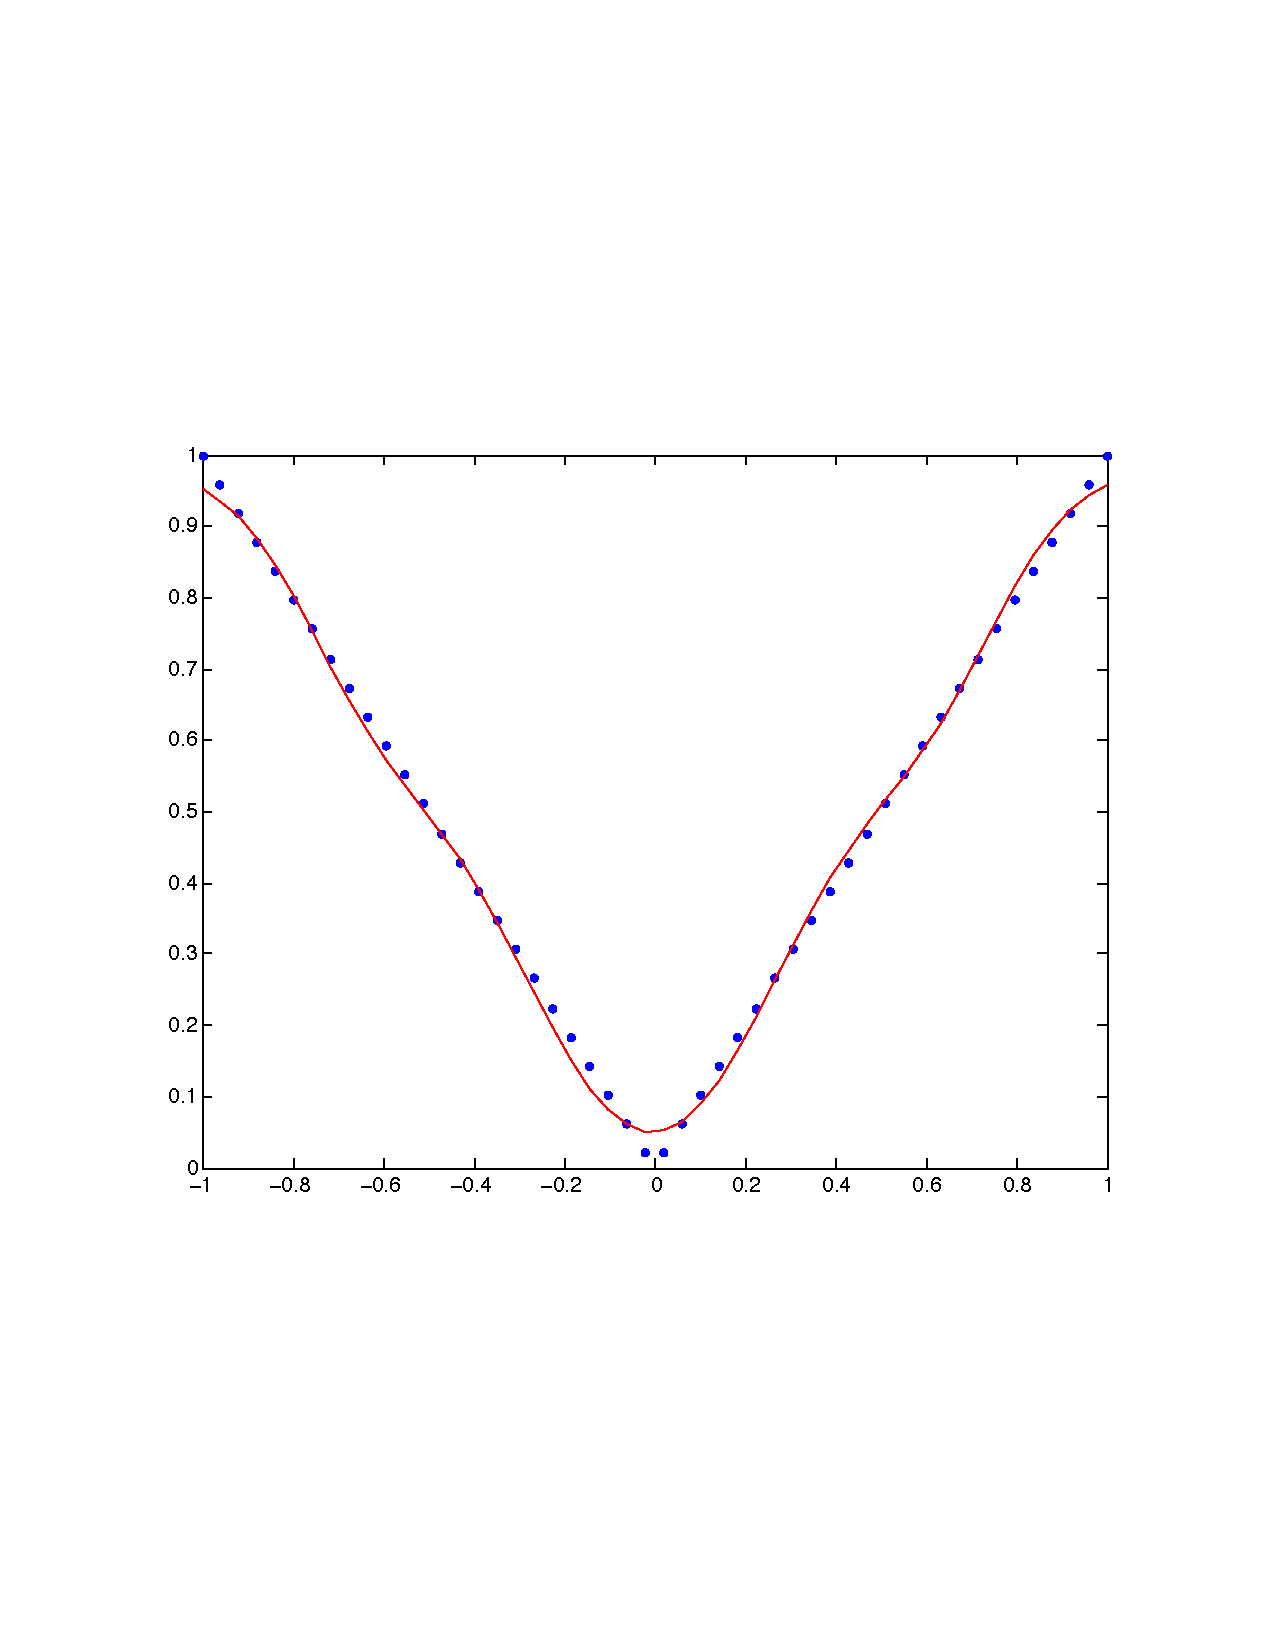
\includegraphics[width=0.49\textwidth]{Figures/universalapproximater.pdf}} & 
\subfloat[]{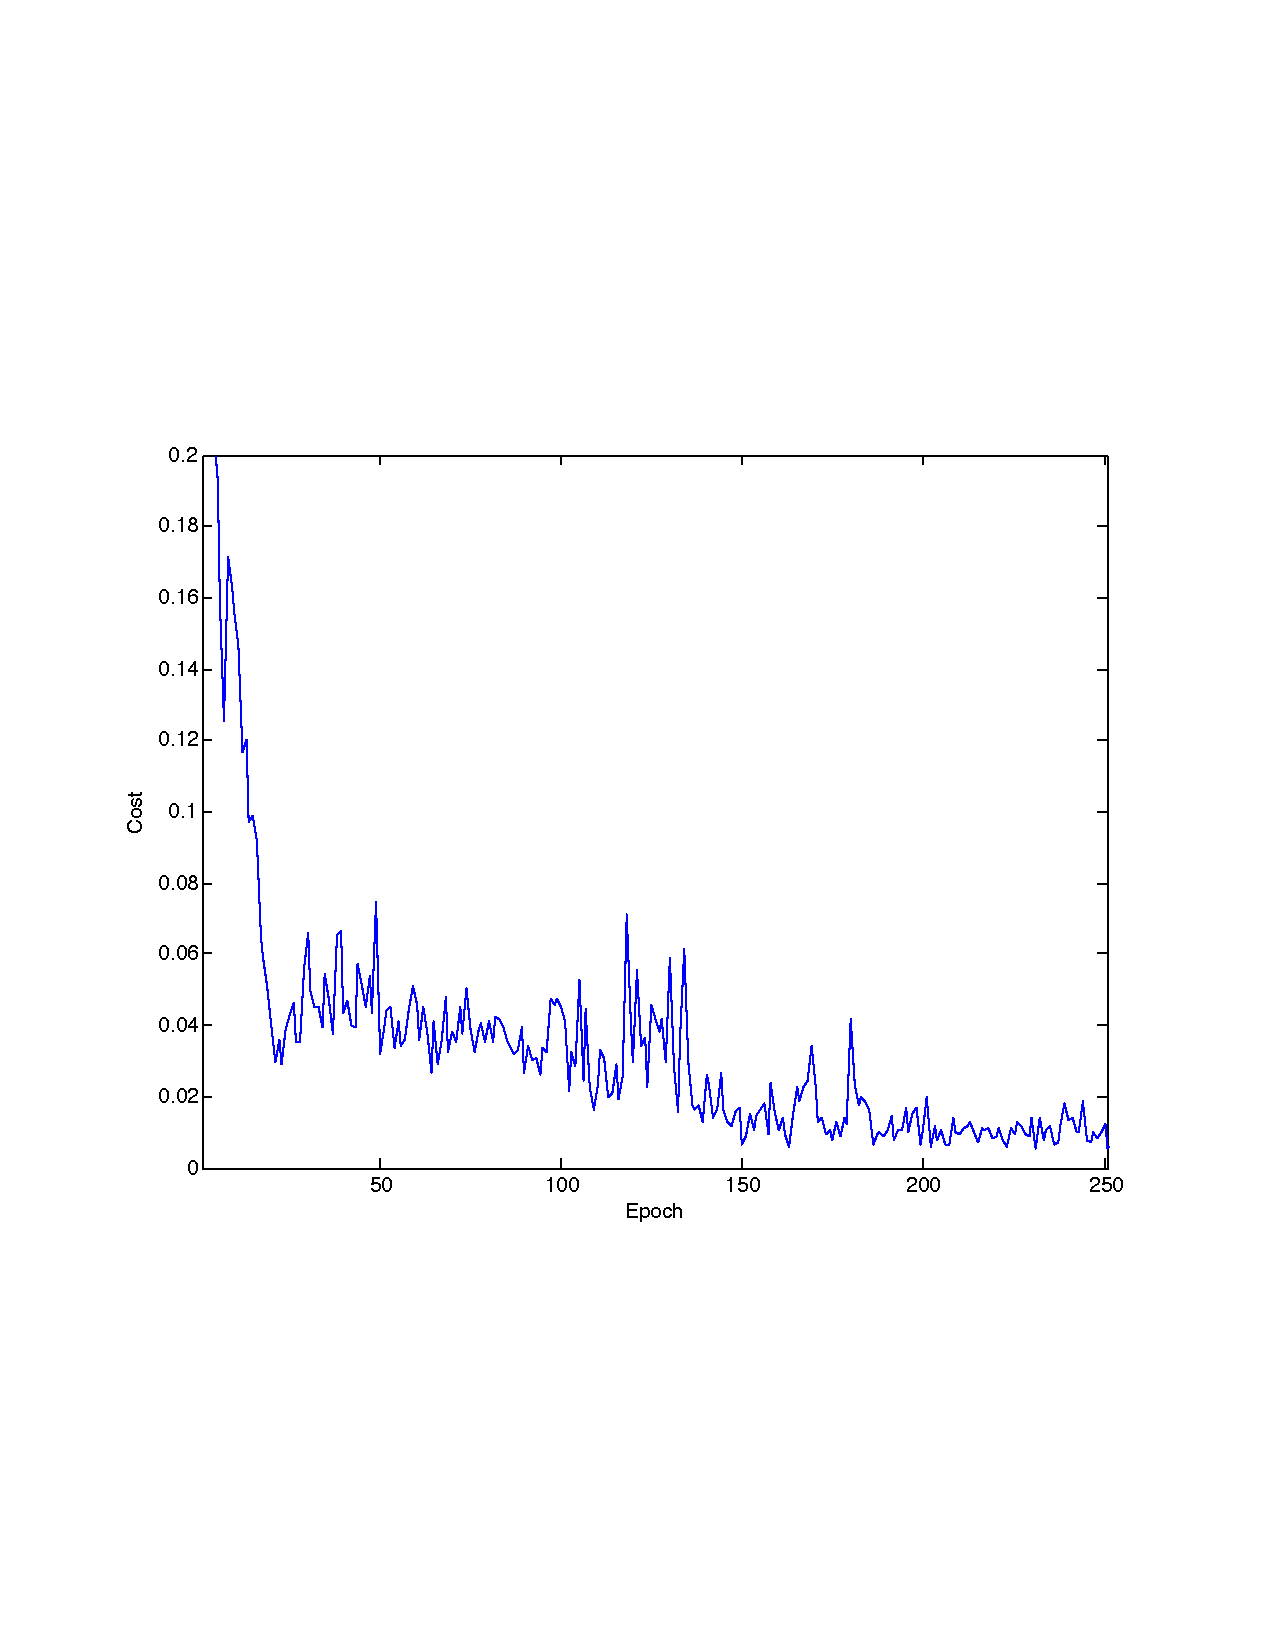
\includegraphics[width=0.5\textwidth]{Figures/sgd.pdf}}
\end{tabular}
\caption{A simple example of a neural network fitting an absolute value function (A) and the corresponding learning curve for stochastic gradient descent (B). Generated with \texttt{mlpDemo.m}.}
\label{fig:universalapproximater}
\end{figure}

\subsection{Convolutional Neural Networks}

\subsubsection{Images Masks}

In the field of image analysis, the mask (or filter, or kernel) is an important construct. A \emph{convolution} is an operation involving an initial image and the mask. The operation is equivalent to flipping the mask both vertically and horizontally and then visually placing the it over each pixel in turn. The output is the sum over a pixel-wise product of the mask and the sub-image. Masks are usually symmetric, so flipping is unnecessary.

\subsubsection{Convolutional Neural Networks}

Convolutional Neural Networks (CNNs) are the current state-of-the-art in the many computer vision tasks. Their great success in image classification\footnote{See ImageNet Large Scale Visual Recognition Competition (LSVRC), 2012 (\cite{krizhevsky2012imagenet}).} heralded a resurgence of interest in neural networks and deep learning. CNNs make the specific assumption of image inputs and emulate the process of feature extraction using image masks. It has been found that using a pre-trained CNN as a general-purpose feature extractor for a simple linear model can yield significant improvements over even the most meticulously hand-crafted feature engineering (\cite{sharif2014cnn}). Another possibility is to use the pre-trained weights as an initialisation for training on a new dataset. Both are examples of transfer learning.

The cornerstone of the CNN is the \emph{convolutional layer}, a hidden layer where a square grid of weights is convolved with the input, just like an image mask (now, however, the the mask is learned as part of an all-encompassing model). The output of the convolutional layer is akin to a convolved image. Next, the non-linear activation function, ReLu (REctified Linear Unit), is applied to zero-out any negative values. Next there is a \emph{pooling} layer, emulating \emph{downsampling}. Here, each group of (usually) four values (pixels) is replaced by the maximum of the four, leaving a single most intense pixel. This pooling method is known as \emph{max pooling}. This sequence of \texttt{CONV->RELU->POOL} layers may be repeated multiple times to create a deep architecture. Finally, a few fully-connected layers round off the architecture. Though it seems far more sophisticated than a MLP, it can be shown that a CNN can be represented as a classical fully-connected neural network. For example, a convolutional layer can be represented as a sparse fully-connected layer. Various techniques have been developed for training these vast models, for example momentum optimisers, weight initialisation, and \emph{dropout}\footnote{Dropout involves deactivating (setting to $0$) hidden units in fully-connected layers according to a Bernoulli probability. This is repeated for every forward-backward pass of the network, such that every training example is trained on a different sub-graph of the network.} for regularisation.

\section{Support Vector Machines}

Russian computer scientist, Vladimir Vapnik (1936-), invented the maximum-margin classifier in 1963, which later evolved into the kernelised support vector machine (SVM).

\subsection{Kernels}

Kernel functions are used to describe a similarity measure between objects. It is often convenient to work with a kernel of the data rather than the data itself. An example of this is tf-idf cosine similarity of a bag of words representation for document classification. Another example are Gaussian kernels, which give a multivariate Gaussian probability for the difference between two observations--the smaller the difference, the greater the probability. In linear models, it is possible to reformulate a model in terms of a kernel matrix $\mathbf{K} = \boldsymbol\Phi^T\boldsymbol\Phi$, where $\boldsymbol\Phi$ is some transformation of data $\mathbf{X}$ using basis function $\phi$. This is known as the \emph{kernel trick}, and it is particularly useful, for example, when we may apply a kernel such as the \emph{radial basis function} whose corresponding basis function is infinite-dimensional, without having to compute the infinite-dimensional basis function itself. Models can be \emph{kernelised} according to some reformulation, and replacing linear kernels (dot products) with another kernel function. In the case of kNN, this can be done quite readily. Kernelising ridge regression requires a reformulation trick known as the matrix inversion lemma. Support vector machines are kernelised by reformulating the problem into its dual problem, by application of the minimax theorem. The kernel trick requires a \emph{Mercer} kernel be used, that is, such that the Gram matrix be symmetric positive-definite.

\subsection{Kernelised kNN}

The $k$ nearest neighbours algorithm classifies a data point as the majority vote of the classes of the $k$ closest training data points. By default, the distance metric is Euclidean distance, $||\mathbf{x} - \mathbf{x}'||_2^2 = \mathbf{x}^T\mathbf{x} + \mathbf{x}'^T\mathbf{x}' - 2\mathbf{x}^T\mathbf{x}'$. It is therefore clear we can replace the inner products with any kernel function of our choosing.

\subsection{Matrix Inversion Lemma}

We will here derive a result that we will use below, known as the Woodbury matrix identity, or the matrix inversion lemma. Given matrices $\mathbf{X} \in \mathbb{R}^{M\times N}$ and $\mathbf{Y} \in \mathbb{R}^{N\times M}$, consider,

\begin{align}
\mathbf{X}\mathbf{Y}\mathbf{X} + \mathbf{X} &= \mathbf{X}(\mathbf{Y}\mathbf{X} + \mathbf{I}_N) \label{eq:mli1} \\
&= (\mathbf{X}\mathbf{Y} + \mathbf{I}_M)\mathbf{X} \label{eq:mli2}
\end{align}

Equating (\ref{eq:mli1}) and (\ref{eq:mli2}), and multiplying by left and right inverses,

\begin{align}
(\mathbf{X}\mathbf{Y} + \mathbf{I}_M)\mathbf{X} = \mathbf{X}(\mathbf{Y}\mathbf{X} + \mathbf{I}_N) &\implies \mathbf{X}^{-1}(\mathbf{X}\mathbf{Y} + \mathbf{I}_M)^{-1} = (\mathbf{Y}\mathbf{X} + \mathbf{I}_N)^{-1}\mathbf{X}^{-1}\notag\\
&\implies (\mathbf{X}\mathbf{Y} + \mathbf{I}_M)^{-1}\mathbf{X} =  \mathbf{X}(\mathbf{Y}\mathbf{X} + \mathbf{I}_N)^{-1},\notag
\end{align}

where the final step is achieved by multiplying both sides by $\mathbf{X}$ to the left and right.

\subsection{Reformulating Ridge Regression}

If we apply the matrix inversion lemma to the optimal parameters of a ridge regression, we obtain,

$$\boldsymbol{\beta}^* = (\mathbf{X}^T\mathbf{X} + \lambda\mathbf{I}_D)^{-1}\mathbf{X}^T\mathbf{y} = \mathbf{X}^T(\mathbf{X}\mathbf{X}^T + \lambda\mathbf{I}_N)^{-1}\mathbf{y} = \mathbf{X}^T\boldsymbol\alpha,$$

where $\boldsymbol\alpha = (\mathbf{X}\mathbf{X}^T + \lambda\mathbf{I}_N)^{-1}\mathbf{y}$ is a vector of \emph{dual} variables. This demonstrates that the optimal primal parameters $\boldsymbol\beta^*$ lie in the \emph{row} space of $\mathbf{X}$. By contrast, the output $\mathbf{y} = \mathbf{X}\boldsymbol\beta$ lies in the \emph{column} space of $\mathbf{X}$. There is a useful result called the \emph{representer theorem} which states that the primal and dual solutions are always related in this way for models of like form, that is, models with a loss function and penalty term. This is useful, as it is easier to solve the dual problem for support vector machines.

\subsection{Decision Boundaries}

Consider a simple binary classifier,

\begin{equation}
f(\mathbf{x}) = \text{sgn}\big(f(\mathbf{x})\big),
\label{eq:svmprimal}
\end{equation}

where $f(\mathbf{x}) = \mathbf{w}^T\mathbf{x} + b$, that is, returning $-1$ if $f(\mathbf{x}) < 0$ and $1$ if $f(\mathbf{x}) > 0$. The function is linear and has a linear decision boundary. It is useful to consider how the model parameters relate to the decision boundary. The decision boundary are those points $\mathbf{x}$ such that $f(\mathbf{x}) = 0$, hence on the boundary between the two classes. Consider the two-dimensional case where $f(\mathbf{x}) = w_1x_1 + w_2x_2 + b = 0$ (Figure \ref{fig:decisionboundary}A). For $\mathbf{x} = [x_1, x_2]$ on the decision boundary, consider $x_1 = 0 \implies x_2 = -b/w_2$, and $x_2 = 0 \implies x_1 = -b/w_1$. Then, the vector $\mathbf{x} = [0, -b/w_2] - [-b/w_1, 0] = [b/w_1, -b/w_2]$, runs parallel to the decision boundary. Clearly, $\mathbf{w}$ is orthogonal to $\mathbf{x}$, and this result can be shown to hold in higher dimensions also. A vector, $\mathbf{x}$, on the decision boundary and running parallel to $\mathbf{w}$, can be expressed as $\mathbf{x} = |\mathbf{x}|\cdot\mathbf{w}/|\mathbf{w}|$. Now, $f(\mathbf{x}) = \mathbf{w}^T|\mathbf{x}|\cdot\mathbf{w}/|\mathbf{w}| + b = 0$, hence $|\mathbf{x}| = -b/|\mathbf{w}|$. We thereby see that the bias term scales the distance of the decision boundary from the origin.

\begin{figure}
\centering
\begin{tabular}{cc}
\subfloat[]{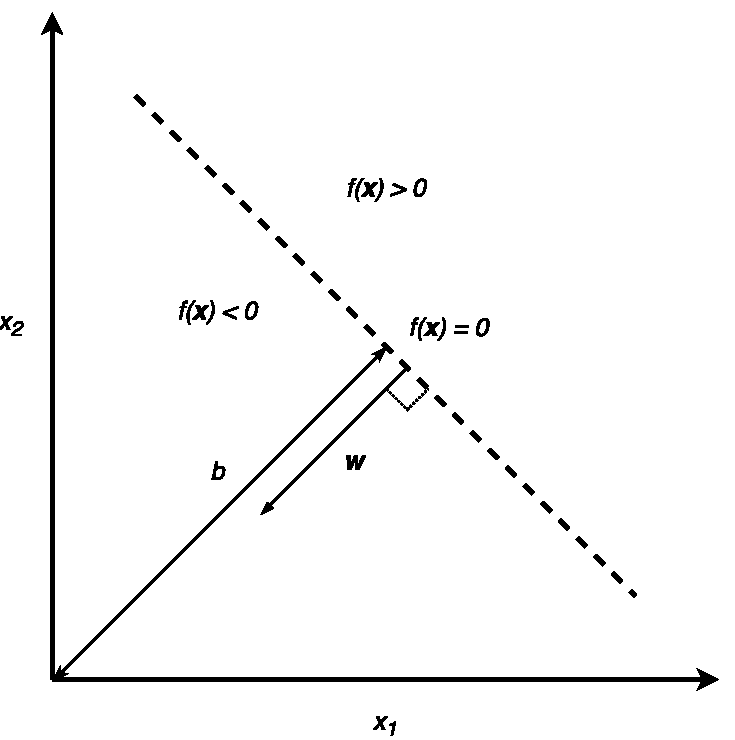
\includegraphics[width=0.49\textwidth]{Figures/decision.pdf}} & 
\subfloat[]{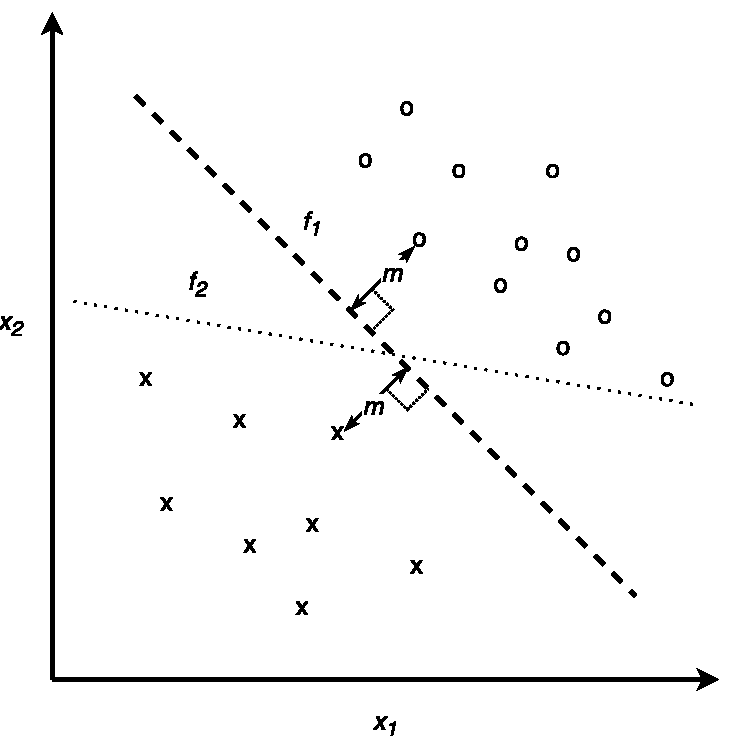
\includegraphics[width=0.5\textwidth]{Figures/maximummargin.pdf}}
\end{tabular}
\caption{The relationship between a linear decision boundary and model parameters in two dimensions (A), and comparing a maximum margin, $f_1$, with an alternative, $f_2$ (B).}
\label{fig:decisionboundary}
\end{figure}

Among the infinite possible decision boundaries we could create, a promising heuristic for separating data would be to create a decision boundary such that the perpendicular distance between the nearest data points of each class is maximised\footnote{Note that we are assuming temporarily that the data is linearly separable. This shortcoming will be addressed shortly.}. Unlike the alternatives, this maximises the \emph{space} left for unseen test cases that fall close to the boundary, likely increasing the performance of the classifier (Figure \ref{fig:decisionboundary}B). This principle is embodied in support vector machines (SVM). Therefore, SVMs are not based on statistical assumptions, rather on the rule of thumb that maximum margins perform better.

Now, any point $\mathbf{x}$ can be decomposed into the sum of its projection onto the decision boundary, $\hat{\mathbf{x}}$, and the residual, perpendicular to the boundary (and parallel to $\mathbf{w}$). Thus, $\mathbf{x} = \hat{\mathbf{x}} + r\cdot\mathbf{w}/|\mathbf{w}|$, where $r$ is the length of the residual, hence the size of the margin of $\mathbf{x}$. Thus, $f(\mathbf{x}) = \mathbf{w}(\hat{\mathbf{x}} + r\cdot\mathbf{w}/|\mathbf{w}|) + b =  |\mathbf{w}|\cdot r$, since $f(\hat{\mathbf{x}}) = 0$. Thus, we have $r = f(\mathbf{x})/|\mathbf{w}|$. Maximising the margin between the nearest points can therefore be expressed as the quadratic programming (QP) problem,

$$
\begin{array}{rl}
\min_{\mathbf{w}, b} & \frac{1}{2}\mathbf{w}^T\mathbf{w} \\
\text{subject to} & y_i(\mathbf{w}^T\mathbf{x}_i + b) \geq 1, \forall i
\end{array}
$$

where the constraints ensure each data point is correctly classified. Of course, the assumption of linear separability is in general untrue, so we introduce slack variables, $\xi_i$, to allow for data on the wrong side of the decision boundary, that is, for misclassifications. Thus, we replace each constraint with, $y_i(\mathbf{w}^T\mathbf{x}_i + b) \geq 1 - \xi_i$, leaving,

$$
\begin{array}{rl}
\min_{\boldsymbol\xi, \mathbf{w}, b} & \frac{1}{2}\mathbf{w}^T\mathbf{w} + C\sum_{i = 1}^{N}\xi_i \\
\text{subject to} & y_i(\mathbf{w}^T\mathbf{x}_i + b) \geq 1 - \xi_i, \forall i \\
& \xi_i \geq 0, \forall i
\end{array}
$$

%$$
%\begin{array}{rl}
%\min_{\boldsymbol\alpha} & \inf_{\boldsymbol\xi, \mathbf{w}, b}\bigg(\frac{1}{2}\mathbf{w}^T\mathbf{w} + C\sum_{i = 1}^{N}\xi_i + \sum_{i=1}^N \alpha_i(1 - \xi_i - y_i(\mathbf{w}^T\mathbf{x}_i + b))\bigg) \\
%\text{subject to} & \alpha_i \geq 0, \xi_i \geq 0, \forall i
%\end{array}
%$$

where $C$ is a weight for classification error. This problem is often expressed in terms of a hinge loss function, following the notation of other regression models. By the principle of convex duality, we can convert this problem into its dual form where the dual variables $\alpha_i$ are the Lagrange multipliers of the earlier constraints. The dual form is then the maximum of the \emph{infimum}\footnote{The infimum of a set is its greatest lower-bound, the counterpart of the \emph{supremum}, the least upper-bound. Some sets have these bounds without having a defined minimum or maximum. For example, the set $\{x : 0 < x < 1\}$ has no minimum or maximum, but its infimum is 0 and supremum is 1.}  of our current problem. We can find the infimum of this expression by taking derivatives of each of the parameters, thus $\frac{\partial f}{\partial \mathbf{w}} = \mathbf{w} - \sum_{i=1}^N \alpha_iy_i\mathbf{x}_i = 0 \implies \mathbf{w}^* = \sum_{i=1}^N \alpha_iy_i\mathbf{x}_i$ at optimality, which may be substituted into the objective function. For the bias term, $\frac{\partial f}{\partial b} = \sum_{i=1}^N \alpha_iy_i = 0$ at optimality. For the slack variables, 
$\frac{\partial f}{\partial\xi_i} = C - \lambda_i \implies \lambda_i \leq C$ at optimality, where the inequality arises from the positivity constraint on $\xi_i$. Thus, the parameters are eliminated by substitution, and the bias and slack variables correspond with constraints on the dual variables, giving the dual form,

\begin{equation}
\begin{array}{rl}
\max_{\boldsymbol\alpha} & \sum_{i = 1}^{N}\alpha_i + \frac{1}{2}\sum_{i}^N\sum_{j}^N \alpha_i\alpha_jy_iy_j\mathbf{x}_i^T\mathbf{x}_j \\
\text{subject to} & \sum_{i=1}^N \alpha_iy_i = 0 \\
& 0 \leq \alpha_i \leq C, \forall i
\end{array}
\label{eq:dual}
\end{equation}

thus a quadratic programming (QP) problem in the dual variables. Noting the relation between primal and dual parameters, we can rewrite the classifier (\ref{eq:svmprimal}) in terms of the dual variables as,

\begin{equation}
f(\mathbf{x}) = \text{sgn}\Bigg(\sum_{i=1}^N \alpha_iy_i\kappa(\mathbf{x}_i, \mathbf{x}) + b\Bigg),
\label{eq:svmdual}
\end{equation}

where $\kappa(\cdot, \cdot)$ is a Mercer kernel of our choosing, replacing the linear inner product from before. Apart from the dual form being conveniently kernelised, it affords an insightful alternative interpretation of the model. From (\ref{eq:svmdual}), we can see how an observation, $\mathbf{x}$ is classified according to its similarity with the training vectors. Each training vector, $\mathbf{x}_i$, casts its vote, $y_i$, be it $-1$ or $1$, with the influence regulated by a similarity measure provided by the kernel function, and the weight provided by the dual variable. Only the support vectors have a (non-zero) weighted vote. It is easy to see why this is such a powerful framework--we can choose between many similarity measures (kernels), though the mathematics restricts us to choosing Mercer kernels.

\subsection{Sequential Minimal Optimisation}

Our model (\ref{eq:svmdual}) may be solved with any QP solver, which was formerly the standard approach. However, in 1998, American computer scientist, John Platt (1963-), invented sequential minimal optimisation (SMO), an algorithm for analytically optimising the dual variables two at a time. The superiority and simplicity of this algorithm helped bring support vector machines into the forefront of machine learning research. The algorithm works by iteratively optimising pairs of variables that violate the optimality conditions. These are,

\begin{equation}
\begin{array}{rcl}
\alpha_i = 0 & \implies & y_if(\mathbf{x}_i) \geq 1 \\
0 < \alpha_i < C  & \implies & y_if(\mathbf{x}_i) = 1 \\
\alpha_i = C & \implies & y_if(\mathbf{x}_i) \leq 1
\end{array}
\label{eq:svmkkt}
\end{equation}

Optimisation is done in pairs in order to maintain the equality constraint of the problem (\ref{eq:dual}). Thus, for pair $\alpha_i$ and $\alpha_j$, we make updates such that $y_i\Delta\alpha_i + y_j\Delta\alpha_j = 0$. Rearranging gives $\Delta\alpha_j = -\Delta\alpha_iy^{(i)}/y^{(j)} = -\Delta\alpha_iy^{(i)}y^{(j)}$, as since $y_i \in \{-1, 1\}$, division is the same as multiplication, and the cost function becomes,

\begin{align}
W(\boldsymbol\alpha) &= \sum_{k=1}^N\alpha_k + \Delta\alpha_i -\Delta\alpha_iy_iy_j - \frac{1}{2}\sum_{k=1}^Ny_k\alpha_k(f(\mathbf{x}_k) - b) \notag \\ 
&- \Delta\alpha_i(f(\mathbf{x}_i) - f(\mathbf{x}_j)) - \Delta\alpha_iy_i(f(\mathbf{x}_i) - f(\mathbf{x}_j)) - \frac{1}{2}\Delta\alpha_i^2(\mathbf{x}_i^T\mathbf{x}_i - 2\mathbf{x}_i^T\mathbf{x}_j + \mathbf{x}_j^T\mathbf{x}_j). \notag 
\end{align}

Differentiating and solving gives,

$$\Delta\alpha_i^* = \frac{y_i\big(f(\mathbf{x}_j) - y_j - f(\mathbf{x}_i - y_i)\big)}{\mathbf{x}_i^T\mathbf{x}_i - 2\mathbf{x}_i^T\mathbf{x}_j + \mathbf{x}_j^T\mathbf{x}_j},$$

giving us our update step. The value of $\Delta\alpha_j^*$ can then be determined from the initial equality. Note that both variables remain constrained, hence their values must be clipped if they are less than $0$ or greater than $C$. The bias term is then updated to account for the changes. For example, to ensure the classifier now emits $y_i$ for $f(\mathbf{x}_i)$, we rearrange,

$$y_i = \sum_{k=1}^N \alpha_iy_i\mathbf{x}_k^T\mathbf{x}_i + b + \Delta b + \Delta\alpha y_i\mathbf{x}_i^T\mathbf{x}_i + \Delta\alpha y_j\mathbf{x}_i^T\mathbf{x}_j,$$

for $\Delta b^*$. The same is done for $f(\mathbf{x}_j)$, and the expressions are combined according to the convergence conditions (\ref{eq:svmkkt}). Thus, the optimisation steps are done analytically, rather than with linear algebra. The rest of the algorithm is mostly concerned with heuristics for choosing the best $\alpha_i$, $\alpha_j$ pair. An implementation of support vector machines solved with the SMO algorithm is given in \texttt{supportVectorMachine.m}.

\subsection{Support Vector Machine Regression}

The ideas of support vector machines can be extended to regression models as well. This is achieved using a modification of the Huber loss function, creating a constrained quadratic programming (QP) problem. One of the shortcomings of SVMs is the difficulty in extending them to multi-class classification. This stems from the fact that they are not probabilistic models. However, schemes exist, for example, by training multiple classifiers in a hierarchy.

\section{Decision Trees}

Decision trees are distinct from the previously discussed classifiers in that they are \emph{non-parametric}. This means the model is not simply a mathematical function with a fixed form, and that the size of the model changes depending on the size of the data\footnote{Non-parametric methods could be said to ``let the data do the talking''.}.

\subsection{Learning Decision Trees}

Just as with regression, we begin with a dataset, $\mathcal{D} = \{(\mathbf{x}_n, y_n)\}_{n=1}^{N}$. Now, however, the output variable, $y \in \{0, 1, \dots, K-1\}$, is a discrete variable taking a value in one of $K$ categories. For simplicity, we will consider the case that $K = 2$, that is, binary classification. We therefore search for a way of splitting the data into two groups. We repeat this procedure for each of the subgroups recursively, until we satisfy some stopping condition. In so doing, we create a binary tree. Prediction can therefore be done by tracing a data point through the splitting conditions of the tree. Note this is an example of \emph{embedded feature selection} (\cite{featureselectionsurvey}).

The only question then is \emph{how} we should split the data. For example, if we are classifying vehicles, and $y \in \{\text{car}, \text{motorbike}\}$, and our data consists of categories, $\mathbf{x} = [\text{number wheels}, \text{colour}, \text{milage}]$, the number of wheels is likely be a very effective indicator for sorting the cars from the bikes. In fact, it may be decisive, and rarely are indicators so informative in practice. The colour would likely tell us very little, but the milage might tell us something, as longer journeys are usually done by cars, so there may be a weak correlation. We therefore use an impurity measure to quantify the reduction in uncertainty upon making a given split. The best split is the one that minimises the uncertainty,

\begin{align}
( k^*, \tau^*) &= \min_{k, \tau} I_{split}(X, k, \tau) \notag \\
&= N_LI_{split}(p_L) + N_RI_{split}(p_R), \notag
\end{align}

where $L$ and $R$ denote the left and right splits of the data, $N_L$ and $N_R$ are the respective population sizes of the split data, and $p_L = \frac{\#(y = 0)}{N_L}$ and $p_R = \frac{\#(y = 0)}{N_R}$ are the sample probabilities of belonging to a given class, where in our fictitious data, $y=0$ could indicate a car, and $y=1$ a bike. Of course, when these probabilities go to 1, we are \emph{certain} of the class of the remaining data. Note the split consists of two components: the variable of split $x_k$, and the decision rule $\tau$. For example, with our fictitious data, the optimal split might be on $x_{k^*} = (\text{number wheels})$ and $\tau^* = (\text{number wheels} \leq 2)$. Clearly, this would more or less perfectly divide the bikes and the cars into distinct groups. In practice, we must systematically try all possible splits for each variable. If the variable is continuous, we must then discretise it in some way.

Several impurity measures are possible, but we know from information theory that uncertainty can be modelled with the \emph{entropy} statistic. For binary classification, we have only two probabilities, $p(y = 0)$ and $p(y=1) = 1 - p(y=0)$. We therefore have the special case of binary entropy, $h_2(p)$, and our impurity measure becomes,

$$I_{split}(p) = h_2(p) = -p\log p - (1-p)\log (1-p).$$

\subsection{More Advanced Techniques}

An extension of decision trees is the technique of \emph{random forests}. Random forests construct multiple decision trees from subsets of the training data. Prediction is then done in an \emph{ensemble} by aggregating the predictions of individual trees,

$$z(\mathbf{x}) = \frac{1}{M}\sum_{i=1}^M f_i(\mathbf{x}),$$

where the models $f_i$ are individual decision trees trained on random subsets of the data. In such a scheme they are known as \emph{weak learners}. Now, recall that,

\begin{align}
\text{Var}[X + Y] &= \mathbb{E}[(X + Y)^2] - \mathbb{E}[X + Y]^2 \notag \\
&= \mathbb{E}[X^2 + 2XY + Y^2] - \mathbb{E}{X}^2 - 2\mathbb{E}[X]\mathbb{E}[Y] - \mathbb{E}[Y]^2 \notag \\
&= \text{Var}[X] + \text{Var}[Y] + 2\text{Cov}[X, Y] \notag
\end{align}

It is easy to then show that,

$$\text{Var}\Big[\sum_i X_i\Big] = \sum_i \text{Var}[X_i] + 2\sum_i\sum_{j \neq i} \text{Cov}(X_i, X_j).$$

Consider then that in our random forest, each learner has a variance of $\sigma^2$ and $\text{Cov}(f_i, f_j) = \rho\epsilon \forall i, j, i \neq j$. Then,

$$\text{Var}\Big[\frac{1}{M}\sum_i f_i\Big] = \frac{\sigma^2}{M} + \rho\frac{M-1}{M}\sigma^2.$$

Thus, the ratio is reduced by, $M/(1 + \rho(M-1))$. We therefore aim to decorrelate the individual trees. This is done in two ways. First, the training set is sampled (with replacement) to create $M$ \emph{bootstrapped} training sets of size $N$. Used in the ensemble, this is known as \emph{bagging} (bootstrapping and aggregating). Secondly, train each learner on a random subset of the available features. The size of the subset is a model hyperparameter.

\section{Dimensionality Reduction and PCA}

The curse of dimensionality motivates techniques to transform high-dimensional data, given by an $N \times D$ matrix $\mathbf{X}$, to a lower rank approximation. This can be achieved by choosing lower dimensionality, $M  < D$, and finding $D \times M$ matrix $\mathbf{W}$ and $N \times M$ matrix $\mathbf{Z}$ such that,

$$\mathbf{X} \approx \mathbf{Z}\mathbf{W}^T,$$

and such that the \emph{reconstruction error} is minimised. This leads to the objective function,

$$\min_{\mathbf{W}, \mathbf{Z}} J(\mathbf{W}, \mathbf{Z}) = \frac{1}{N}\sum_{i=1}^N||\mathbf{x}_i - \hat{\mathbf{x}}_i||^2,$$

where $\hat{\mathbf{x}}_i = \mathbf{W}\mathbf{z}_i$ is the reconstruction of the $i$th row. The reconstruction error function can be minimised (and the optimal decomposition found) with an algorithm known as alternating least squares (ALS). It can be shown analytically that the optimal orthogonal choice occurs when $\mathbf{W}$ is the matrix of the $M$ most significant eigenvectors (highest eigenvalues) of the sample covariance matrix, $\hat{\boldsymbol\Sigma} = \frac{1}{N}\sum_i\mathbf{x}_i\mathbf{x}_i^T = \frac{1}{N}\mathbf{X}^T\mathbf{X}$. These are otherwise known as the \emph{principal components} of $\mathbf{X}$, which brings us to principal component analysis (PCA), a highly popular technique for dimensionality reduction. If we can find $\mathbf{X} \approx \mathbf{Z}\mathbf{W}^T$ for lower-dimensional, orthonormal $\mathbf{W}$, then $\mathbf{X}\mathbf{W} \approx \mathbf{Z}\mathbf{W}^T\mathbf{W} \implies \mathbf{X}\mathbf{W} \approx \mathbf{Z}$, hence $\mathbf{W}$ maps our data to a lower-dimensional approximation. When the transformation is made, a model may be trained, perhaps more successfully than with the full data.

%Note that if we take all principal components ($M = D$) and perform the transform, $\mathbf{Z} = \mathbf{X}\mathbf{W} = \mathbf{U}\mathbf{S}\mathbf{V}^T\mathbf{V} = \mathbf{U}\mathbf{S}$


The data may be decorrelated using the decomposition. Consider mapping $\mathbf{X}$ to $\mathbf{Z} = \mathbf{X}^T\mathbf{U} = \mathbf{V}\mathbf{S}\mathbf{U}^T\mathbf{U} = \mathbf{V}\mathbf{S}$. The covariance matrix for this is then, $\mathbf{Z}^T\mathbf{Z} = \mathbf{S}\mathbf{V}^T\mathbf{V}\mathbf{S} = \mathbf{S}^2$, that is, a diagonal matrix with no correlations between variables.


\subsection{Singular Value Decomposition}

Singular Value Decomposition (SVD) is a factorisation that exists for all matrices $\mathbf{X}$ written,

$$\mathbf{X} = \mathbf{U}\mathbf{S}\mathbf{V}^T,$$

where matrices $\mathbf{U}$ and $\mathbf{V}$ are orthonormal, and $\mathbf{S}$ is the diagonal matrix of \emph{singular values}. To relate SVD back to PCA, note that the empirical covariance matrix,

$$\hat{\boldsymbol\Sigma} = \mathbf{X}^T\mathbf{X} = \mathbf{V}\mathbf{S}\mathbf{U}^T\mathbf{U}\mathbf{S}\mathbf{V}^T =  \mathbf{V}\mathbf{S}^2\mathbf{V}^T,$$

which is an eigenvalue decomposition. This implies that $\mathbf{W} = \mathbf{V}$ and $\mathbf{Z} = \mathbf{X}\mathbf{W} = \mathbf{U}\mathbf{S}\mathbf{V}^T\mathbf{V} = \mathbf{U}\mathbf{S}$. The principal components are therefore the columns of the right singular matrix, $\mathbf{V}$, equivalent to the eigenmatrix of the covariance matrix. Thus, SVD (which may be done with various techniques) is an alternative to ALS for acquiring the reconstruction matrices for PCA. In this form, it is clear that a matrix multiplication can be understood in three steps: a rotation $\mathbf{U}$, a scaling $\mathbf{S}$ and a final rotation $\mathbf{V}$. For a cloud of points, $\mathbf{X}$, the principal components give the trend lines in orthogonal directions that maximise the variance. These trends can be thought of as latent variables underlying the observations and this is the essence of information retrieval techniques such as latent semantic indexing (LSI).

\section{Unsupervised Machine Learning}

Whereas supervised machine learning can be said to embody learning by example, \emph{unsupervised} machine learning is concerned with finding inherent patterns in a dataset. In this sense, its aim is \emph{description}, rather than prediction. The two most common applications of unsupervised machine learning are feature extraction and \emph{clustering}. Clustering is of particular interest to data mining applications. Clustering is the act of grouping data observations according to some grouping measure. The choice of clustering algorithm is usually problem-specific. Various approaches exist, for example density-based clustering algorithm DBSCAN (density-based spatial clustering with additive noise), or hierarchical clustering models\footnote{Hierarchical models cluster data by pairing closest data samples into groups repeatedly, creating a binary tree hierarchy in a bottom-up approach until all data belongs to a single super group. Such a clustering is usually visualised with a tree-like dendrogram.}. These techniques are popular, but are more heuristic algorithms than machine learning. The techniques we will discuss are more sophisticated and are based on fitting probability densities to data.

\subsection{K-means}

One of the most popular clustering techniques, K-means, organises data into $K$ clusters. One commonly used algorithm is closely related to (and often called by) Lloyd's algorithm for Voronoi diagrams. This efficiently gives a clustering, albeit without a guarantee on global optimality, as K-means remains NP-complete. The algorithm begins by initialising $K$ centre points in $D$-dimensional space and alternates between two steps. The first step assigns observations to centres based on a distance measure (usually Euclidean distance). Observations assigned to a common centre can then be said to be in the same cluster. For each cluster, a new centre point is calculated as the average of all observations in the cluster. This is repeated until the centre points converge (which will occur when observations cease to change clusters). Note that $K$ must be pre-selected--the algorithm does not tell us what value of $K$ is most suitable. To formalise beyond this intuitive algorithm, we denote a set of parameters, $r_{nk}$, whose binary value indicates the membership (or not) of observation $x_n$ in cluster $k$. A further set of parameters, $u_k$, denote the centre point of each of the $K$ clusters. Thus, the K-means algorithm can be formulated as the optimisation problem,

$$\min_{\mu, \mathbf{r}} \mathcal{L}(\mu, \mathbf{r}) = \sum_k\sum_n r_{nk}||\mathbf{x_n} - \mathbf{\mu}_k||^2_2,$$

where $\sum_k r_{nk} = 1$, and the distance measure is the sum of squares, $(x_n - \mu_k)^T\cdot(x_n - \mu_k)$. Now, we may write step 1:

\[r_{nk} = \begin{cases}
    1 & \text{if} \ k = \arg \min_k \ ||\mathbf{x}_n - \mu_k||_2^2 \\
    0 & \text{otherwise}
\end{cases}\]

Step 2 can then be seen as an optimisation of $\mathcal{L}$ with respect to each $u_k$. Clearly,

\begin{align}\frac{\partial\mathcal{L}}{\partial\mu_k} = \frac{\partial}{\partial\mu_k}\sum_n r_{nk} (\mathbf{x}_n^T\mathbf{x}_n - 2\mathbf{x}_n^Tu_k + u_k^Tu_k) &= 0 \notag \\
&\implies \hat{\mu}_k = \frac{\sum_nr_{nk}x_n}{\sum_nr_{nk}}, \notag
\end{align}

this is clearly the arithmetic mean of the points in the cluster. With this in mind, we may see that our loss function can be written as a maximum likelihood,

\begin{align}\min_{\mu, \mathbf{r}} \mathcal{L}(\mu, \mathbf{r}) = \max_{\mu, \mathbf{r}} \log p(\mathcal{D} | \mu, \mathbf{r}) &= \log\prod_k\prod_n \mathcal{N}(\mathbf{x}_n ; u_k, \mathbf{I})^{r_{nk}} \notag \\
&= -\sum_k\sum_nr_{nk}(\mathbf{x}_n - \mu_k)^T\mathbf{I}(\mathbf{x}_n - \mu_k), \notag
\end{align}

where $\mathbf{I}$ is the identity matrix. This shows that K-means fits $K$ Gaussian densities with unit variance. So, despite the initially simple algorithm, we see the deeper probabilistic meaning behind K-means. Because the clusters are all based on spherical Gaussians of fixed size and shape, the technique can alternatively be viewed as clustering points by nearness in Euclidean space. It is useful, however, to take note of the probabilistic notions, as these are expanded upon in the more powerful Gaussian mixture models.

\subsection{Gaussian Mixture Models}

\begin{figure}
\centering
\begin{tabular}{cc}
\subfloat[1 iteration]{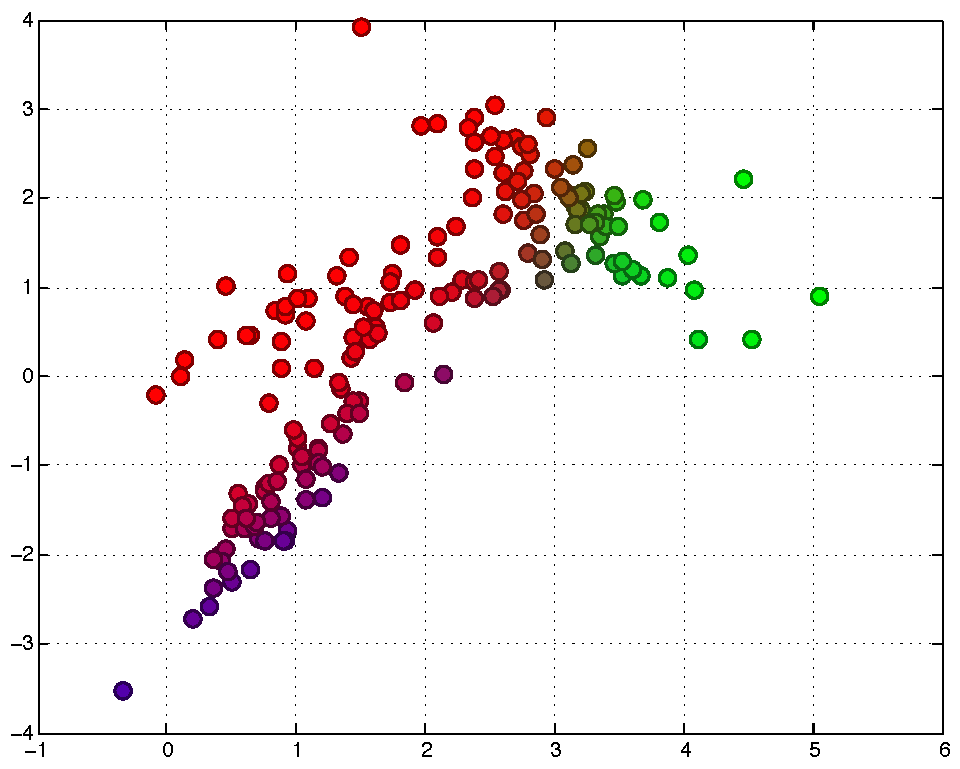
\includegraphics[width=0.5\textwidth]{Figures/gmm0.pdf}} & 
\subfloat[3 iterations]{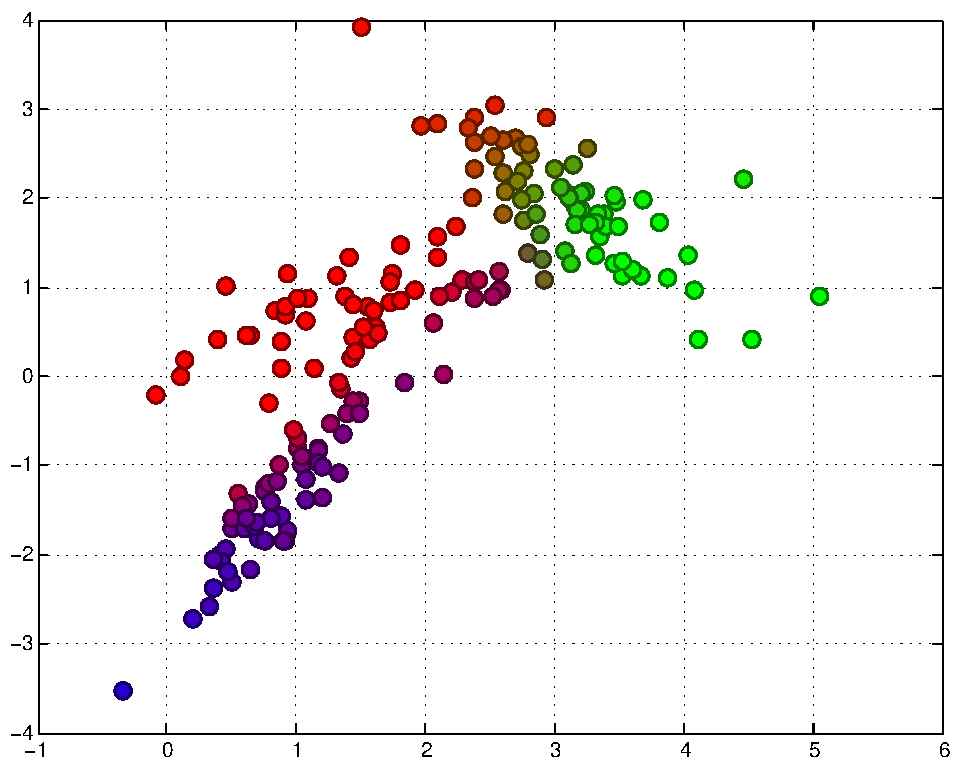
\includegraphics[width=0.5\textwidth]{Figures/gmm2.pdf}}\\
\subfloat[5 iterations]{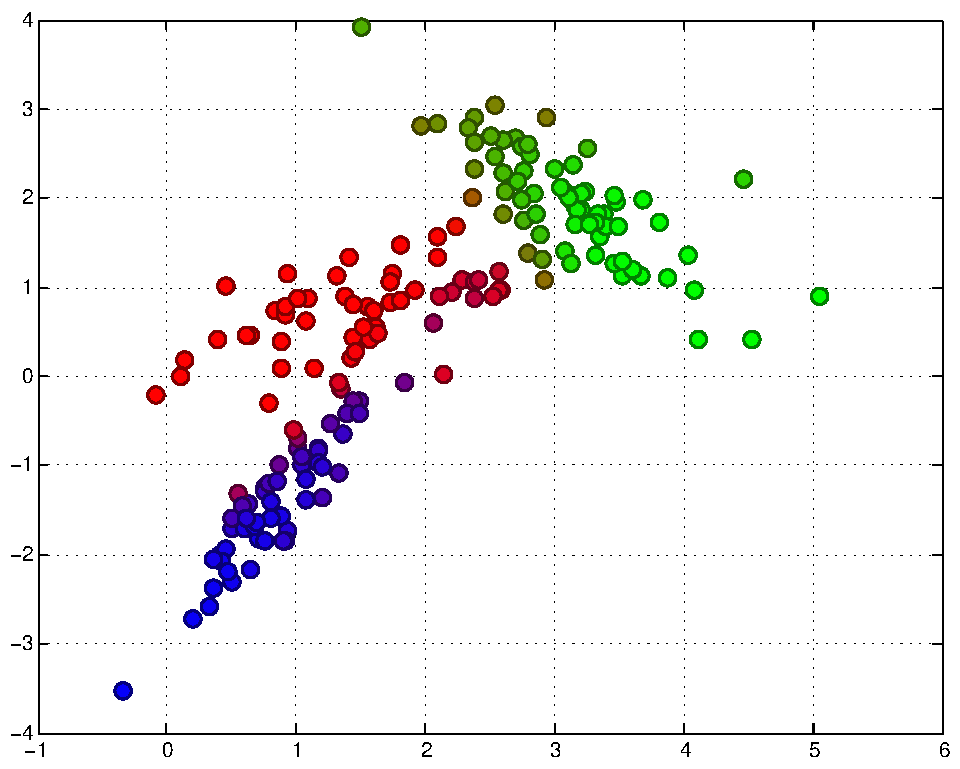
\includegraphics[width=0.5\textwidth]{Figures/gmm4.pdf}}&
\subfloat[10 iterations]{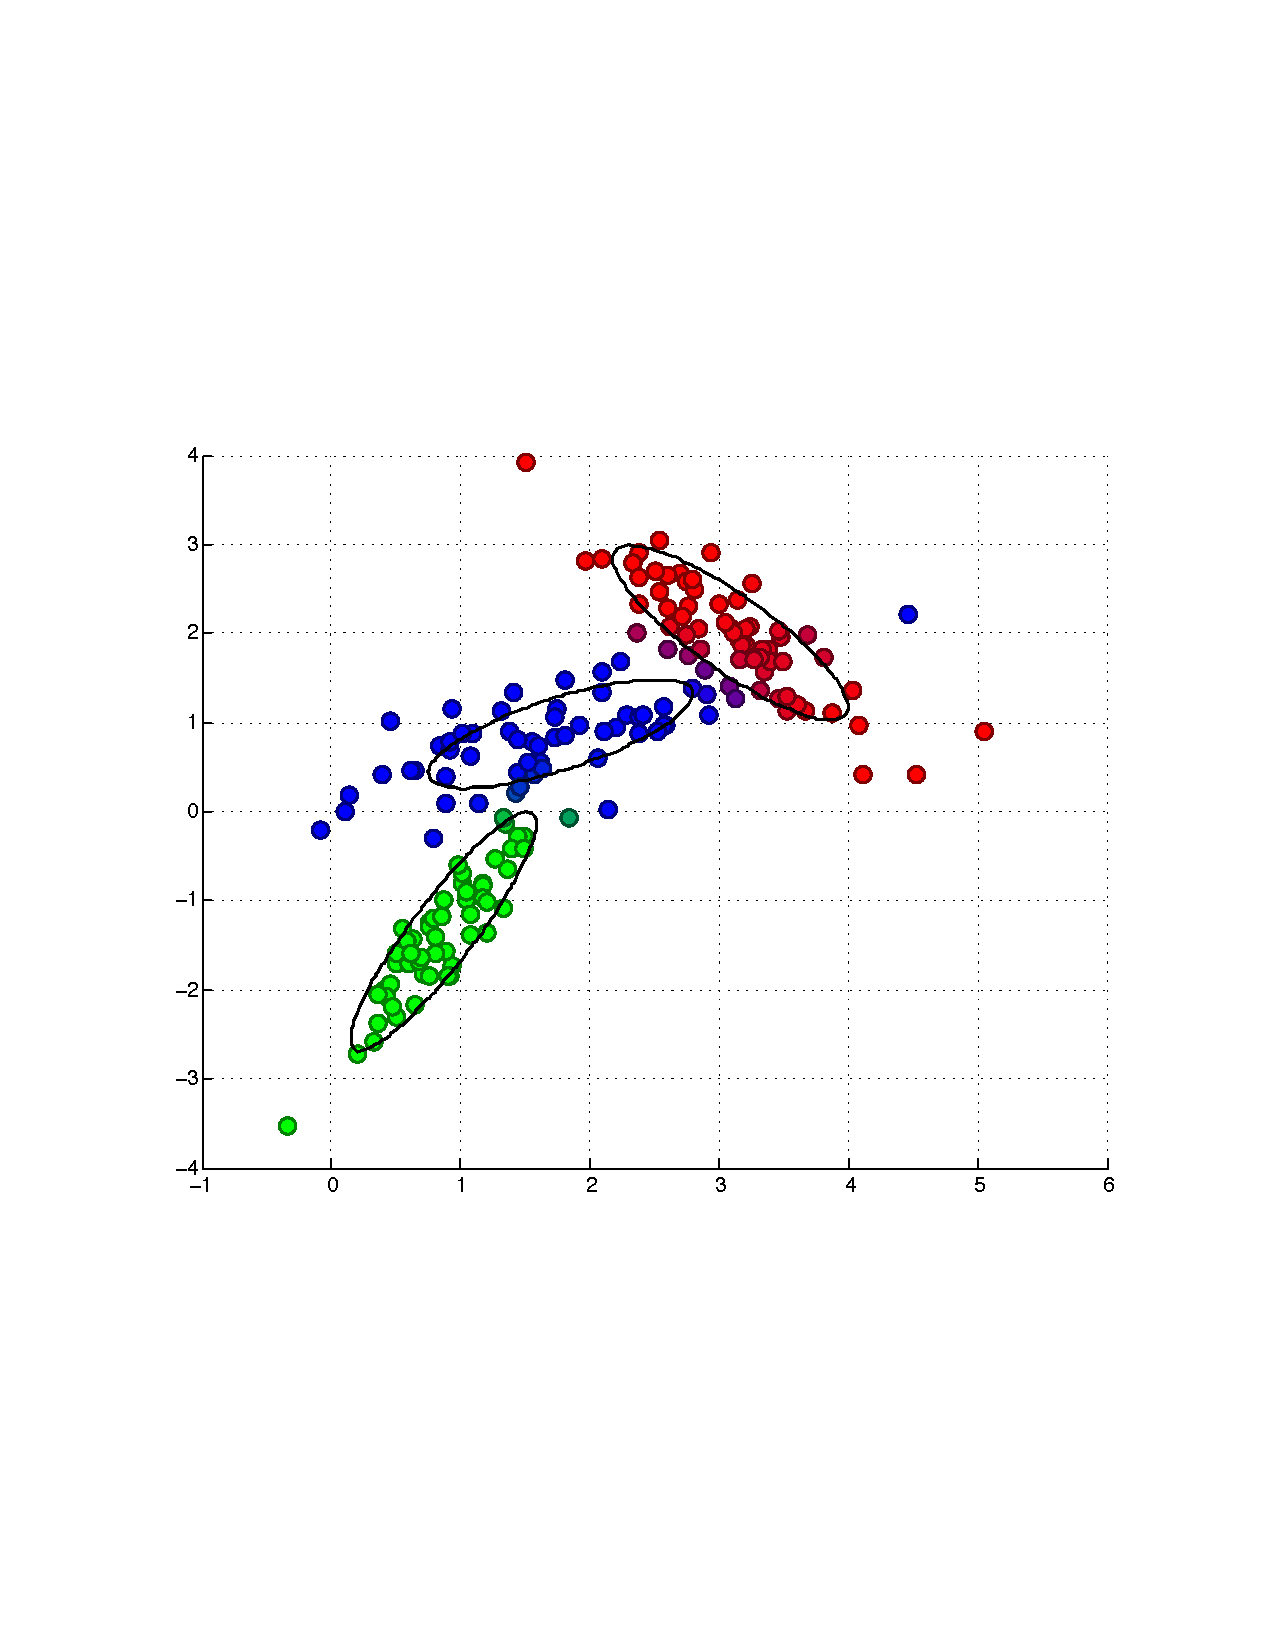
\includegraphics[width=0.5\textwidth]{Figures/gmm10.pdf}} \\
\end{tabular}
\caption{Expectation maximisation (EM) algorithm in action over 30 iterations for Gaussian mixture models with $K = 3$. Colour coding reflects the ratio of probabilities for each cluster--note that points in overlapping positions are more ambiguous. Contour plot of sample Gaussians given in final iteration. Created with \texttt{gmmDemo.m}.}
\label{fig:gmm}
\end{figure}

A more powerful clustering technique, Gaussian mixture models (GMM) improve on two major shortcomings of K-means. Firstly, GMMs fit elliptical Gaussian densities, optimising over the choice of $\boldsymbol\Sigma$, the covariance matrix. Secondly, the parameters, $r_{nk}$, are replaced by random variables, $r_n$, of a special kind called \emph{latent} random variables. These act as a bridge between each observation $\mathbf{x}_n$ (also a random variable), and its class, $k$. Thus, rather than hard binary values, the values $r_{nk} = p(r_n = k)$ indicate the probabilities of $\mathbf{x_n}$ belonging to cluster $k$. This is useful both for the fact that the parameters no longer grow with the size of the data, and also to quantify an uncertainty about $\mathbf{x}_n$, which can be used for analysis of outliers, and for example the selection of $K$. However, the complexity of the algorithm is far greater than K-means. Again, problem-specific considerations must be made when choosing the most suitable algorithm. Note that unlike spatial clustering algorithm DBSCAN, GMMs are capable of clustering densities that overlap, but are less useful when the data is not linearly separable. Thus, GMMs are good at clustering populations that are likely to be normally distributed in their features, but not, for example, geospatial data that exhibit irregular shapes. The likelihood function for GMMs is maximised using an iterative algorithm called expectation maximisation (EM) (Figure \ref{fig:gmm}), which, similar to K-means, consists of two alternating steps, the $E$ and $M$ steps. In general this is,

$$\arg \max_\theta \mathbb{E}_{p(z_n)}[\log p(x_n, r_n | \theta)].$$

\section{Performance Metrics}

Accuracy is defined to be,

$$
\text{Accuracy} = \frac{TP + TN}{TP + FN + FP + TN},
$$

that is, the proportion of correct classifications to total classifications, where TP is the number of \emph{true positives}, the number of times a class is correctly predicted to have occurred; TN is the number of \emph{true negatives}, the number of times a given class is correctly predicted not to have occurred; FN is the number of \emph{false negatives}, the number of times a class is incorrectly predicted to have occurred; and FN is the number of \emph{false negatives}, the number of times a class is incorrectly predicted not to have occurred. Accuracy can be a misleading statistic when we have uneven representations of classes in the dataset. In the event that we have a sufficiently high bias, we can achieve excellent accuracy simply by always predicting the dominant class. For this reason, we consider other statistics too. \emph{Precision} is the number of times a class is \emph{correctly} predicted proportional to the overall number of predictions for that class, that is,

$$
\text{Precision} = \frac{TP}{TP + FP}.
$$

This, however, does not inform us as to whether we have missed any occurrences of the class, which would be shown in the number of false negatives, FN. We could therefore have a very high precision with limited accuracy. \emph{Recall} is the number of times a class is \emph{correctly} predicted proportional to the number of occurrences of that class (equivalently, the accuracy with respect to the class), that is,

$$
\text{Recall} = \frac{TP}{TP + FN}.
$$

However, a simple strategy of always predicting one class will give perfect recall for that class, because then misclassifications are only captured by $FP$. The $F_1$ statistic is a common measure used to assess classifiers that combines precision and recall, and is defined as,

$$
F_1 = \frac{2 \times \text{precision} \times \text{recall}}{\text{precision} + \text{recall}},
$$

that is, the harmonic mean of precision and recall (the ``1'' in $F_1$ indicates the two are evenly weighted). The $F_1$ statistic is a neat way of summarising both metrics at once. Furthermore, a large imbalance in precision and recall results in a lower $F_1$ score. It is necessary to be good in both precision and recall to have a good $F_1$ score; the harmonic mean of any data is always upper-bounded by its arithmetic mean. Thus, the $F_1$ score addresses their shortcomings simultaneously.

\subsection{ROC Curves}

Receiver Operator Characteristic (ROC) curves are a way of assessing the performance of a binary classifier, usually visualised graphically. A ROC curve compares the true positive and false positive rates of a binary classifier over a range of thresholding choices. In practice, a classifier's predictions are output as a set of real probabilities (taking care not to round early). Points on the ROC curve are generated by calculating the resultant TP and FP rates\footnote{Note that some authors prefer to refer to the true positive rate as \emph{sensitivity} and the false positive rate as the complement of \emph{specificity}. Specificity is in fact equivalent to the \emph{true negative} rate, and is therefore complement to the false positive rate. For this reason, when these alternative terms are used, the specificity axis runs backwards on the ROC graph.} as the classification threshold is varied from 0 to 1. To illustrate, consider a low threshold: a good classifier will tend be more sure about its negatives, avoiding false negatives, even at lower thresholds. This will place the curve high on the top left corner of the graph. Over the spectrum of thresholds, a good classifier will maintain the ROC curve high above the FP-axis. The area under the ROC curve (AUROC) $\in [0, 1]$ is therefore a good indicator of the strength of a binary classifier. Further note that because \emph{rates} are used rather than absolute positives and negatives, ROC curves address the same shortcoming the accuracy measure has for unbalanced data sets.

\section{Computer Architecture}

The von Neumann architecture, named after Hungarian polymath John von Neumann (1903-1957), is the basic template for assembling a computer. It centres around a central processing unit (CPU) and primary memory source. Input and output devices may be connected to this processing core. In a modern personal computer, the components are organised across a printed circuit board (PCB)\footnote{A printed circuit board (PCB) is a plate of layered material. The top layer is made of a conductive copper and sits atop a non-conductive fibreglass layer. The circuit pattern is created by pressing a mask of the printed design to the copper plate and soaking it in an acid solution to remove the surrounding copper. Finally, a solder mask in the familiar blue or green material is placed on top of the copper traces to protect them from dust and debris, while leaving holes at the connection points. Components may then be connected to the copper circuit using melted solder (a lead-tin alloy) to fuse components to the exposed connection points. Thus, the PCB replaces traditional wiring with the copper traces, functioning as the circuitry as well as a base to which integrated circuits and other components are attached.}, known as a \emph{motherboard}. A chip is a standalone circuit with a specific function, such as memory or processing. These components are soldered onto the motherboard to connect them to the rest of the computer hardware. The wiring groups between components are known as \emph{buses}, and are used to transfer information throughout the system. However fine the motherboard circuitry is, the internal circuitry of an integrated circuit is far finer, having of the order of billions of transistors per square centimetre. When a processor is contained in a single integrated circuit, it is referred to as a \emph{microprocessor}. This is the defining characteristic of a microcomputer or personal computer (PC). Personal computers have long supplanted the large, mainframe computers of earlier decades.

The distinction between hardware and software is at times not well defined. Thus, it is difficult to talk about one without the other. Ultimately, everything exists in the physical layer, software just being structured (low entropy) configurations of electrical signals buried in the hardware. Software has varying levels of abstraction, right up to the user-friendly graphical interfaces, but at least in some sense, this is all just an illusion created by organising lower-level parts.

\subsection{Hardware}

As it is in the von Neumann architecture, the centrepiece of computer activity is the interaction between the central processing unit (CPU) and the (primary) memory--all other components are arguably peripheral to this. When a computer is turned on, a component within the CPU begins to oscillate. This is like the heartbeat of the computer, and provides a periodic \emph{clock} bit to each computation. In a Turing machine, the clock would be the invisible force driving the transitions along the tape. With some additional circuitry, the clock signal is accelerated to a \emph{clock rate} of the order of billions of hertz (Hz). This largely determines the speed of the computer, though the practical rate of computation, or floating point operations per second (FLOPS), will depend on other things, such as the efficiency of the circuitry.

The CPU first runs a primitive piece of firmware that solves the bootstrap problem\footnote{The bootstrap is conceptually the necessary prime mover for all further software on the system.}. On a PC, this is called the BIOS (Basic Input Output Software), and UEFI (Unified Extensible Firmware Interface) on a Mac. The BIOS performs checks to ensure all the hardware is functional. It also provides a user interface for making low-level changes to the system\footnote{For example, a CPU can be \emph{overclocked} to increase performance. This can be controlled from the BIOS. As a general rule, the more active the CPU is, the more voltage in its circuits per unit time. More voltage creates more heat, and thermal sensors in the motherboard cause the fans to work harder to cool the chip. Overclocking can have detrimental effects if the circuitry gets too hot.}. The BIOS is usually located on a special chip of read-only memory (ROM), installed by the manufacturer. The BIOS finds the boot loader stored in secondary memory--typically a hard disk drive (HDD) or solid-state drive (SSD), but other secondary memory such as a USB drive, CD-ROM, or the former floppy disk, are sometimes used\footnote{A user can usually interrupt the BIOS and choose where to boot from.}. The boot loader is then loaded into memory. Its task is to load the operating system (OS) into memory in turn. Again, the user may interrupt this procedure in order to choose between operating systems installed on the drive. Once the operating system is in memory it has control of the system, giving the user the ability to control the computer and load and execute other software.

\subsection{Software}

Software exists in memory as a sequence of precompiled instructions, usually loaded from secondary memory. The control unit (CU) within the CPU is hardwired to take each instruction in turn and run it through the arithmetic/logic unit (ALU) circuitry. \emph{Registers} are small, localised pieces of memory for storing inputs for CPU operations. At this level, the code is not interpreted, but rather hardwired. Each instruction has an operator code which channels execution to the appropriate circuit. The form of the instructions are defined in an assembly language, which reflects the hardwired functions provided by the processor. An example of this is the x86 and x64 Intel resp. 32-bit and 64-bit instruction sets. Assembly code is usually automatically generated from high-level language code by a compiler. The assembly code is then transformed into a binary encoding called machine code. There is more or less a one-to-one mapping between assembly and machine code. In this way, machine code is more of an encoding than a language. As an example, take the simple high-level operation \texttt{a + b}, as it would be in \texttt{C}, or another programming language. When translated to assembly code, this will look something like Algorithm \ref{alg:assembly}.

\begin{algorithm}
\caption{Assembly pseudocode for a \texttt{a + b} operation.}\label{alg:assembly}
\begin{algorithmic}[1]
\State LDR R1 a // load of 1 with variable a
\State LDR R2 b // load register 2 with variable b
\State ADD R1, R2, R3 // add register 1 and 2 and put the answer in register 3
\end{algorithmic}
\end{algorithm}

This follows what is called \emph{reverse Polish notation} (RPN), a convenient way to encode such instructions. This might then be translated to machine code as \texttt{01001100 00000010 00000011 00000100}, that is, perform operation 76 (addition) on registers 1 and 2 and put answer in register 3. Binary code is directly translatable to a system of high and low voltages. Thus, the program can exist in secondary storage as a series of electrical signals, ready to be loaded into memory by the operating system instructions for processing. To better understand how this processing works, it is necessary to descend to the electronics level.

\subsection{Digital Circuitry}

The fundamental component of electrical computers is the transistor. Conceptualised in 1926 by Hungarian physicist, Julius Edgar Lilienfeld (1882-1963), it was first implemented by a trio of Bell labs researchers in 1947, work for which they received the Nobel prize in Physics in 1956. A transistor is made of semiconductor material such as silicon (Si). It functions as a bridge between a source and sink wire, providing a third, base wire that controls the conductivity of the silicon material. If current is passed through the base wire, the bridge is opened and current flows from source to sink. In this way, the current on the main wire can be switched on or off very quickly and with no moving parts. The size of a computer overall therefore depends crucially on how small we can make transistors. Moore's law\footnote{Named after Gordon Moore (1929-), one of the founders of Intel Corporation.} predicts that the number of transistors per integrated circuit doubles every two years. This allows for building computers that are twice as powerful while retaining the same approximate size, cost, and power consumption. However, we are rapidly approaching the physical limit on transistor size. At $1.4 \times 10^{-10}\text{m}$, quantum effects are starting to interfere with accuracy.

\subsubsection{Logic Gates}

Using combinations of transistors, we can create logic gates. As it is in boolean normal forms, the only gates we need are conjunction (\texttt{AND}), disjunction (\texttt{OR}), and negation (\texttt{NOT}), and we can wire any logical circuit. An \texttt{AND} gate can be created by placing two transistors in sequence. If both transistors are activated, current will flow overall. If either or both transistors are not activated, current will not flow. Thus, it may be seen that submitting some combination of on/off (\texttt{TRUE}/\texttt{FALSE}) currents to the transistors will result in an overall on/off current through the wire, in accordance with the truth table of a logical \texttt{AND} operator. Thus, we have a circuit capable of computing a logical \texttt{AND}. An \texttt{OR} gate may be created by placing two transistors in \emph{parallel}, and a \texttt{NOT} gate or \emph{inverter} by combining positive and negative transistors.

\subsubsection{Adders}

From logic gates we can construct adders. The exclusive-or (\texttt{XOR}) operation handles the first part of binary addition: $0 \oplus 0 = 1 \oplus 1 = 0$ and $1 \oplus 0 = 0 \oplus 1 = 1$. The only thing that is not accounted for is the \emph{carry bit}. For this reason, \texttt{XOR} is called a \emph{half-adder}. It can be created in a number of ways, for example, as \texttt{OR AND NOT AND}. To create a \emph{full-adder}, it is combined with an \texttt{AND} gate to represent the carry bit. To add an 8-bit number, eight full-adders can be arranged in sequence, with each carry bit feeding into the next. More complex operations such as multiplication can be created by combining multiple full-adders. Examples of other CPU operations are the \texttt{COMPARE} and \texttt{JUMPIF} instructions. These are used in sequence to dynamically move among instructions in memory based on some logical test. This is what enables loops and if statements to occur.

\subsubsection{Memory}

The type of memory usually used as primary memory is \emph{random access memory} (RAM). Random access refers to the fact that any memory address can be accessed equally quickly. This is in contrast to a hard disk drive used for \emph{secondary} memory, where a latency of a few milliseconds is incurred to move the requested memory sector under the drive's read-write head. Increased affordability has brought about the advent of the much faster \emph{solid state}\footnote{That is, no moving parts.} (SSD) secondary memory. Note that SSD memory is still orders of magnitude slower than RAM. Despite being fast, RAM is \emph{volatile}. Volatility is a property referring to the loss of memory when the power is switched off. This contrasts with the \emph{persistent} memory provided by secondary memory sources. There are two main types of RAM: static RAM (SRAM) and dynamic RAM (DRAM). Usually SRAM is used in a CPU cache. A cache is used to store recently used data in fast memory near to the CPU. This is an heuristic strategy that helps to minimise the delay incurred on frequently used data by the much slower main memory access, the CPU being far faster. Typically, only a small cache is sufficient to speed up processing dramatically. Like logic gates, a unit of static RAM is constructed by wiring transistors in a special way. We start by wiring two \texttt{NOR} gates together such that one of the inputs of each is the output of the other. The remaining input wires are denoted the \emph{set} and \emph{reset} wires. With this configuration, it is possible to send current through the set and reset wires to switch the signals between the \texttt{NOR} gates, and such that this signal persists when the current stops. This mechanism is called a RS latch, and provides a way to store a binary signal. When combined with a wire for write data, and the CPU clock bit, we can create what is called a \emph{flip-flop}. Each flip-flop is used to store a single bit of information, and these are arranged into an array that can be addressed by row and column number. In contrast, DRAM is cheaper and more suited to primary memory storage. This consists of an array of capacitors to store bits. The capacitors only hold the bit signal for a small amount of time (milliseconds), so a mechanism is used to quickly read and rewrite memory periodically (every 100 nanoseconds or so). This is why DRAM is known as \emph{dynamic}, though it might better be referred to as \emph{extra-volatile} memory.

\subsection{Operating Systems}

An operating system (OS) is the primary software running on a computer. As well as generally providing the user with a means of manipulating the computer, it facilitates the running of other programs on the hardware. A program is loaded into memory as a \emph{process}, with its own \emph{heap} of memory. A heap is a contiguous block of main memory. When memory is allocated dynamically in a language like \texttt{C} it takes it from the process heap. Segmentation faults occur when memory on the heap is abused. A process consists of one or more \emph{threads}, which represent streams of execution. Each thread has a \emph{stack}, which is a FIFO queue for instructions and data. The stack is pushed and popped in accordance with the requirements of the program. The stack grows with the initialisation of local variables, but also with each new call to a nested function. Therefore, a maximum recursion depth is imposed by many languages to prevent the stack memory allowance being exceeded, an event known as a \emph{stack overflow}. A process scheduler in the operating system controls the access to hardware resources for each process. This is essential to a multiprogramming operating system. Input and output devices are connected to the bus with addresses. IN/OUT instructions can send or retrieve data from these devices via a data bus. The operating system provides \emph{driver} software for interfacing with hardware components. The heart of an operating system is the kernel. This provides various services for memory allocation of processes, organisation of the OS file system, handling interrupts from peripheral devices, and so on.

\subsubsection{The Unix Story}

Unix is an important operating system that was developed at Bell Labs by American computer scientists Ken Thompson (1943-) and Dennis Ritchie (1941-2011). It is the ancestor of many of the most widely used operating systems used today. At the time, Unix was favoured due to its speed, stability, modularity, and security. Unix was the first operating system written in a high-level language (\texttt{C}, itself created by the same people), and was thus portable to any hardware with a \texttt{C} compiler. It also had just the right set of innovations to make it the ideal operating system, for example \emph{piping}, used to chain software together via their outputs. However, Unix was proprietary software owned by AT\&T\footnote{Bell Labs, NJ, was owned by AT\&T for most of the 20th century. It is credited with inventing radio astronomy, the transistor, information theory, \texttt{C}, \texttt{C++}, Unix, and the one time pad (Vernam cipher). It is now owned by Nokia.}, and interest developed to create free equivalents. In particular, MIT AI lab programmer Richard Matthew Stallman (1953-), started the Free Software Foundation (FSF) and the GNU (GNU's Not Unix!) project to create a free operating system. This was a pioneering initiative in the history of open-source software.

Apart from being free to use, the idea of a GNU operating system was to expand \emph{user land}, that is, the part of the OS flexible to a user's preferences, having only a ``micro-kernel'' and a set of replaceable daemons\footnote{In Unix, daemons are named with a trailing `d'. This is why the Apache HTTP Server, \texttt{httpd}, (the most commonly used web server) is so named.}. The sense of \emph{free} software is really to do with free control over the software--gratuity is only one part of that. The GNU micro-kernel is in contrast to a complete, \emph{monolithic} kernel such as the Linux kernel. The micro-kernel was to be known as Hurd (a gnu is a type of antelope). Due to some technical difficulties, progress stalled and the project was supplanted by the Linux project, developed by Finnish programmer, Linus Torvalds (1969-), taking with it much of the support and enthusiasm for GNU. Later, divisions arose in the GNU community due to the divisive political vision of GNU. The GNU project did, however, create a large amount of very important software, for example the GNU compiler collection (GCC), the GNU Core Utilities (reimplementations of \texttt{cat}, \texttt{ls}, \texttt{rm}, etc.) the BASH shell\footnote{The Bourne Again Shell was an open-source replacement for the Unix Bourne Shell, an improvement to the Thompson Shell (no scripting).}, \texttt{glibc} (GNU's implementation of the C standard library), the GNOME desktop environment (which runs on the X Windows system for bitmap displays), and Emacs. These tools are used on many other operating systems, including Windows, OS X, and Linux. It is for this reason that Richard Stallman refers to Linux as a \emph{GNU} operating system with Linux kernel. It is unclear whether the pure GNU operating system will ever be finished, but its legacy endures. Another notable output of the movement was the GNU Public License (GPL), a software license supporting \emph{copyleft} practices, that is, free reuse of intellectual property, provided the same copyleft open-source license is retained, and therefore the ability to reuse that software too. Such an arrangement can be described as \emph{share-alike}, and is adopted by other open source licenses\footnote{There are more permissive licenses such as Berkeley Software Distribution (BSD) and the MIT license, arguably even more permissive than BSD. This comes only with the disclaimer that the author shall not be responsible for adverse effects caused by the free use of their software. The GNU Lesser General Public License (LGPL) was created as a compromise between MIT/BSD and GNU GPL. Note also that these licenses are free to use, the copyright is applied without the need to register the software. The license text is usually put in a project file marked \texttt{LICENSE}. In short, GPL is a copyleft license, BSD is an acknowledgement, and MIT is a disclaimer.}.

At approximately the same time, the systems lab at the University of California, Berkeley, were extending their licensed version of Unix, in particular, extending its TCP/IP functionalities. This came to be known as the Berkeley Software Distribution (BSD) of Unix, but it remained subject to AT\&T licensing restrictions. The Unix parts were gradually rewritten, and BSD and its variants (FreeBSD, OpenBSD, and others) came under the BSD license, a highly permissive license, allowing the full reuse of software, even in proprietary products, provided inclusion of the license text. Many of the operating systems of the present day are descended from Unix via the free alternatives of BSD. For example, BSD forms a large part of Apple's OS X operating system. BSD was the subject of a law suit by the Unix proprietors in the early 90s, during a time nicknamed the ``Unix wars'', with BSD ultimately winning the case. Unlike Linux, BSD does not use GNU, it has its own OS software including, for example, the famous vi editor. Linux is more user-friendly, however, with BSD having a command line interface (CLI) orientation. Thus, whereas GNU reverse engineered Unix, BSD evolved from it directly like the ship of Theseus. Both extended it far beyond its initial capabilities. Because of them, we now have whole families of software that are deemed ``Unix-like''.

\section{Useless Maths Facts}

\begin{itemize}
\item The length : width ratio of all standard paper sizes (A4, A5, etc.) is $\sqrt{2}:1$. It is easy to show folding a sheet of paper in half width-ways retains this same ratio. 
\item There are $10!$ seconds in 6 weeks
\item Mersenne primes are primes of the form $2^n - 1$ for some integer $n$. The Great Internet Mersenne Prime Search (GIMPS) is an ongoing collaborative experiment to find Mersenne primes. The largest Mersenne prime (and largest known prime) found to date is $2^{74207281} - 1$. Only 49 Mersenne primes have ever been found.
\item $1/e \approx 37\%$
\item Pairs of primes of difference two (e.g. 5, 7) are known as twin primes. Pairs of primes of difference four (e.g. 7, 11) are known as cousin primes. Pairs of primes of difference six (e.g. 11, 17) are known as sexy primes.
\item According to legend, the Pythagorean mathematician, Hippasus, was killed for proving the existence of irrational numbers. This conflicted with the dogmatic worldview of the other Pythagoreans.
\item For any map (for example, one of a geographic region), there is always a way to colour the map with at most four colours such that no two sections of the map sharing a border have the same colour. This comes from the four colour theorem, the first theorem in the world to be proved (partially) by computer (brute force).
\item The mirror reflection of 3.14 closely resembles the word `pie'.
\item Perfect numbers are those whose factors (including 1) sum to itself. For example, $6 = 1 + 2 + 3$. Amicable numbers are pairs of numbers each of whose factors sum to the other. For example 220 and 284.
\item 23 is the first number at which the Birthday paradox gives a greater than $50\%$ chance of a collision
\item $2^{20} \approx 10^6$
\item One googol is $10^{100}$, that is, 1 followed by 100 zeroes. A googolplex is $10^{\text{googol}} = 10^{10^{100}}$. A \emph{googolplexian} is $10^{\text{googolplex}} = 10^{10^{10^{100}}}$.
\item Graham's number is a famous named number larger by incomprehensible magnitudes. It provides an upper bound to the solution of a problem in graph theory. It is so large, it can only practically be written in terms of amalgamations of hyper-operations, exponentiation being absurdly insufficient. Using the specialised Knuth's arrow notation, Graham's number can be written as the last in a sequence 64 numbers, the first being $g_1 = 3\uparrow\uparrow\uparrow\uparrow3 = g\uparrow^4$, that is, 3 hexation 3 (already unimaginably big), the next being $g_2 = 3\uparrow^{g_1}3$, where $\uparrow^{g_1}$ is a hyperoperation whose order is $g_1$ (recall exponentiation is order 3 and hexation is order 6). It is necessary to pause and try to think what this means (you can't). Thus, the sequence continues, with $g_n = 3\uparrow^{g_{n-1}}$, all the way to $g_{64} = 3\uparrow^{g_{63}}$, and $g_{64}$ is Graham's number. There are simply no conceivable analogies to describe or relativise this number, or even the first number in the sequence. If, for example, you wrote 1 digit on every Planck length volume in the universe, once every Planck time unit, from the start to the end of the universe, you would still have completed $0.000000...\%$ (with another (slightly smaller) inconceivably large number of zeroes) of even $g_1$.
\item With 42 folds of a single sheet of paper, you would have a tower high enough to reach the moon. Given the thickness of paper is $1 \times 10^{-4}$ meters (0.1 mm) and the moon is $3.8 \times 10^{9}$ meters (380,000 km) away, the number of folds required solves the equation $10^{-4}\times 2^{\text{folds}} = 3.8\times10^9 \implies \text{folds} \approx 42$. Unfortunately, it is not possible to fold paper more than six or seven times! 103 folds would span the size of the universe.
\item $1729 = 10^3 + 9^3 = 12^3 + 1^3$ is the smallest number expressible by two positive cubes in two different ways. According to legend, this observation was first made by Ramanujan to G. H. Hardy when Hardy informed him he had travelled in taxi number 1729 to visit him. The number makes a number of other famous appearances in number theory.
\item The `number of the beast', 666, is likely to have originated from an encoding of the Hebrew name of the Roman emperor, `Nero Caesar'.
\item $0.999... = 1$. A paradox arises if one does not appreciate what `forever recurring' means. To see this, let $x = 0.999...$. Then $10x = 9.999...$ and so $10x - x = 9.999 - 0.999 = 9 \implies x = 1$.
\item There is a fairly compelling argument for replacing $\pi$ with tau, $\tau = 2\pi$. Many formulas from the normal pdf, to the Fourier transform, to the period of a sine wave use a superfluous $2\pi$. It is also more difficult to teach with half circles than full circles.
\item There is a good argument for replacing the decimal system (which is rooted in the metric system that came from revolutionary France) with the \emph{dozenal} system (base-12). Common fractions are more easily expressible in base-12, since it has more factors than 10, so measurements and arithmetic become easier to learn and work with. Though humans have 10 fingers in total, they have 3 segments on each of their 4 fingers on each hand, making base-12 equally convenient.
\item Most integers contain the digit 3. Consider the numbers before the first power of 10, namely, $0, 1, 2, 3, 4, 5, 6, 7, 8, 9$. Clearly there is only one number containing a 3 (3 itself), and we write $N(1) = 1$, and the proportion is $P(1) = 1/10$. For the first hundred numbers, the pattern is the same, with each group of tens containing one number with a 3, which are $3, 13, 23, \dots, 93$, except for the thirties, which have $30, 31, 32, 33, \dots, 39$. Thus we have $N(2) = 9 \times 1 + 10 = 19$, and $P(2) = 19/100$. For the thousands, the same is true for each hundred, except for the three hundreds, all of which contain a 3. Hence, $N(3) = 9\times(9 \times 1 + 10) + 100 = 199$, and $P(3) = 199/1000$. It is clear that in general, for the $k$th power of 10 we have $N(k) = 10^{k-1} + 9\cdot N(k-1) = 10^{k-1} + 9(10^{k-2} + 9(10^{k-3} \dots 9\cdot N(1))) = \sum_{i=1}^{k}9^{i-1}\cdot10^{k-i} = (9/10^k)\cdot\sum_{i=1}^{k}(9/10)^i$. Thus, we have a geometric series displaced by one term, and so $N(k) =  (9/10^k)\cdot((1-(9/10)^k)/(1-(9/10)) - 1)$, and $P(k) = N(k)/10^k$. As $k \to \infty$, $P(\infty) = \lim_{k \to \infty} P(k) = (1/9)\cdot(10 - 1) = 1$, hence the proportion of numbers containing at least one digit 3 goes to 1. Of course, the same can be shown for the other 9 digits, and the general finding is that almost all numbers contain every digit.
\item Mill's constant is a number that, conditioned on the (unproven) Riemann hypothesis, is the base of a double exponential function that always yields an integer part that is prime. That is, Mill's number is $A \approx 1.306$ and $\lfloor A^{3^n}\rfloor$ is always prime.
\item Fractals have very interesting self-similar properties. For example, Koch's snowflake is a geometric shape with infinite perimeter but finite area. By inspection the area is finite, as a circle of finite diameter can be drawn around it provided it is sufficiently large. The perimeter is the result of repeating infinitely many times a procedure that reduces side-length by a factor of three, but nevertheless quadruples the number of sides each time. Repeating ad infinitum therefore results in a perimeter that is $\lim_{N \to \infty}(4/3)^N = \infty$ times the length of the initial perimeter.
\item A M\"obius strip is a three dimensional shape with a single surface and one edge. It can be emulated by twisting a ribbon by a half-turn and connecting its ends. A Klein bottle is a \emph{four}-dimensional solid with a single surface and \emph{no} edges! It is formed by fusing two M\"obius strips along their edges.
\item Skewes' number, $10^{10^{10^{34}}}$ is another famous large number, and the old record holder before the discovery of Graham's number. Named after one of John Littlewood's students, Stanley Skewes, it gives an upper bound on the smallest number for which Gauss' prime-counting function, $\pi(n)$ is greater than the logarithmic integral function, $\text{li}(n)$ (another prime-counting function initially thought to always be greater than Gauss').
\item The harmonic series, $h = \sum_{n=1}^{\infty} 1/n$ is (surprisingly) divergent. Clearly, $h = 1 + 1/2 + (1/3 + 1/4) + (1/5 + 1/6 + 1/7 + 1/8) + \cdots > 1 + 1/2 + (1/4 + 1/4) + (1/8 + 1/8 + 1/8 + 1/8) \cdots = 1 + 1/2 + 1/2 + 1/2 + \cdots$, which is clearly divergent.
\end{itemize}

%\emph{Bibliography} % Change the page header to say "Bibliography"

\bibliographystyle{unsrtnat} % Use the "unsrtnat" BibTeX style for formatting the Bibliography

\bibliography{Bibliography} % The references (bibliography) information are stored in the file named "Bibliography.bib"

\end{document}

